\documentclass{cmspaper}
\usepackage{graphicx}
\usepackage{subfigure}
\usepackage{amsmath}
\usepackage{amssymb}
\usepackage[pdfborder=0 0 0,
            colorlinks,
            urlcolor = blue,
            linkcolor = black,
            citecolor = black,
            menucolor = black,]
           {hyperref}
%% \usepackage[colorlinks]{hyperref}
%% \usepackage{url}
\usepackage[toc,page]{appendix}
\renewcommand{\appendixname}{Appendix}
%% \renewcommand{\appendixtocname}{List of appendices}

\newcommand{\CLs}{\ensuremath{CL_\mathrm{s}}}
\newcommand{\CLb}{\ensuremath{CL_\mathrm{b}}}
\newcommand{\CLsb}{\ensuremath{CL_\mathrm{s+b}}}

\newcommand{\GeV}{\ensuremath{\mathrm{Ge\kern -0.1em V}}}
\newcommand{\TeV}{\ensuremath{\mathrm{Te\kern -0.1em V}}}
\newcommand{\TeVcc}{\ensuremath{\,\mathrm{Te\kern -0.1em V\!/c}^2}}
\newcommand{\GeVcc}{\ensuremath{\,\mathrm{Ge\kern -0.1em V\!/c}^2}}
\newcommand{\MeVcc}{\ensuremath{\,\mathrm{Me\kern -0.1em V\!/c}^2}}
\newcommand{\GeVc}{\ensuremath{\mathrm{Ge\kern -0.1em V}\!/c}}
\newcommand{\nanob}{\mbox{{\rm ~nb}~}}
\newcommand{\fb}{\ensuremath{\mathrm{fb}}}
\newcommand{\pb}{\ensuremath{\mathrm{pb}}}
\newcommand{\ifb}{\ensuremath{\mathrm{fb^{-1}}}}
\newcommand{\ipb}{\ensuremath{\mathrm{pb^{-1}}}}
\newcommand{\grad}{\ensuremath{^{\circ}}}
%
% Special user made math symbols
%
\newcommand{\lsim}{\raisebox{-1.5mm}{$\:\stackrel{\textstyle{<}}{\textstyle{\sim}}\:$}}
\newcommand{\gsim}{\raisebox{-1.5mm}{$\:\stackrel{\textstyle{>}}{\textstyle{\sim}}\:$}}

% particles

\newcommand{\pipm}{\ensuremath{\pi^{\pm}}}
\newcommand{\pizero}{\ensuremath{\pi^{0}}}
\newcommand{\Hi}{\ensuremath{\mathrm{H}}}
\newcommand{\W}{\ensuremath{\mathrm{W}}}
\newcommand{\Wjets}{\ensuremath{\mathrm{W+jets}}}
\newcommand{\Zjets}{\ensuremath{\mathrm{Z+jets}}}
\newcommand{\Wt}{\ensuremath{\mathrm{Wt}}}
\newcommand{\Wstar}{\ensuremath{\mathrm{W}^{*}}}
\newcommand{\Wparenthesisstar}{\ensuremath{\mathrm{W}^{(*)}}}
\newcommand{\WW}{\ensuremath{\W^+\W^-}}
\newcommand{\Z}{\ensuremath{\mathrm{Z}}}
\newcommand{\Zstar}{\ensuremath{\mathrm{Z}^{*}}}
\newcommand{\Astar}{\ensuremath{\mathrm{\gamma}^{*}}}
\newcommand{\ZZ}{\ensuremath{\Z\Z}}
\newcommand{\WZ}{\ensuremath{\W\Z}}
\newcommand{\Wgstar}{\ensuremath{\W\Astar}}
\newcommand{\E}{\ensuremath{\mathrm{e}}}
\newcommand{\Ep}{\ensuremath{\mathrm{e}^{+}}}
\newcommand{\Em}{\ensuremath{\mathrm{e}^{-}}}
\newcommand{\Epm}{\ensuremath{\mathrm{e}^{\pm}}}
\newcommand{\Emp}{\ensuremath{\mathrm{e}^{\mp}}}
\newcommand{\M}{\ensuremath{\mu}}
\newcommand{\Mp}{\ensuremath{\mu^{+}}}
\newcommand{\Mm}{\ensuremath{\mu^{-}}}
\newcommand{\Mpm}{\ensuremath{\mu^{\pm}}}
\newcommand{\Mmp}{\ensuremath{\mu^{\mp}}}
\newcommand{\Tau}{\ensuremath{\tau}}
\newcommand{\Nu}{\ensuremath{\nu}}
\newcommand{\Nubar}{\ensuremath{\bar{\nu}}}
\newcommand{\Lep}{\ensuremath{\ell}}
\newcommand{\Lepp}{\ensuremath{\ell^{+}}}
\newcommand{\Lepm}{\ensuremath{\ell^{-}}}
\newcommand{\Lprime}{\ensuremath{\Lep^{\prime}}}
\newcommand{\Prot}{\ensuremath{\mathrm{p}}}
\newcommand{\Pbar}{\ensuremath{\bar{\mathrm{p}}}}
\newcommand{\PP}{\Prot\Prot}
\newcommand{\PPbar}{\Prot\Pbar}
\newcommand{\ttbar}{\ensuremath{\mathrm{t}\bar{\mathrm{t}}}}
\newcommand{\qq}{\ensuremath{\mathrm{q}\mathrm{q}}}
%\newcommand{\bbbar}{\ensuremath{\mathrm{b}\bar{\mathrm{b}}}}
\newcommand{\Wtb}{\ensuremath{\W\mathrm{t}\mathrm{b}}}
\newcommand{\Top}{\ensuremath{\mathrm{t}}}
\newcommand{\Bot}{\ensuremath{\mathrm{b}}}
\newcommand{\Atop}{\ensuremath{\bar{\mathrm{t}}}}
\newcommand{\Abot}{\ensuremath{\bar{\mathrm{b}}}}
% arrow
\newcommand{\To}{\ensuremath{\rightarrow}}

% masses
\newcommand{\mHi}{\ensuremath{m_{\mathrm{H}}}}
\newcommand{\mW}{\ensuremath{m_{\mathrm{W}}}}
\newcommand{\mZ}{\ensuremath{m_{\mathrm{Z}}}}
\newcommand{\mll}{\ensuremath{m_{\Lep\Lep}}}
\newcommand{\mt}{\ensuremath{m_{\mathrm{T}}}}

% kinematics
\newcommand{\pt}{\ensuremath{p_\mathrm{T}}}
\newcommand{\ptveto}{\ensuremath{\pt^\mathrm{veto}}}
\newcommand{\ptl}{\ensuremath{p_\perp^{\Lep}}}
\newcommand{\ptlmax}{\ensuremath{p_{\mathrm{T}}^{\Lep,\mathrm{max}}}}
\newcommand{\ptlmin}{\ensuremath{p_{\mathrm{T}}^{\Lep,\mathrm{min}}}}
\newcommand{\met}{\ensuremath{\Et^{\mathrm{miss}}}}
\newcommand{\delphill}{\ensuremath{\Delta\phi_{\Lep\Lep}}}
\newcommand{\deletall}{\ensuremath{\Delta\eta_{\Lep\Lep}}}
\newcommand{\delphimetl}{\ensuremath{\Delta\phi_{\met\Lep}}}
\newcommand{\Et}{\ensuremath{E_\mathrm{T}}}
\newcommand{\delR}{\ensuremath{\Delta R}}
\newcommand{\Eta}{\ensuremath{\eta}}

%efficiencies
\newcommand{\effsig}{\ensuremath{\varepsilon_{\mathrm{bkg}}^{\mathrm{S}}}}
\newcommand{\effnorm}{\ensuremath{\varepsilon_{\mathrm{bkg}}^{\mathrm{N}}}}
\newcommand{\Nsig}{\ensuremath{N_{\mathrm{bkg}}^{\mathrm{S}}}}
\newcommand{\Nnorm}{\ensuremath{N_{\mathrm{bkg}}^{\mathrm{N}}}}

% processes
\newcommand{\dyee}{\ensuremath{Z/\gamma^*\to ee}}
\newcommand{\dymm}{\ensuremath{Z/\gamma^*\to\mu\mu}}
\newcommand{\dytt}{\ensuremath{Z/\gamma^*\to\tau\tau}}
\newcommand{\dyll}{\ensuremath{Z/\gamma^*\to\ell\ell}}
\newcommand{\dy}{\ensuremath{Z/\gamma^*}}
\newcommand{\zee}{\ensuremath{Z\to ee}}
\newcommand{\zmm}{\ensuremath{Z\to\mu\mu}}
\newcommand{\ztt}{\ensuremath{Z\to\tau\tau}}
%\newcommand{\ttbar}{\ensuremath{t\bar{t}}}
\newcommand{\ppww}{\ensuremath{pp \to W^+W^-}}
\newcommand{\wwll}{\ensuremath{WW\to \ell^+\ell^-}}
\newcommand{\wwlnln}{\ensuremath{W^+W^-\to \ell^+\nu \ell^-\bar{\nu}}}
\newcommand{\ww}{\ensuremath{WW}}
\newcommand{\wwpm}{\ensuremath{W^+W^-}}
\newcommand{\hww}{\ensuremath{H\to W^+W^-}}
\newcommand{\wz}{\ensuremath{WZ}}
\newcommand{\zz}{\ensuremath{ZZ}}
\newcommand{\wgamma}{\ensuremath{W\gamma}}
\newcommand{\wjets}{\ensuremath{W+}jets} 
\newcommand{\tw}{\ensuremath{tW}} 
\newcommand{\singletopt}{\ensuremath{t} ($t$-chan)} 
\newcommand{\singletops}{\ensuremath{t} ($s$-chan)} 
\newcommand{\zx}{\ensuremath{\mathrm{DY/WZ/ZZ}}}
\newcommand{\zv}{\ensuremath{\mathrm{WZ/ZZ}}}
\newcommand{\z}{\ensuremath{\mathrm{Z}}}
\newcommand{\routin}{\ensuremath{R_{out/in}}}

%other 
\def\fixme{({\bf FixMe})}
\newcommand{\ee}{\ensuremath{ee}}
\newcommand{\emu}{\ensuremath{e\mu}}
\def\mm{\ensuremath{\mu\mu}}

% integrated luminosity
\newcommand{\intlumiSevenTeV}{4.92~\ifb}
\newcommand{\intlumiEightTeV}{1.62~\ifb}

%%%%%%%%%%%
%
\newcounter{myfootertablecounter}

\newcommand\myfootnotemark{%
  %\refstepcounter{footnote}%
  \addtocounter{footnote}{1}%
  \footnotemark[\thefootnote]%
}%

\newcommand\myfootnotetext[1]{%
  \addtocounter{myfootertablecounter}{1}
  \footnotetext[\value{myfootertablecounter}]{#1}
}

% from now on, myfootnote has to be used rather than footnote to
% adapt the myfootercounter
\newcommand\myfootnote[1]{%
  \addtocounter{myfootertablecounter}{1}
  \footnote{#1}
}%


% useful definitions

% processes
\def\dyee {\ensuremath{Z/\gamma^*\to ee}}
\def\dymm {\ensuremath{Z/\gamma^*\to\mu\mu}}
\def\dytt {\ensuremath{Z/\gamma^*\to\tau\tau}}
\def\zee {\ensuremath{Z\to ee}}
\def\zmm {\ensuremath{Z\to\mu\mu}}
\def\ztt {\ensuremath{Z\to\tau\tau}}
\def\ttbar {\ensuremath{t\bar{t}}}
\def\wwll {\ensuremath{WW\to l^+l^-}}
\def\wwlulu{\ensuremath{WW\to l^+\nu l^-\bar{\nu}}}
\def\ww {\ensuremath{WW}}
\def\hww {\ensuremath{H\to WW}}
\def\wz{\ensuremath{WZ}}
\def\zz{\ensuremath{ZZ}}
\def\wgamma{\ensuremath{W\gamma}}
\def\wjets{\ensuremath{W+}jets} 
\def\tw{\ensuremath{tW}} 
\def\singletopt{\ensuremath{t} ($t$-chan)} 
\def\singletops{\ensuremath{t} ($s$-chan)} 
\def\all{all}
\def\ee{\ensuremath{ee}}
\def\emu{\ensuremath{e\mu}}
\def\mm{\ensuremath{\mu\mu}}

%units
\newcommand{\TeV}{\ensuremath{\mathrm{Te\kern -0.1em V}}}
\newcommand{\GeV}{\ensuremath{\mathrm{Ge\kern -0.1em V}}}

%others
\def\pt{\ensuremath{p_T}}
\def\ipb{pb\ensuremath{^{-1}}}
\def\ifb{fb\ensuremath{^{-1}}}
\def\et{\ensuremath{E_T}}
\def\met{\ensuremath{E\!\!\!\!/_T}}
\def\fBrem{\ensuremath{f_{\rm brem}}}
\def\pin{\ensuremath{p_{\rm in}}}
\def\pout{\ensuremath{p_{\rm out}}}


\setcounter{topnumber}{1}
\setcounter{bottomnumber}{1}

\begin{document}
\begin{titlepage}

  \analysisnote{2012/XXX}

  \date{\today}

  \title{Constraining Anomalous Triple Gauge Couplings in WW dilepton final state}
  
  \begin{Authlist}
%
L.~Bauerdick, K.~Burkett, I.~Fisk, Y.~Gao, O.~Gutsche, B.~Hooberman, S.~Jindariani, S.~Tkaczyk, V. Martinez Outschoorn, 
\Instfoot{fnal}{Fermilab National Accelerator Laboratory, Batavia, USA}
%
G.~Bauer, J.~Bendavid, E.~Butz, M.~Chan, V.~Dutta, G.~G\'omez-Ceballos, M.~Goncharov, K.~Hahn, P.~Harris, M.~Klute, S.~Nahn, C.~Paus, D.~Ralph, F.~Stoeckli, K.~Sumorok, K.~Sung, R.~Wolf, S.~Xie, M.~Yang, M.~Zanetti
\Instfoot{mit}{Laboratory for Nuclear Science, Massachusetts Institute of Technology, Cambridge, USA}
%
D.~Barge, C.~Campagnari, D.~Kovalskyi, V.~Krutelyov
\Instfoot{ucsb}{University of California, Santa Barbara, Santa Barbara, USA}
%
W.~Andrews, G.~Cerati, D.~Evans, F.~Golf, I.~MacNeill, S.~Padhi, Y.~Tu, F.~W\"urthwein, A.~Yagil, J.~Yoo
\Instfoot{ucsd}{University of California, San Diego, San Diego, USA}
%
I.~Kravchenko
\Instfoot{unl}{University of Nebraska-Lincoln, USA}

\end{Authlist}


  \begin{abstract}
    This note describes the extraction of anomalous triple gauge
    couplings in the $WW$ di-lepton analysis using $\intlumi$ of data
    collected in the 2011 Run at $\sqrt{s} = $ 7~TeV center of mass
    energy. An unbinned maximum likelihood fit is used to fit for the
    leading lepton pt. At 95\% C.L. $\lambda_{Z}: [-0.05,0.05]$,
    $\Delta g^Z_1: [-0.10,0.10]$ and $\Delta\kappa_{\gamma}:
    [-0.21,0.22]$. The results are consistent with the Standard
    Model expectations.
  \end{abstract} 

\end{titlepage}
\tableofcontents
\listoftables
\listoffigures
\newpage 

\section{Introduction}
   \label{sec:introduction}
   Precision measurement of the gauge boson couplings is a well known
method to look for physics beyond the Standard Model. In the case of
the triple gauge boson couplings, new physics contributions can be
expressed in the form of an effective Lagrangian. The most general
form of such a Lagrangian has 14 complex couplings (7 for $WWZ$ and 7 for
$WW\gamma$). Assuming electromagnetic gauge invariance, and C and P
symmetry conservation that number is reduced to five:
$\Delta\kappa_Z$, $\Delta g^Z_1$, $\Delta\kappa_{\gamma}$, $\lambda_Z$
and $\lambda_{\gamma}$. Applying gauge constraints:
\begin{align}
  \Delta\kappa_Z &= \Delta g^Z_1- \Delta\kappa_{\gamma}\tan^2\theta_W \\
  \lambda_Z &= \lambda_{\gamma}
\end{align}
further reduces the number of independent couplings to three. In the
Standard Model all five couplings are zero. 
 
CMS performed a first measurement of the anomalous couplings with
35/pb of data at 7 TeV~\cite{blah}. The measurement was performed with
and without a form factor that helps to avoid unitarity violation by
introducing an effective cutoff scale where a coupling is switched
off.  In this study we have two orders of magnitude more data and
experimental constraints on the couplings are more stringent then the
unitarity constraint. Therefore all the anomalous couplings are
form-factor free.

This analysis is based on the $W^+W^-$ production cross-section
measurement in $\intlumi$ of $pp$ collision data at $\sqrt{s} = $
7~$\TeV$ (the full 2011 dataset) \cite{ref:WWXS2011}. 

measurement~\cite{ref:WWXS2011}. Here we just briefly summarize the event
selection showing mostly kinematic requirements that may affect the
leading lepton pt distribution, which is used as a main observable.

The kinematic observable used in this analysis is 
the transverse momentum (\pt) of the leading lepton,
shown in Figure \ref{fig:pas_pt1_incl} after all event selections
have been applied.

\begin{figure}[hb]
\subfigure[Linear scale]{\label{subfig:pas_pt1_incl}
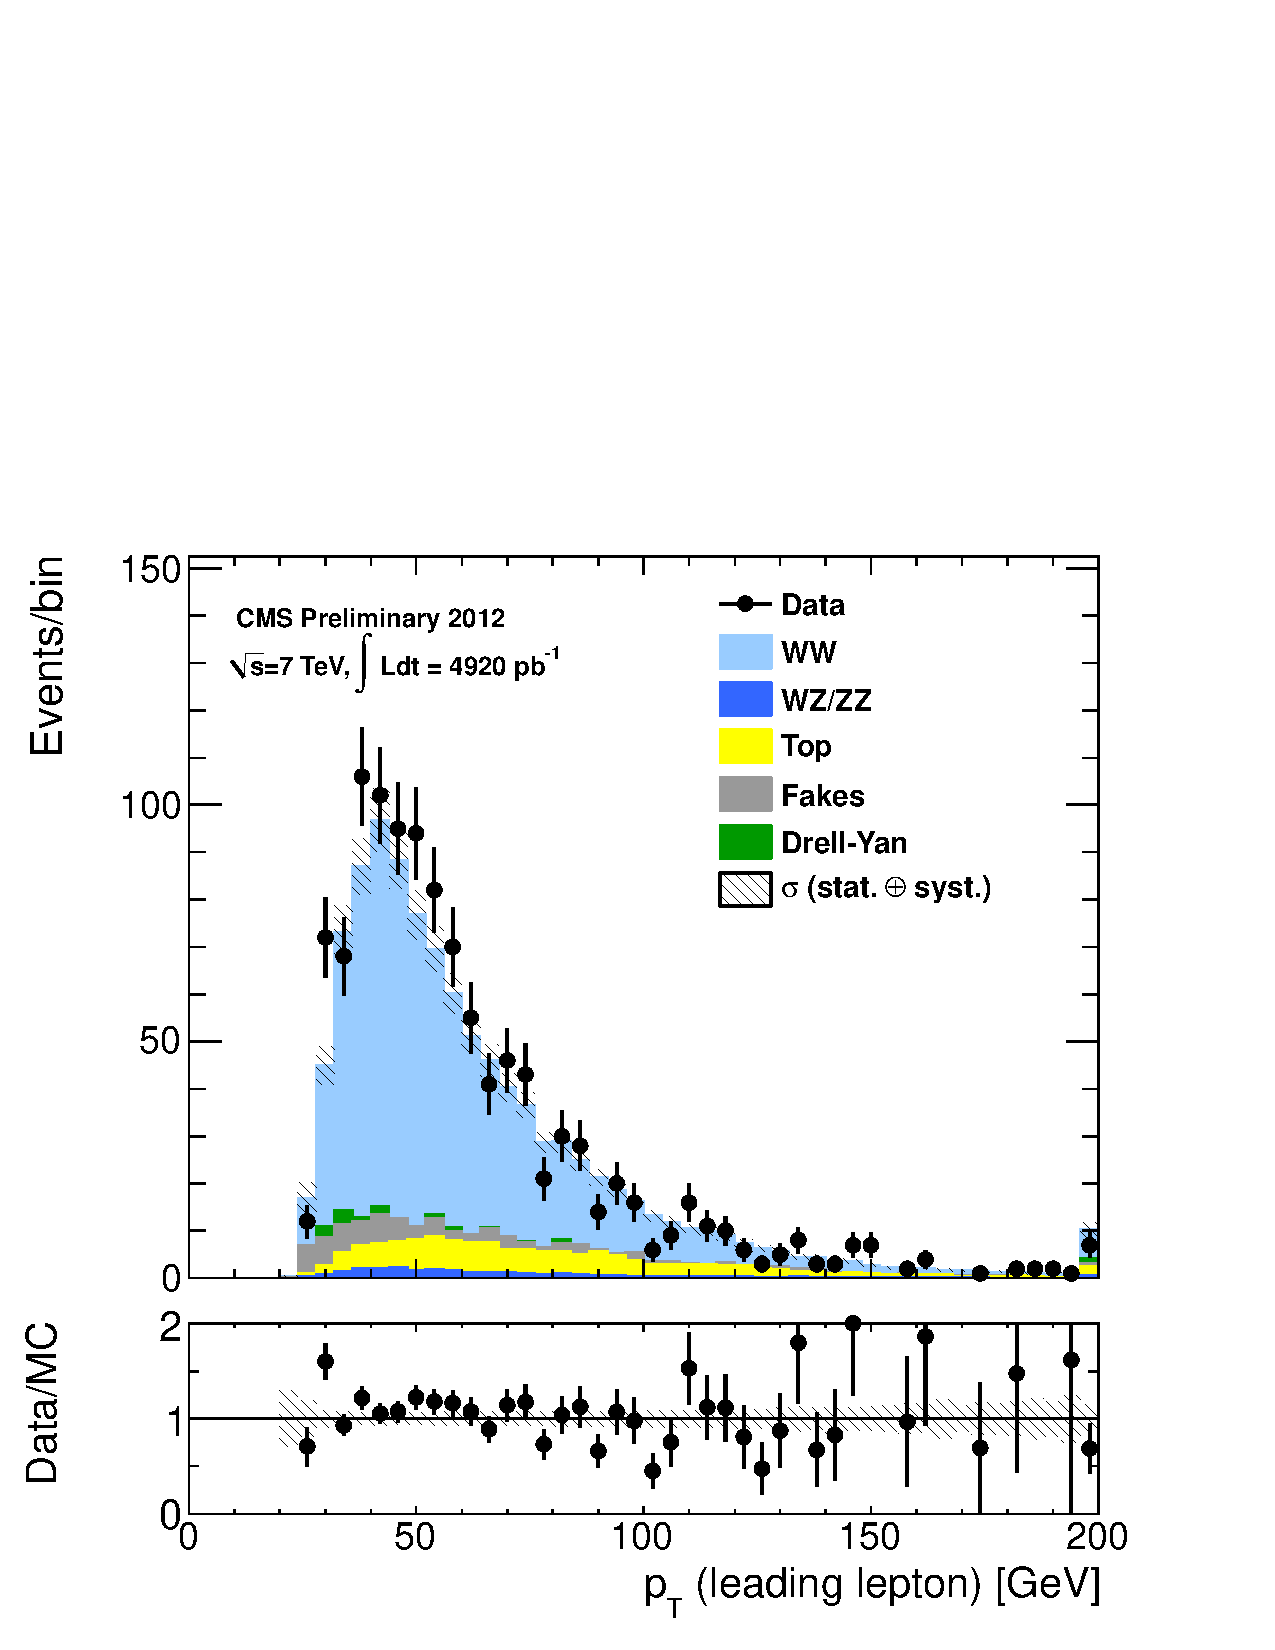
\includegraphics[width=.45\textwidth]{figures/pas_pt1_incl.pdf}}
\subfigure[Log scale]{\label{subfig:pas_pt1_incl_log}
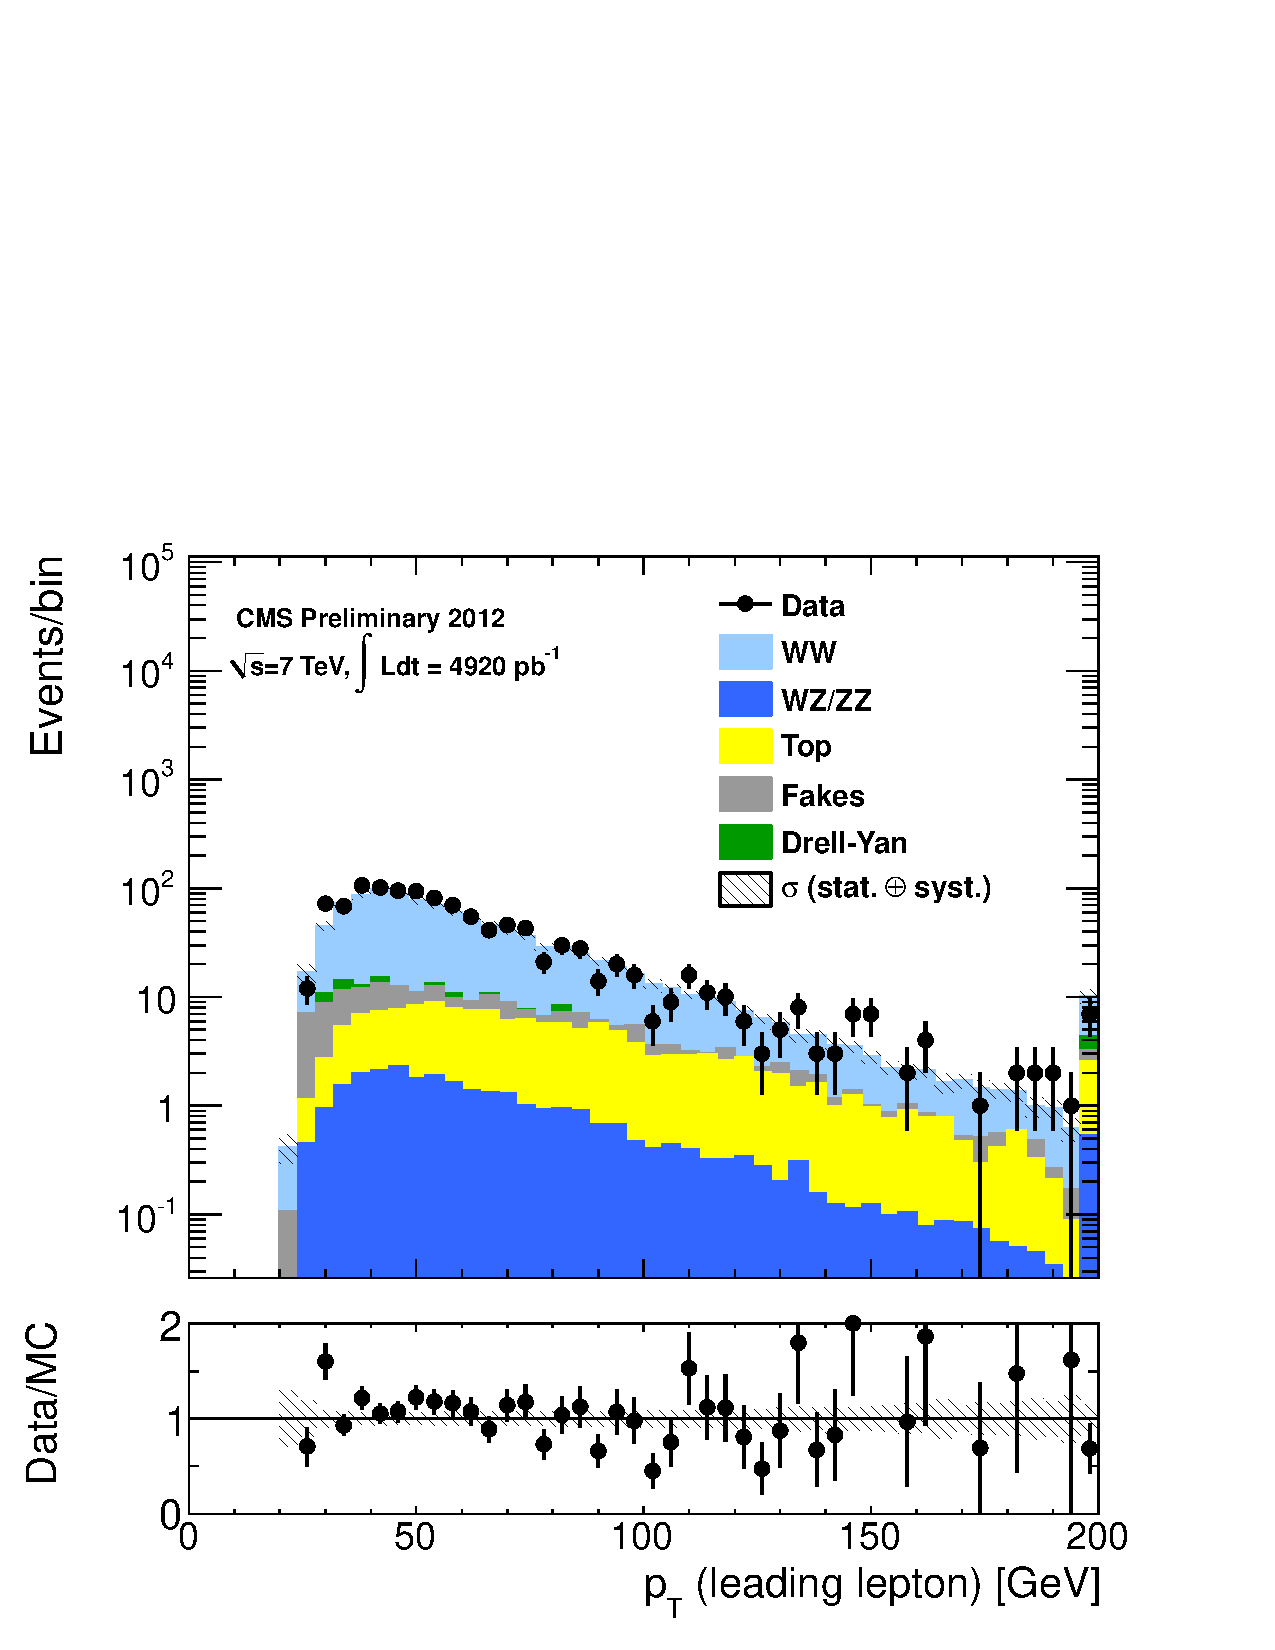
\includegraphics[width=.45\textwidth]{figures/pas_pt1_incl_log.pdf}}
\caption{Leading lepton \pt.}
\label{fig:pas_pt1_incl}
\end{figure}


\section{Data Samples}
  \label{sec:datasets}
  %UPDATEME%
The datasets used for this analysis are summarized in Tables.~\ref{tab:DatasetsData} 
and~\ref{tab:DatasetsMC} for data and Monte Carlo, respectively. The total integrated
luminosity is 49 $\pm$ 2 $\ipb$. We used just basic quality requirements, since an official good 
run list (JSON file) was not available. It will be used in future updates.
For Monte Carlo simulation we use madgraph when possible, 
but different generators such as Pythia and Powheg 
are also used. 
%For $gg \to \WW$ a dedicated generator is used. For \wz\ and \zz\
%processes we use Pythia, since MadGraph samples are mixed with $\WW$ in
%a single $VV$ sample, which is difficult to use properly.

%The choice of the Monte Carlo samples depends on the sample
%availability, but in general we tried to be consistent and use a
%single generator - MadGraph. In the case of Drell-Yan, MadGraph samples
%are not adequate to cover the full mass spectrum. The main sample has a 50 $\GeVcc$ 
%minimum dilepton mass requirement, while the other one, covering
%the low mass region, has an additional requirement on extra jet
%activity. 
%We use madgraph when possible, but different generators are used for some samples
%For $gg \to \WW$ a dedicated generator is used. For \wz\ and \zz\
%processes we use Pythia, since MadGraph samples are mixed with $\WW$ in
%a single $VV$ sample, which is difficult to use properly.

%UPDATEME%
\begin{table}[!ht]
\begin{center}
\begin{tabular}{|c|c|}
\hline
 Dataset Description                   &   Dataset Name   \\
\hline
\hline
\multicolumn{2}{|c|}{$H \to \WW$ Signal Selection Samples} \\
\hline
Run2011A MuEl PromptReco            &  /MuEG/Run2011A-PromptReco-v*/AOD   \\
Run2011A DiMuon PromptReco          &  /DoubleMu/Run2011A-PromptReco-v*/AOD   \\
Run2011A SingleMuon PromptReco      &  /SingleMu/Run2011A-PromptReco-v*/AOD   \\
Run2011A DiElectron PromptReco      &  /DoubleElectron/Run2011A-PromptReco-v*/AOD   \\
\hline
\hline
\multicolumn{2}{|c|}{Fake Rate Measurement Samples} \\
\hline
Run2010A Jet  PromptReco            & /Jet/Run2011A-PromptReco-v*/AOD	\\
Run2010B Photon PromptReco          & /Photon/Run2011A-PromptReco-v*/AOD \\
\hline
\end{tabular}
\caption{Summary of data datasets used.\label{tab:DatasetsData}}
\end{center}
\end{table}

\begin{table}[!ht]
\begin{center}
{\footnotesize
\begin{tabular}{|c|c|c|}
\hline
\multicolumn{3}{|c|}{With Pileup: Processed dataset name is always} \\
\multicolumn{3}{|c|}{/Spring11-PU\_S1\_START311\_V1G1-v*/AODSIM} \\
\hline
 Dataset Description                     &   Primary Dataset Name   & cross-section (pb)\\
\hline
qq $\rightarrow WW$                  	 &   /VVJetsTo4L\_TuneD6T\_7TeV-madgraph-tauola                        &  43.0  \\
gg $\rightarrow WW \to 2l 2\nu$          &   /GluGluToWWTo4L\_TuneZ2\_7TeV-gg2ww-pythia6                       &   0.153\\
$\ttbar$                              	 &   /TTJets\_TuneZ2\_7TeV-madgraph-tauola                             & 157.5 \\
$\singletops$                  	 	 &   /TToBLNu\_TuneZ2\_s-channel\_7TeV-madgraph                        &  1.4 \\
$\singletopt$                  	 	 &   /TToBLNu\_TuneZ2\_t-channel\_7TeV-madgraph                        &  20.9 \\
tW                                    	 &   /TToBLNu\_TuneZ2\_tW-channel\_7TeV-madgraph                       &  10.6 \\
Z[20-inf] $\rightarrow ee$	  	 &   /DYToEE\_M-20\_CT10\_TuneZ2\_7TeV-powheg-pythia                   &  1666.0 \\
Z[20-inf] $\rightarrow \mu\mu$        	 &   /DYToMuMu\_M-20\_CT10\_TuneZ2\_7TeV-powheg-pythia                 &  1666.0 \\	       
Z[20-inf] $\rightarrow \tau\tau$  	 &   /DYToTauTau\_M-20\_CT10\_TuneZ2\_7TeV-powheg-pythia-tauola        &  1666.0 \\
Z[10-20]  $\rightarrow ee$	  	 &   /DYToEE\_M-10To20\_CT10\_TuneZ2\_7TeV-powheg-pythia               &  3892.9 \\
Z[10-20]  $\rightarrow \mu\mu$    	 &   /DYToMuMu\_M-10To20\_CT10\_TuneZ2\_7TeV-powheg-pythia             &  3892.9 \\
Z[10-20]  $\rightarrow \tau\tau$  	 &   /DYToTauTau\_M-10To20\_CT10\_TuneZ2\_7TeV-powheg-pythia-tauola    &  3892.9 \\
W/Z+$\gamma$                       	 &   /PhotonVJets\_7TeV-madgraph                                       &  165.0 \\
W $\rightarrow$ $\ell\nu$           	 &   /WJetsToLNu\_TuneZ2\_7TeV-madgraph-tauola                         &  31314.0 \\
WZ                               	 &   /WZtoAnything\_TuneZ2\_7TeV-pythia6-tauola                        &  18.2 \\
ZZ                               	 &   /ZZtoAnything\_TuneZ2\_7TeV-pythia6-tauola                        &   5.9\\
$gg \to H \to WW \to 2\ell2\nu$          &   /GluGluToHToWWTo2L2Nu\_M-*\_7TeV-powheg-pythia6                   & vary \\
$gg \to H \to WW \to \ell\tau2\nu$       &   /GluGluToHToWWTo2L2Nu\_M-*\_7TeV-powheg-pythia6                   & vary \\
$gg \to H \to WW \to 2\tau2\nu$          &   /GluGluToHToWWTo2Tau2Nu\_M-*\_7TeV-powheg-pythia6                 & vary \\
$qqH,~H \to WW \to 2\ell2\nu$            &   /VBF\_HToWWTo2L2Nu\_M-*\_7TeV-powheg-pythia6                      & vary \\
$qqH,~ H \to WW \to \ell\tau2\nu$	 &   /VBF\_HToWWTo2Tau2Nu\_M-*\_7TeV-powheg-pythia6                    & vary \\
$qqH,~H \to WW \to 2\tau2\nu$	         &   /VBF\_HToWWToLNuTauNu\_M-*\_7TeV-powheg-pythia6                   & vary \\
$WH/ZH/\ttbar H,~H\to WW$                &   /WH\_ZH\_TTH\_HToWW\_M-*\_7TeV-pythia6                            & vary \\
\hline
\hline
\end{tabular}
}
\caption{Summary of Monte Carlo datasets used.\label{tab:DatasetsMC}. The cross sections for a SM Higgs boson
is taken from the LHC Higgs cross-section working group~\cite{LHCHiggsCrossSectionWorkingGroup:2011ti}}
\end{center}
\end{table}

Due to details in the implementation of the Powheg calculation, the
resulting Higgs $\pt$ spectrum for $gg \to H$ has a much harder
spectrum compared with the most precise spectrum calculated to NNLO
with resummation to NNLL order, as illustrated in
Figure~\ref{fig:h160ww_pthiggs}(a). Therefore, the proper procedure is
to apply an event-by-event rewighting to the Powheg simulated
events. For the time being we correct the $gg \to H \to \WW$ jet bin
efficiency computed from the Powheg Monte Carlo sample, by a scale
factor which is approximately identical for all Higgs masses. The
scale factors applied to each jet bin in the Powheg simulation are
shown in Figure~\ref{fig:h160ww_pthiggs}(b). The jet definition is 
consitent with the one used in the analysis.

\begin{figure}[!htbp]
\begin{center}
   \subfigure[]{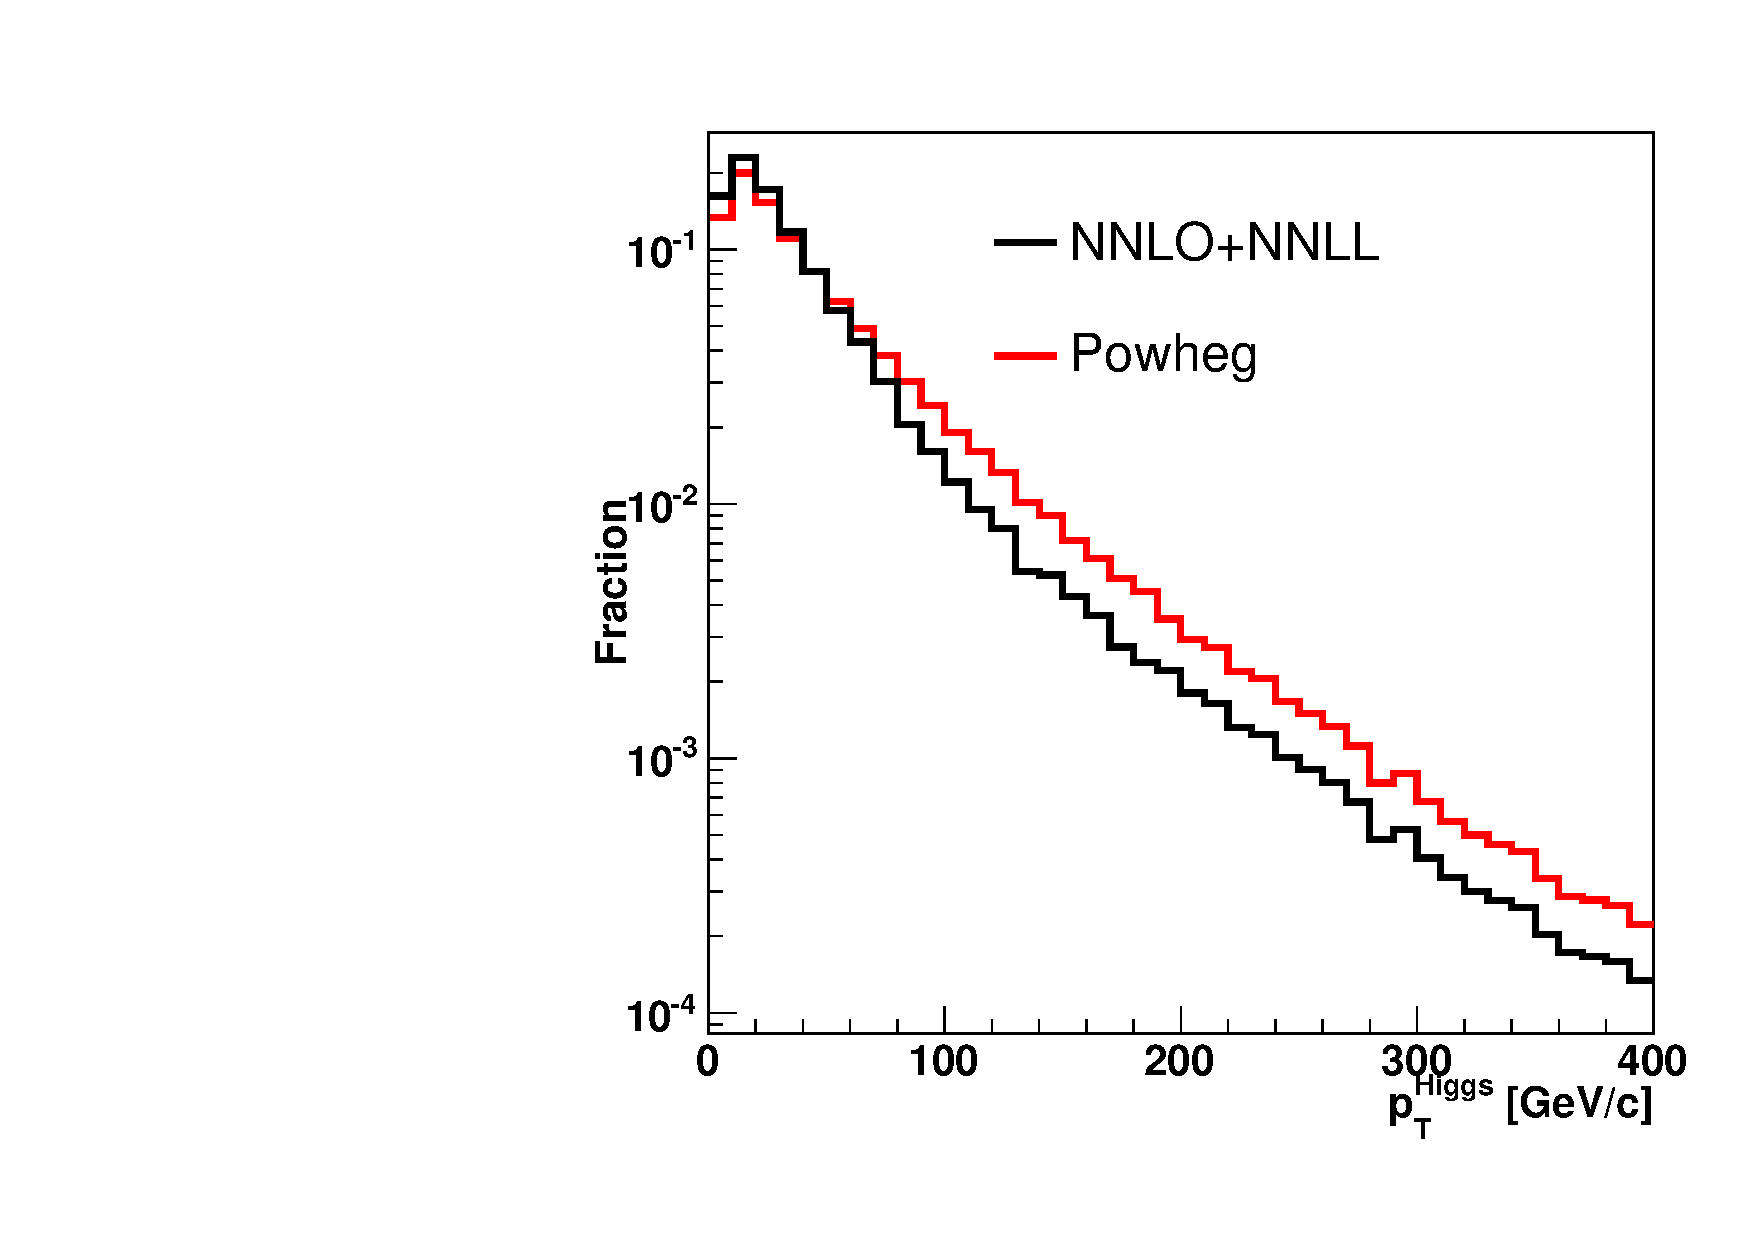
\includegraphics[width=0.49\textwidth]{figures/h160ww_pthiggs.pdf}}
   \subfigure[]{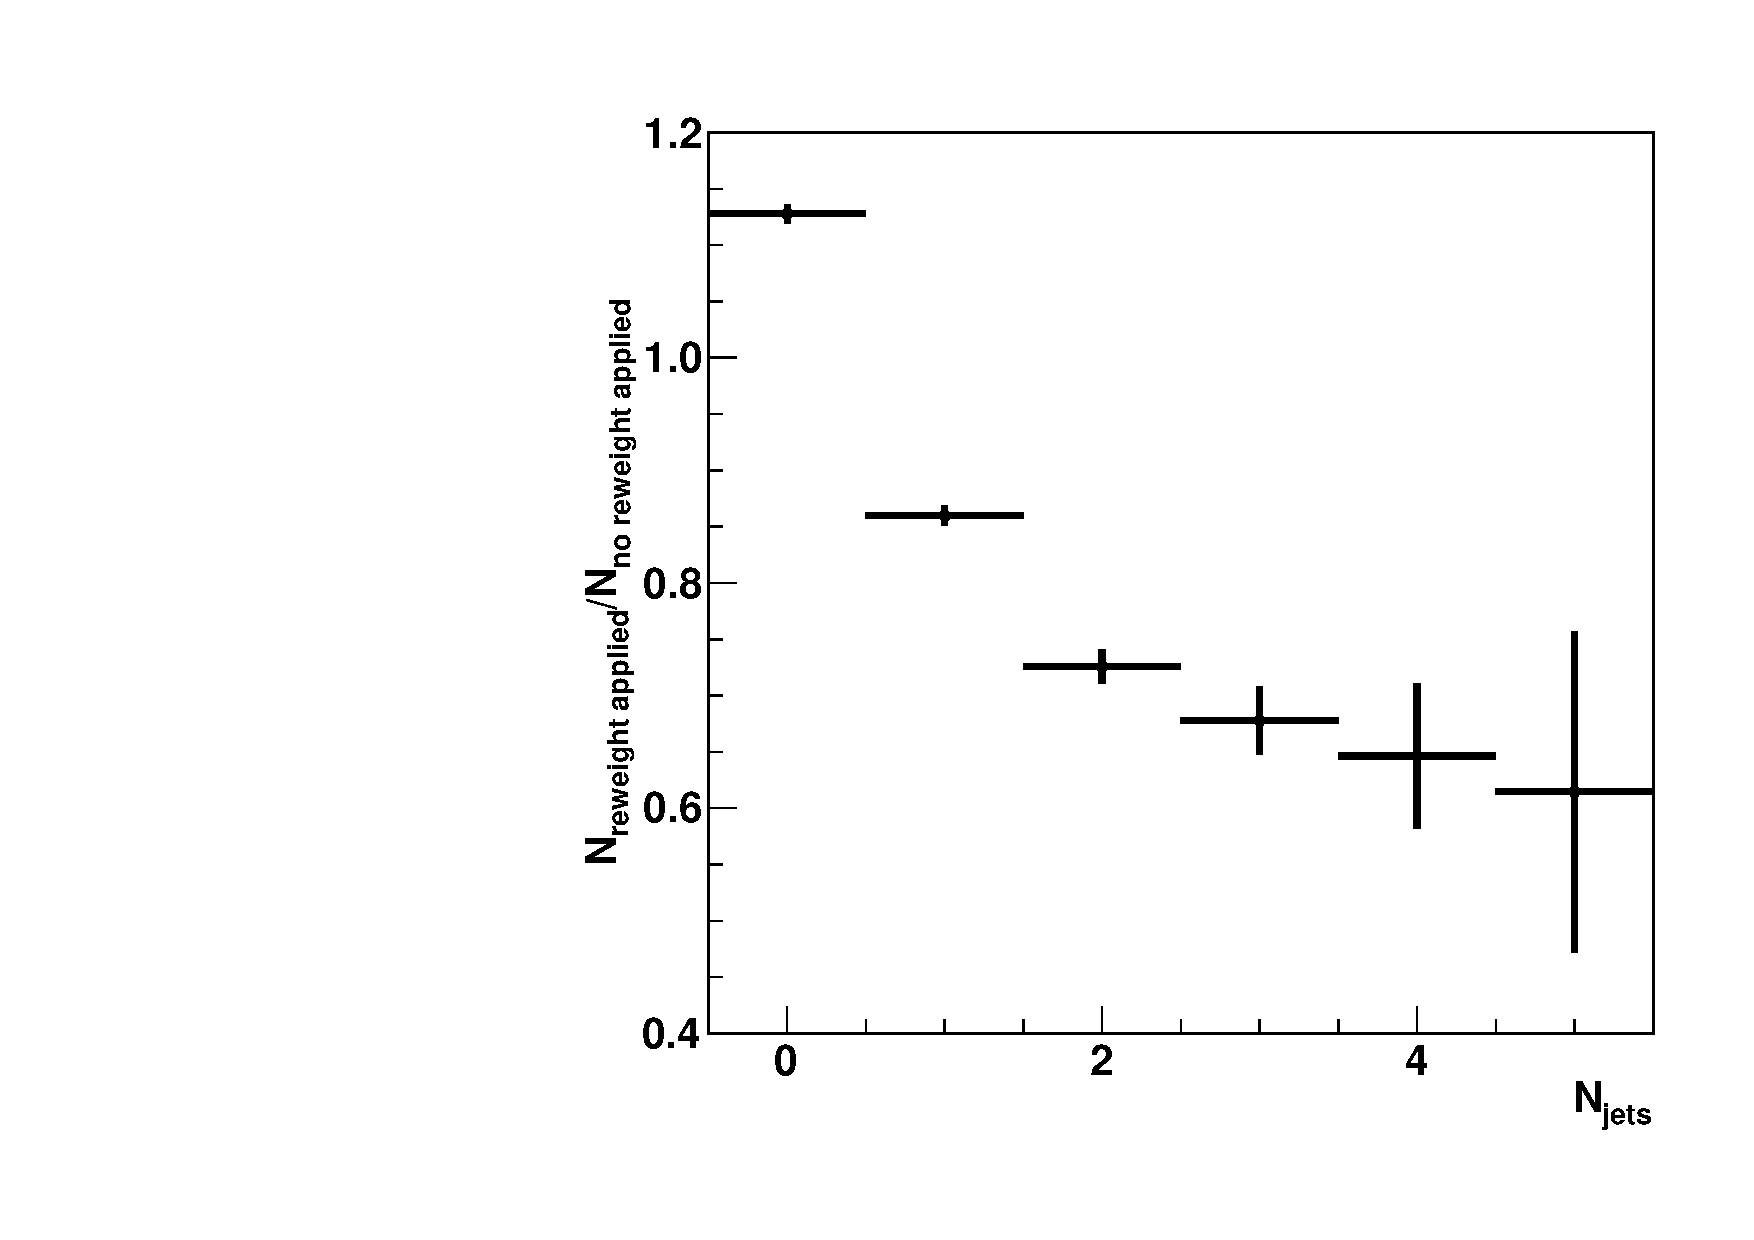
\includegraphics[width=0.49\textwidth]{figures/h160ww_njets_kfactor_ratio.pdf}} 
\caption{(a) Higgs transverse momentum spectrum as predicted by Powheg and the NNLO+NNLL calculation; (b) 
scale factors applied to each jet bin in the Powheg simulation.}
\label{fig:h160ww_pthiggs}
\end{center}
\end{figure}

\section{Event Selection}
  \label{sec:selection}
  The fully leptonic final state consists of two isolated leptons
and large missing energy from the two undetectable neutrinos.
The major reducible background processes are \ttbar{}, \wjets{} and Drell-Yan. 
We thus perform several steps to select and extract the $\WW$ signal from data:

\begin{enumerate}
    \item We select events that pass pre-defined lepton triggers.
    \item We then select those events with two oppositely charged 
    high $\pt$ isolated leptons ($ee$, $\mu\mu$, $e\mu$) requiring:
        \begin{itemize}    
            \item $\pt>20~\GeVc$ for both leptons;
            \item standard identification and isolation requirements 
	    on both leptons.
        \end{itemize}
     \item We reject events with more than zero reconstructed jets;
     \item large transverse missing energy due to the neutrinos.
\end{enumerate}

The selection steps are now described in detail in Ref. \cite{ref:WWXS2011}.


\section{Method}
   \label{sec:method}
   In order to fit for anomalous couplings we used a maximum likelihood fit in
the RooFit framework. Differences between the Standard Model
and anomalous couplings are established in the leading lepton
\pt\ distribution and the overall \ww\ event yield. The combined PDF for the
leading lepton \pt\ distribution is:
\begin{equation}
  P(\pt) = \frac{N^\mathrm{exp}_\mathrm{sig}}{N^\mathrm{exp}}P_\mathrm{sig}(\pt) + 
  \frac{N^\mathrm{exp}_\mathrm{bkg}}{N^\mathrm{exp}}P_\mathrm{bkg}(\pt) 
\end{equation}
where $P_\mathrm{sig}$ and $P_\mathrm{bkg}$ are signal and background PDFs of the
leading lepton \pt{}, $N^\mathrm{exp}_\mathrm{sig}$ and $N^\mathrm{exp}_\mathrm{bkg}$ are the expected
number of signal and background events and
$N^\mathrm{exp}=N^\mathrm{exp}_\mathrm{sig}+N^\mathrm{exp}_\mathrm{bkg}$.

The Likelihood is defined as a product of Poisson PDFs for the observed
number of events and the combined PDF for each event:
\begin{equation}
  L = e^{-N^\mathrm{exp}}(N^\mathrm{exp})^{N^\mathrm{obs}}\displaystyle\prod_{i=1}^{N^\mathrm{obs}}P(\pt)
\end{equation}

To account for statistical and systematic uncertainties in the
luminosity, cross-section and background estimation we assume
Gaussian distributions for the uncertainties and add corresponding
constraints to the Likelihood.

The signal PDF allows for parameterization of the leading lepton \pt\
PDF and the cross-section as functions of the anomalous
couplings. Since the effective Lagrangian is linear in the couplings
we can parametrize the leading lepton differential cross-section with
a 2D or 3D parabola ~\cite{ref:atgc_method}. In the fit the expected
number of signal events is taken from that parameterization. The
expected background yield is taken from the background estimation of
the \ww\ analysis~\cite{ref:wwnote}. Table~\ref{tab:xsections} shows
the reference points and the corresponding cross-sections used in the
model.

\begin{table}[!ht]
  \begin{center}
  \begin{tabular} {|c c c|c c|c|}
\hline
  $\lambda_Z$ & $\Delta g^Z_1$ & $\Delta\kappa_{\gamma}$ & $\Delta\kappa_Z$ & $\lambda_{\gamma}$ & $\sigma$ \\
  \hline
  0           & 0              & 0                       & 0                & 0                  & $547.541\pm1.947$~fb \\
  0           & 0              & $+0.7$                  & $-0.2205$        & 0                  & $617.147\pm1.604$~fb \\
  0           & 0              & $-0.7$                  & $+0.2205$        & 0                  & $633.939\pm1.671$~fb \\
  $+0.5$      & 0              & 0                       & 0                & $+0.5$             & $1223.832\pm3.414$~fb \\
  $-0.5$      & 0              & 0                       & 0                & $-0.5$             & $1193.115\pm3.026$~fb \\
  $+0.2$      & 0              & 0                       & 0                & $+0.2$             & $661.276\pm1.837$~fb \\
  $-0.2$      & 0              & 0                       & 0                & $-0.2$             & $648.021\pm1.630$~fb \\
  $+0.5$      & 0              & $+0.7$                  & $-0.2205$        & $+0.5$             & $1295.486\pm3.224$~fb \\
  $-0.5$      & 0              & $+0.7$                  & $-0.2205$        & $-0.5$             & $1267.807\pm2.971$~fb \\
  $-0.5$      & 0              & $-0.7$                  & $+0.2205$        & $-0.5$             & $1279.312\pm2.999$~fb \\
  $+0.5$      & 0              & $-0.7$                  & $+0.2205$        & $+0.5$             & $1319.705\pm2.920$~fb \\
  0           & $+0.75$        & 0                       & $+0.75$          & 0                  & $1284.979\pm2.875$~fb \\
  0           & $-0.75$        & 0                       & $-0.75$          & 0                  & $1370.808\pm2.905$~fb \\
  $+0.5$      & $-0.75$        & 0                       & $-0.75$          & $+0.5$             & $1766.015\pm4.324$~fb \\
  $-0.5$      & $-0.75$        & 0                       & $-0.75$          & $-0.5$             & $2295.906\pm4.985$~fb \\
  $-0.5$      & $+0.75$        & 0                       & $+0.75$          & $-0.5$             & $1644.440\pm4.276$~fb \\
  $+0.5$      & $+0.75$        & 0                       & $+0.75$          & $+0.5$             & $2245.131\pm5.315$~fb \\

 \hline
  \end{tabular}

  \caption{Exclusive cross-section for $\WW\to\mu\mu$ with anomalous
  couplings. Inclusive Standard Model \WW\ cross-section is
  $0.548/(0.108)^2=47.0$pb.}

   \label{tab:xsections}
  \end{center}
\end{table}


Figure~\ref{fig:pdfs} shows the result of the signal PDF
parameterization using non-parametric PDFs based on histograms. It
reveals reasonable agreement between the initial PDFs from the
generated samples and the final aTGC model.

\begin{figure}[tp]
  \centerline{
    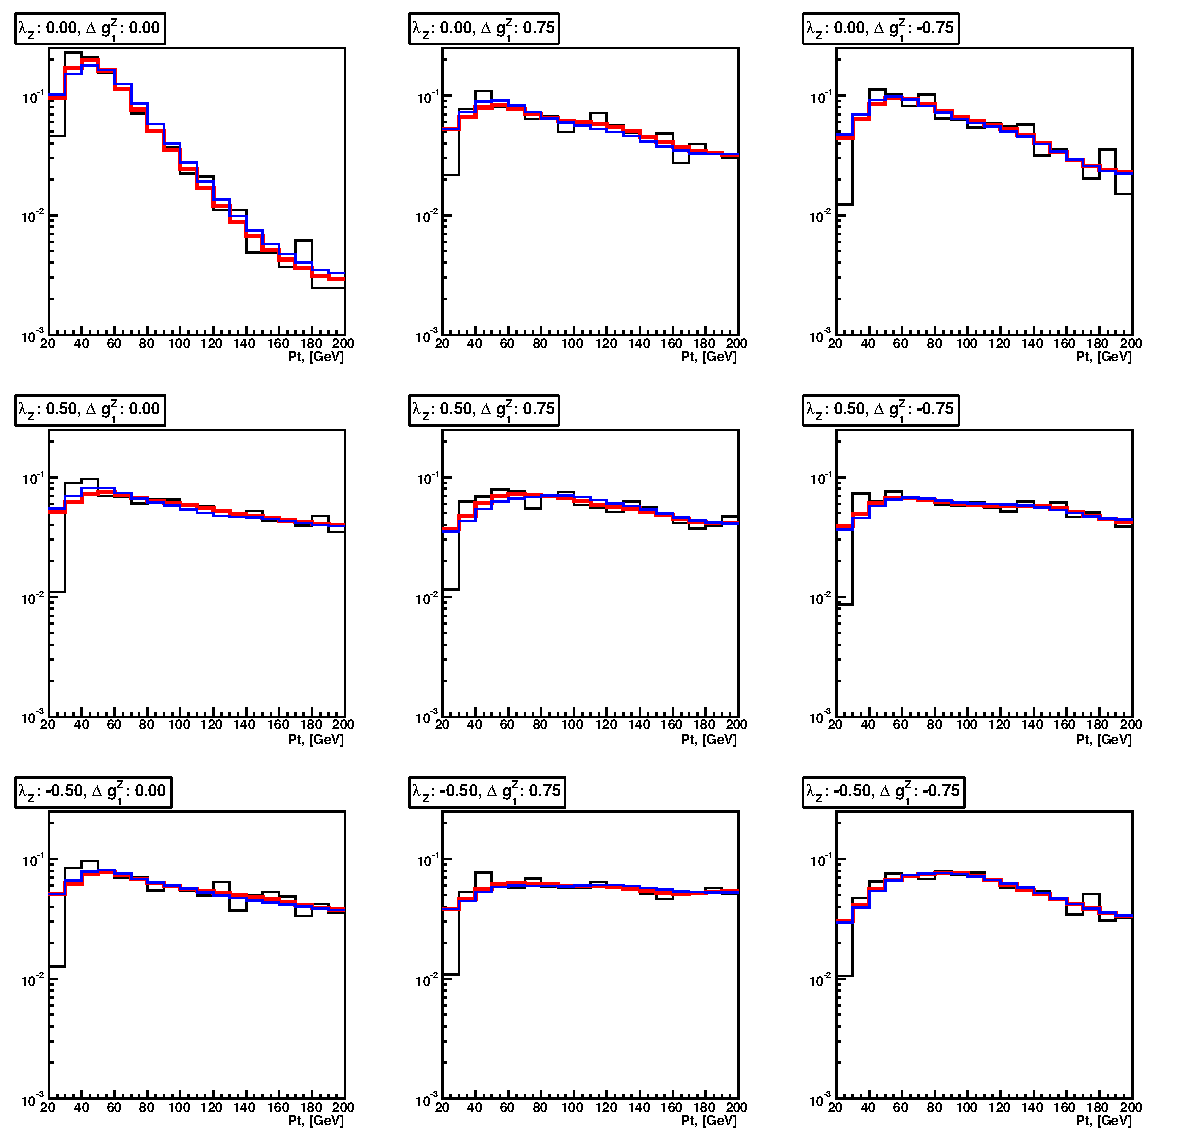
\includegraphics[width=1.0\textwidth]{figures/pdfs}
  }

  \caption[PDF parameterization] {Leading lepton \pt\ distributions
  for \ww\ events with and without aTGCs. The black points represent the
  true \pt\ distribution for Monte Carlo events that passed the final
  selection. The blue dots show the \pt\ distribution from the model used to
  parametrize the anomalous coupling effects across different values
  of the couplings.}
\label{fig:pdfs}
\end{figure}

Figure~\ref{fig:bkgpdfs} shows the leading lepton \pt\ PDFs
for background events. It is important to note that some of the major
backgrounds have harder leading lepton \pt\ distributions than Standard
Model $WW$, which may bias the result if not handled properly.

\begin{figure}[tp]
  \centerline{
    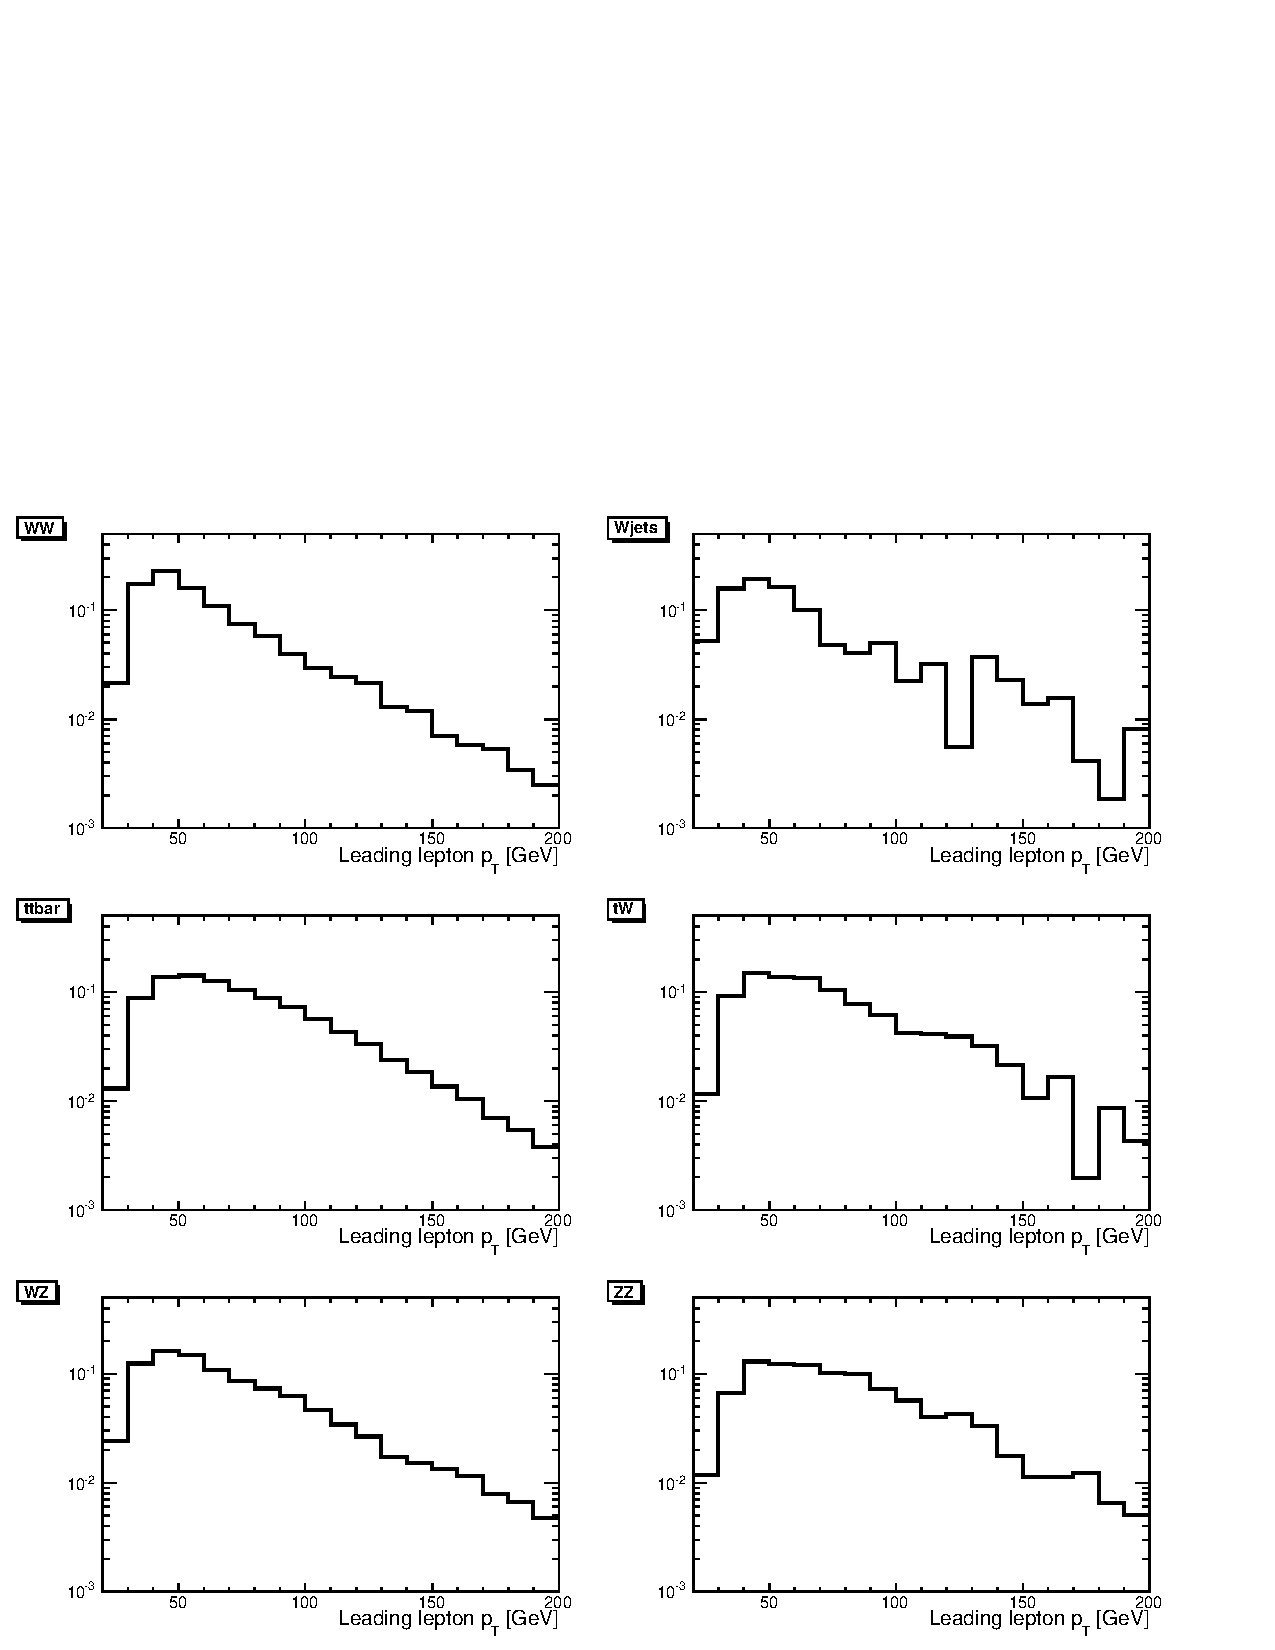
\includegraphics[width=0.7\textwidth]{figures/pdf_mc_all.pdf}
  }

  \caption[Background PDFs] {Leading lepton \pt\ PDFs for background
  events after full event selection.} \label{fig:bkgpdfs}
\end{figure}

\section{Existing limits}
   \label{sec:limits}
   % \fixme{Make sure it's all up to date}
The current best fit results for anomalous couplings are dominated by LEP
results. Table~\ref{tab:limits} shows the existing limits for various
couplings~\cite{ref:atgc_d0,ref:pdg}

\begin{table}[htp]
\caption[Current limits on anomalous couplings] {Current limits on
  anomalous couplings. The world best limits are based on a fit of LEP
  measurements. Tevatron results are shown for comparison. }
\begin{center}
\begin{tabular}{|c|c|}
\hline
 Coupling & Particle Data Group Fit \\
\hline
$\Lambda_\gamma$      & $-0.028^{+0.020}_{-0.021}$ \\
$\Lambda_Z$           & $-0.088^{+0.060}_{-0.057}$ \\
$\Delta g^Z_1$        & $-0.016^{+0.022}_{-0.019}$ \\
$\Delta\kappa_\gamma$ & $-0.027^{+0.044}_{-0.045}$ \\
$\Delta\kappa_Z$      & $-0.026^{+0.059}_{-0.056}$ \\
\hline
\end{tabular}
\begin{tabular}{|c|c|c|}
\hline
 Coupling & Tevatron ($\ww+\wz\to\ell\nu2\mathrm{jet}$) & Tevatron (\wwlulu{}) \\
\hline
$\Lambda=\Lambda_\gamma=\Lambda_Z$      & [-0.10,0.11] at 95\% C.L. & [-0.14,0.18] at 95\% C.L. \\
$\Delta\kappa_\gamma$                   & [-0.44,0.55] at 95\% C.L. & [-0.54,0.83] at 95\% C.L. \\
$\Delta g^Z_1$                          & [-0.12,0.20] at 95\% C.L. & [-0.14,0.30] at 95\% C.L. \\
\hline
\end{tabular}
\end{center}
\label{tab:limits}
\end{table}

\section{Monte Carlo modeling of anomalous couplings}
   \label{sec:modeling}
   We use MCFM NLO generator to produce the leading lepton \pt\
distributions for a number of points with non-zero anomalous
couplings. The distributions are corrected for the acceptance and
lepton reconstruction efficiency derived from a fully simulated Monte
Carlo sample. The Standard Model distribution has very few events for
large values of the leading lepton pt. It is hard to get large enough
sample of events generated with MCFM to cover this region. Therefore
we rely on the nominal Madgraph WW Monte Carlo to get the leading
lepton \pt\ distribution for the case of zero anomalous couplings. A
comparison of the distributions from different generators can be seen
in Figure~\ref{fig:generator_comparison}. It shows a good agreement
between Madgraph and MCFM distribtions.

\begin{figure}[tp]
  \centerline{
    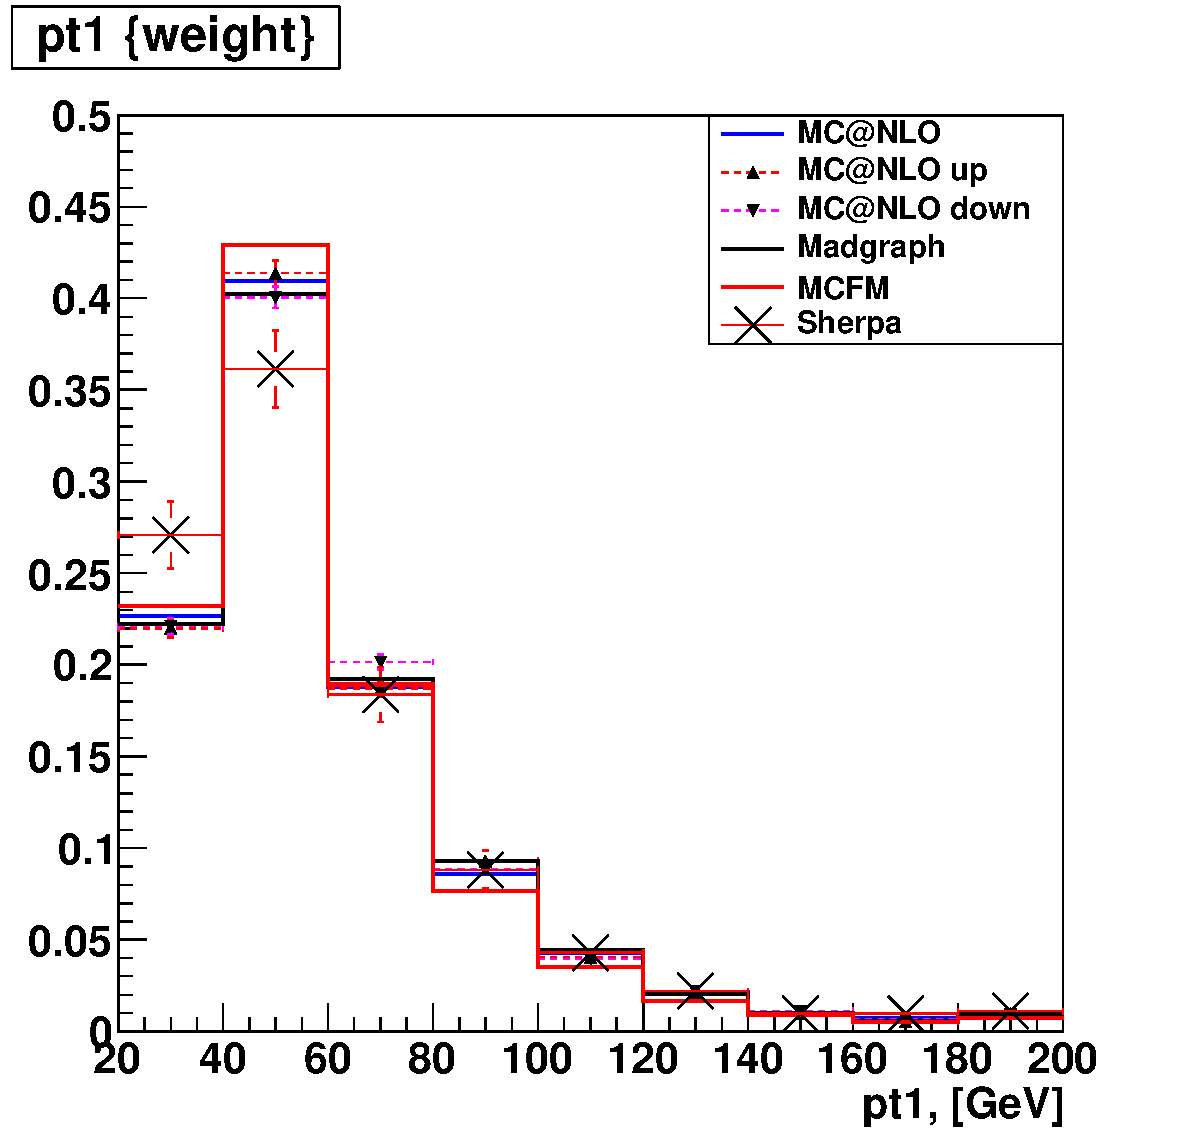
\includegraphics[width=0.6\textwidth]{figures/generator_comparison.pdf}
%    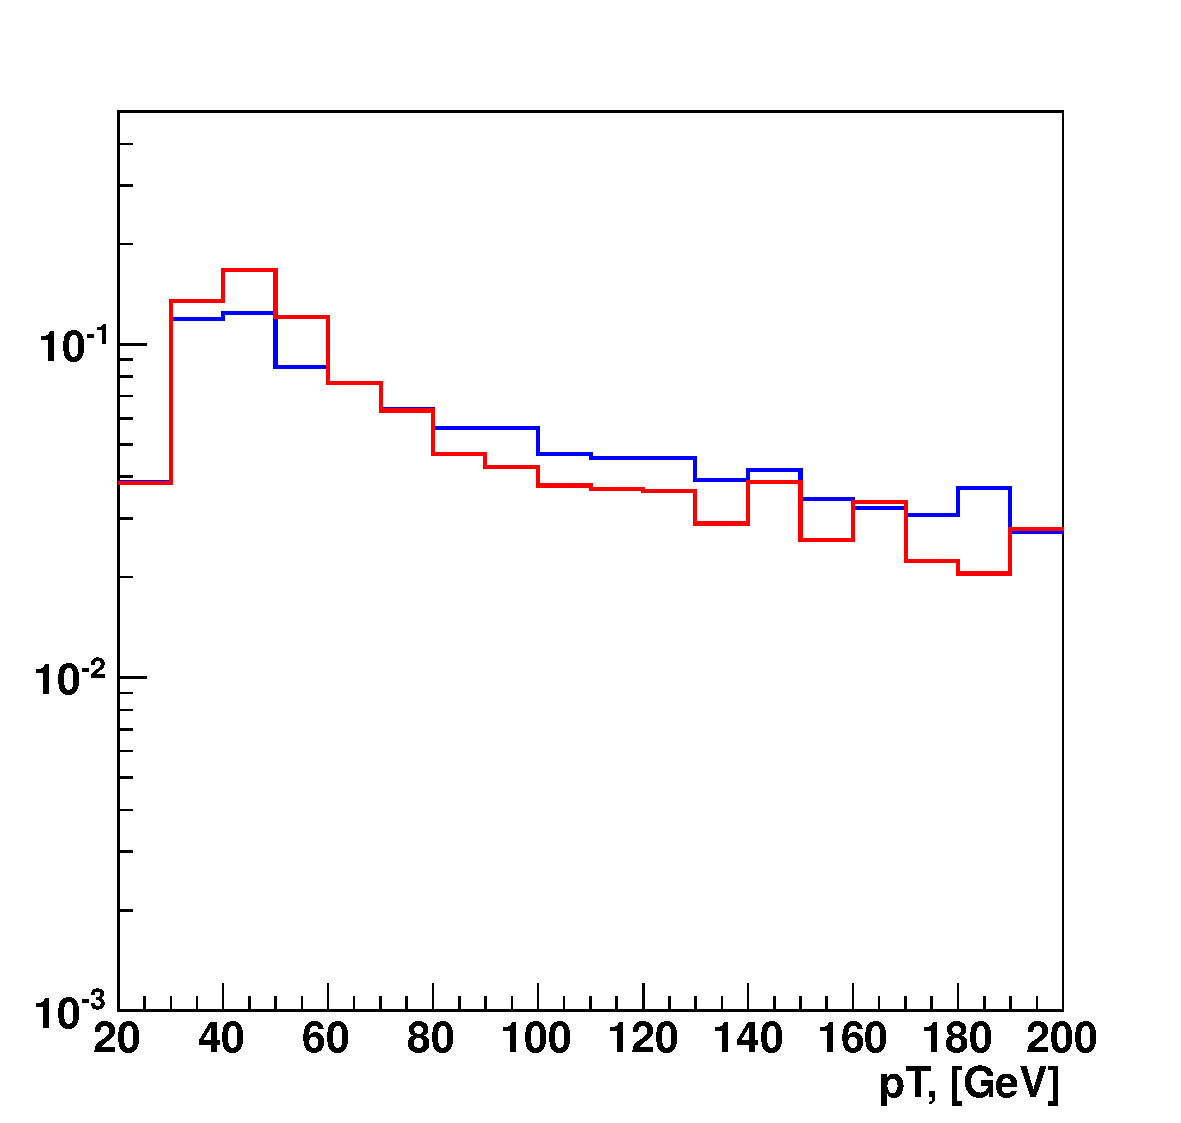
\includegraphics[width=0.45\textwidth]{figures/generator_comparison_atgc.pdf}
  }

  \caption[Generator comparison]{Leading lepton \pt\ distribution
  for \WW\ simulated data using Madgraph (full simulation), MC@NLO (full simulation),
  Sherpa (fast simulation) and MCFM (reweighted). No aTGC.}

  \label{fig:generator_comparison}
\end{figure}

It is important to confirm that all the distributions are consistent
with the model used to parametrize the leading lepton \pt\ for
arbitrary couplings. Figure~\ref{fig:pdfs} shows the result of the signal PDF
parameterization using non-parametric PDFs based on histograms. It
reveals good agreement between the initial PDFs from the
generated samples and the final aTGC model.

\begin{figure}[tp]
  \centerline{
    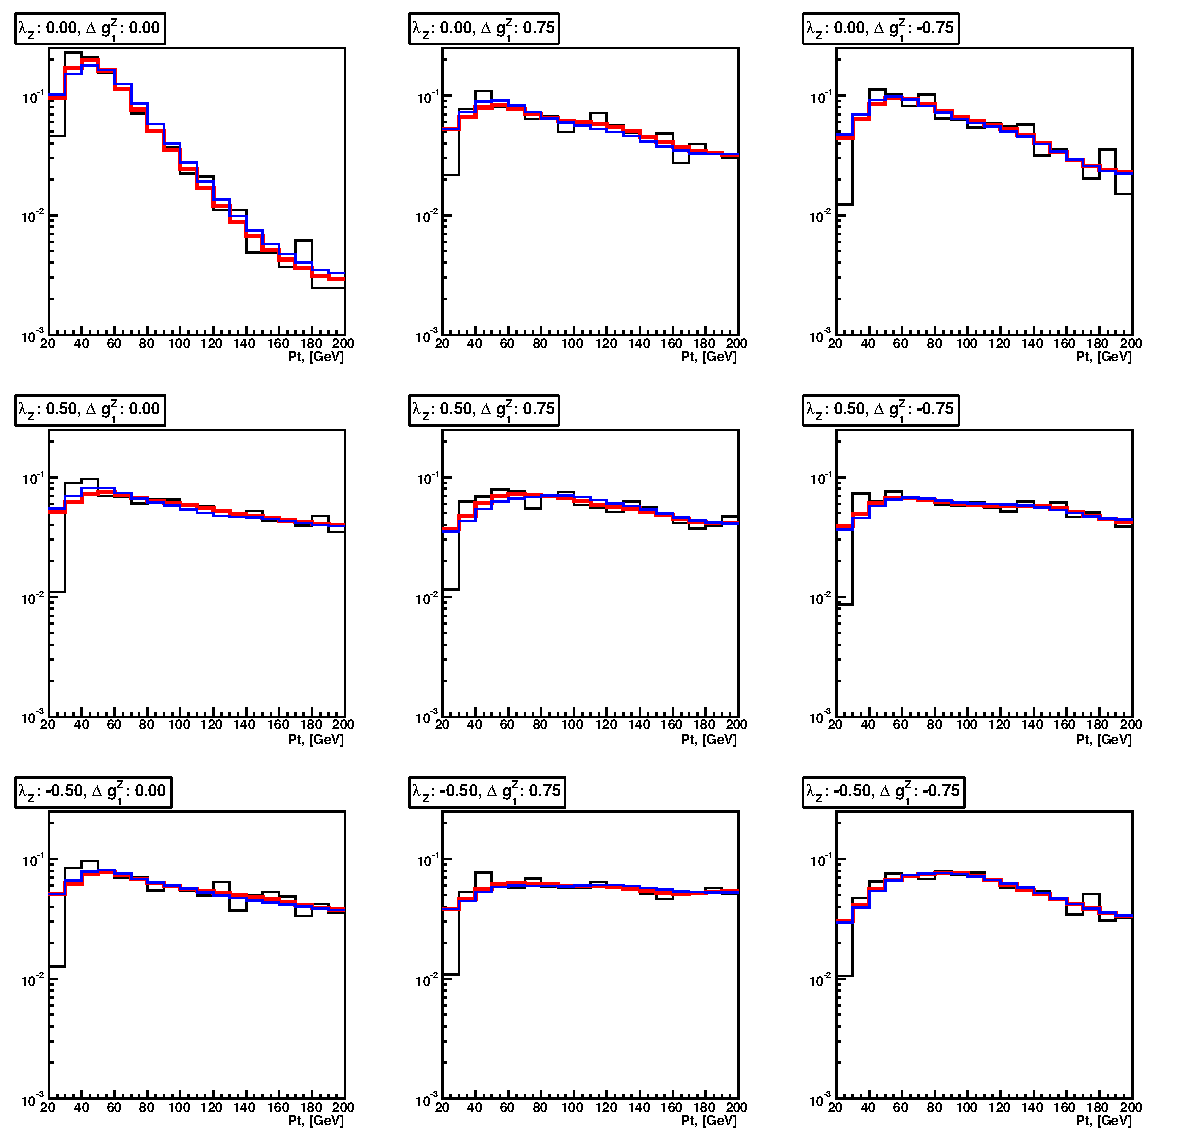
\includegraphics[width=1.0\textwidth]{figures/pdfs}
  }

  \caption[PDF parameterization] {Leading lepton \pt\ distributions
  for \ww\ events with and without aTGCs. The black points represent the
  true \pt\ distribution for Monte Carlo events that passed the final
  selection. The blue dots show the \pt\ distribution from the model used to
  parametrize the anomalous coupling effects across different values
  of the couplings.}
\label{fig:pdfs}
\end{figure}


\clearpage
\section{Standard Model \ww\ yields}
   \label{sec:smww}
   
Table~\ref{tab:bkg_estimation} summarizes the estimation of background
yields using primarily data driven methods as described in Ref. \cite{ref:WWXS2011}.

\begin{table}[!ht]
  \begin{center}
 {\small
  \begin{tabular} {|c|c|c|c|c|c|c|}
\hline
      &   data & all bkg. & $qq \to \WW$ & $gg \to \WW$ &  $\ttbar+tW$   & $\Wjets$    \\
\hline
\hline
% $ee+\mu\mu$    &  462 & 94.8 $\pm$  4.4 & 296.8 $\pm$  2.7 & 17.7 $\pm$  0.4 & 43.8 $\pm$  1.3 & 15.9 $\pm$  2.3 \\ 
% $e\mu + \mu e$ &  668 & 146.4 $\pm$  4.8 & 477.2 $\pm$  3.4 & 28.2 $\pm$  0.5 & 77.8 $\pm$  1.8 & 42.4 $\pm$  3.2 \\ 
% Total & 1130   & 241.1 $\pm$  6.5 & 774.0 $\pm$  4.4 & 45.9 $\pm$  0.6 & 121.6 $\pm$  2.2 & 58.3 $\pm$  3.9 \\ 
% add syst as well
 $ee+\mu\mu$ &  462 & 94.8 $\pm$ 12.7 & 296.8 $\pm$ 22.2 & 17.7 $\pm$  5.5 & 43.8 $\pm$  8.5 & 15.9 $\pm$  6.2 \\ 
  $e\mu + \mu e$ &  668 & 146.4 $\pm$ 22.2 & 477.2 $\pm$ 33.8 & 28.2 $\pm$  8.7 & 77.8 $\pm$ 15.0 & 42.4 $\pm$ 15.6 \\ 
  Total & 1130 & 241.1 $\pm$ 33.0 & 774.0 $\pm$ 55.8 & 45.9 $\pm$ 14.1 & 121.6 $\pm$ 23.4 & 58.3 $\pm$ 21.3 \\ 
 \hline
  \end{tabular}
  }

 {\small
  \begin{tabular} {|c|c|c|c|c|}
 \hline
   & $WZ$/$ZZ$ & $\dyll$ & $W+\gamma$ & \dytt \\
\hline
\hline

% $ee+\mu\mu$    & 18.1 $\pm$  0.4 & 11.7 $\pm$  3.2 &  5.3 $\pm$  1.4 &  0.0 $\pm$  0.0 \\ 
% $e\mu + \mu e$ & 11.0 $\pm$  0.2 &  0.0 $\pm$  0.0 & 14.5 $\pm$  3.1 &  0.8 $\pm$  0.2 \\ 
% Total          & 29.1 $\pm$  0.4 & 11.7 $\pm$  3.2 & 19.8 $\pm$  3.4 &  0.8 $\pm$  0.2 \\ 
% add syst as well
 $ee+\mu\mu$ & 18.1 $\pm$  1.3 & 11.7 $\pm$  6.8 &  5.3 $\pm$  1.9 &  0.0 $\pm$  0.0 \\ 
 $e\mu + \mu e$ & 11.0 $\pm$  1.1 &  0.0 $\pm$  0.0 & 14.5 $\pm$  4.6 &  0.8 $\pm$  0.2 \\ 
 Total & 29.1 $\pm$  2.2 & 11.7 $\pm$  6.8 & 19.8 $\pm$  5.7 &  0.8 $\pm$  0.2 \\ 
\hline
  \end{tabular}
  }
  \caption{Expected number of signal and background events for an
  integrated luminosity of \intlumi, together with the data event yields, after
  applying the full selection. Statistical and systematic uncertainties are
  included.}
   \label{tab:bkg_estimation}
  \end{center}
\end{table}


\section{Fit validation}
   \label{sec:validation}
   The validation of the maximum likelihood fit, used to extract all information in this
analysis, is now described. The validation procedure consists of
two main tests. The first test is a fit using a data sample without
anomalous couplings. Such a test allows to identify problems with
event generation causing discrepancies in the leading lepton
\pt\ distribution. The second test is a fit using a data sample with
anomalous couplings. Such a test checks if we can properly measure
anomalous couplings when they are present. Both tests are critical to
validate the fitting tools, which are fairly complicated.

In the previous analysis it was found that the leading lepton
\pt\ distribution does not allow to differentiate between different
couplings and a typical observation inconsistent with Standard Model
represents a class of possible coupling values.

Figure~\ref{fig:val_scans} shows fit results and likelihood scans for
\ww\ simulated data with and without anomalous couplings. One may
conclude that even though the fit was able to measure the couplings
close to the true values, there is large uncertainty on the angle
between the two couplings as is revealed in the shapes of the contour
plots in the likelihood scans.

\begin{figure}[tp]
  \centerline{
    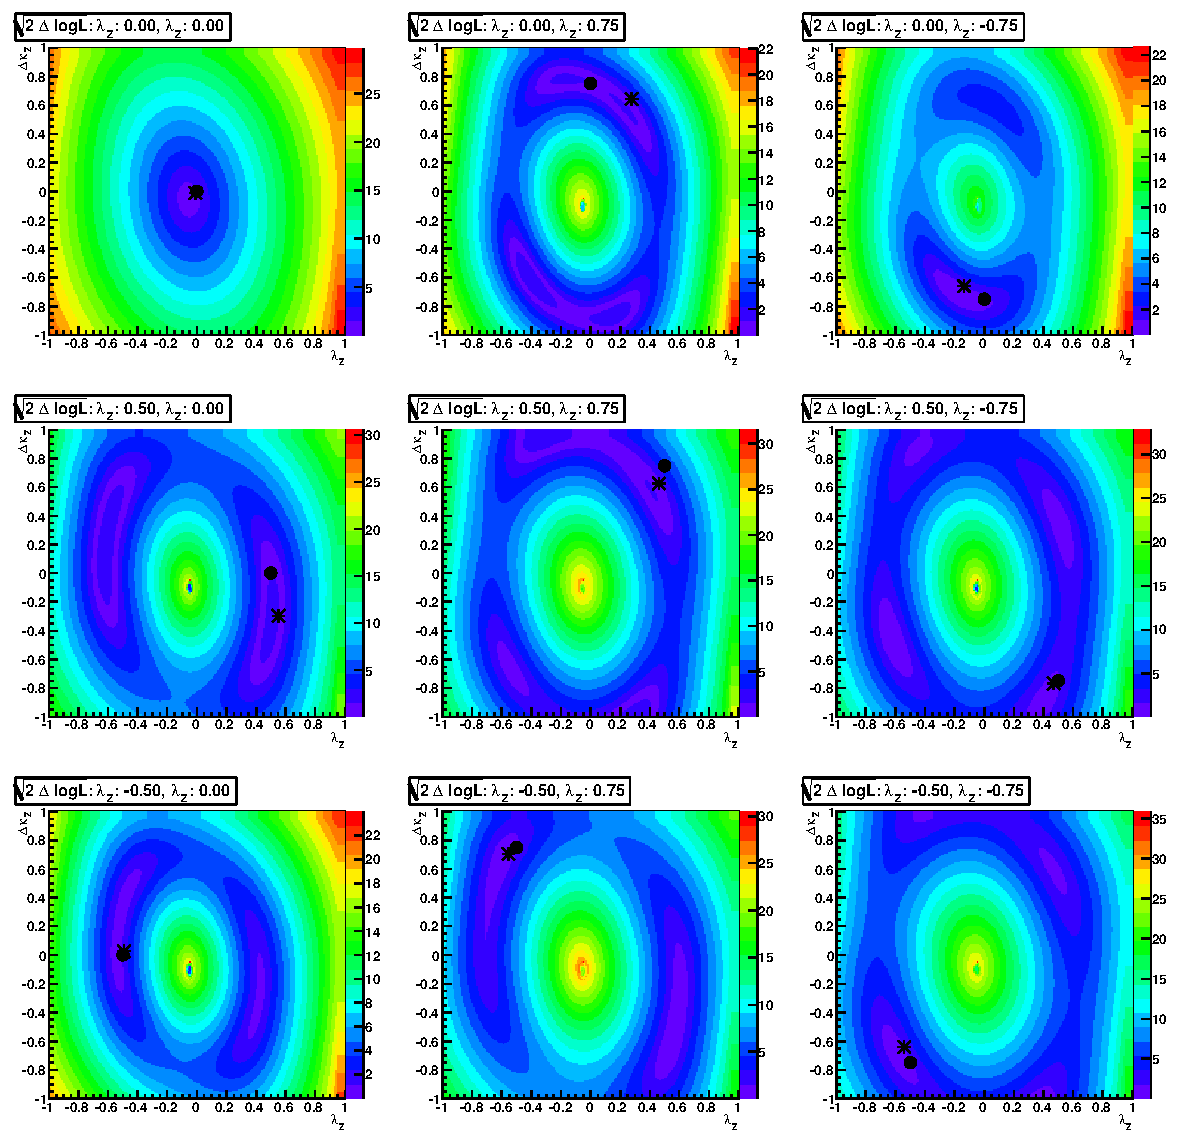
\includegraphics[width=1.0\textwidth]{figures/validation_likelihood_scans}
  }

  \caption[Likelihood scan for Signal Monte Carlo] {Likelihood scans
    for 350/pb of data excluding backgrounds. The curves
    represent the $\sqrt{2\Delta\log L}$ 1D significance of the difference between the
    likelihood with the sample's true anomalous couplings and the other
    values on the plain. The black star is the fit result when both couplings are
    allowed to float in the fit. The black point is the true value of the couplings.}
  \label{fig:val_scans}
\end{figure}

\subsection{Pseudo-experiments}
Figures~\ref{fig:fit_ww_mc_1D} and \ref{fig:fit_wwATGC_mc_1D_abs} show
results of the fits on \ww\ Monte Carlo samples with and without
anomalous couplings and excluding backgrounds. If only one coupling is
fitted it is not possible to get the sign right, so only absolute
values can be measured.

Pseudo-experiments with Standard Model \ww\ Monte Carlo are performed to look
for bias in the fit for the central value and to test the uncertainty
estimation. No significant deviation from zero is
found. Pseudo-experiments with non-zero anomalous couplings underestimate 
the true value by 20-30\%. To take this effect into
account we rescale final results.

\begin{figure}[tp]
  \centering
    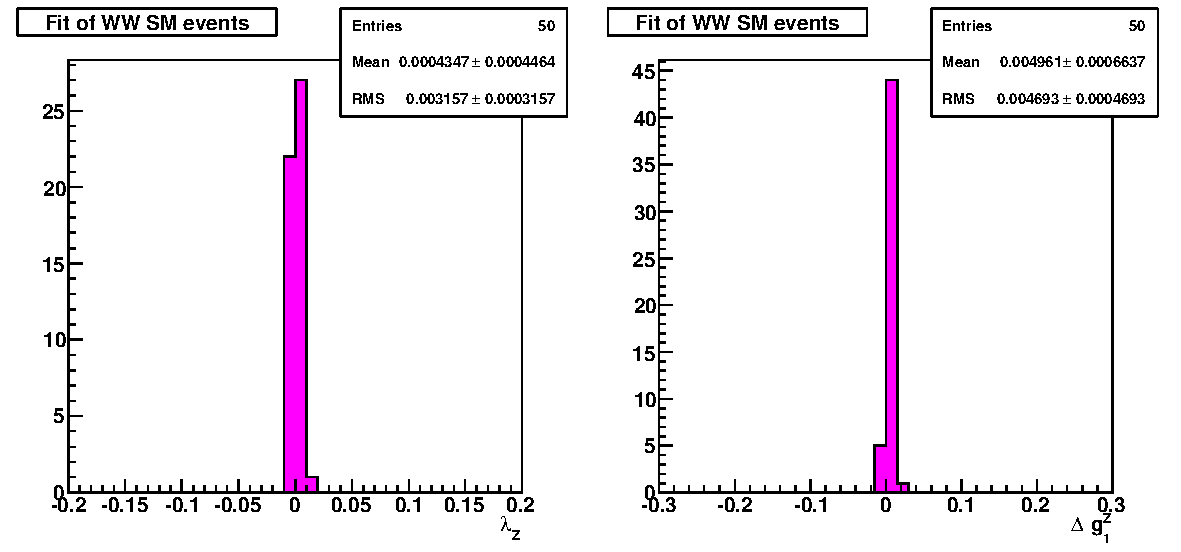
\includegraphics[width=1.0\textwidth]{figures/fit_ww_mc_1D}
    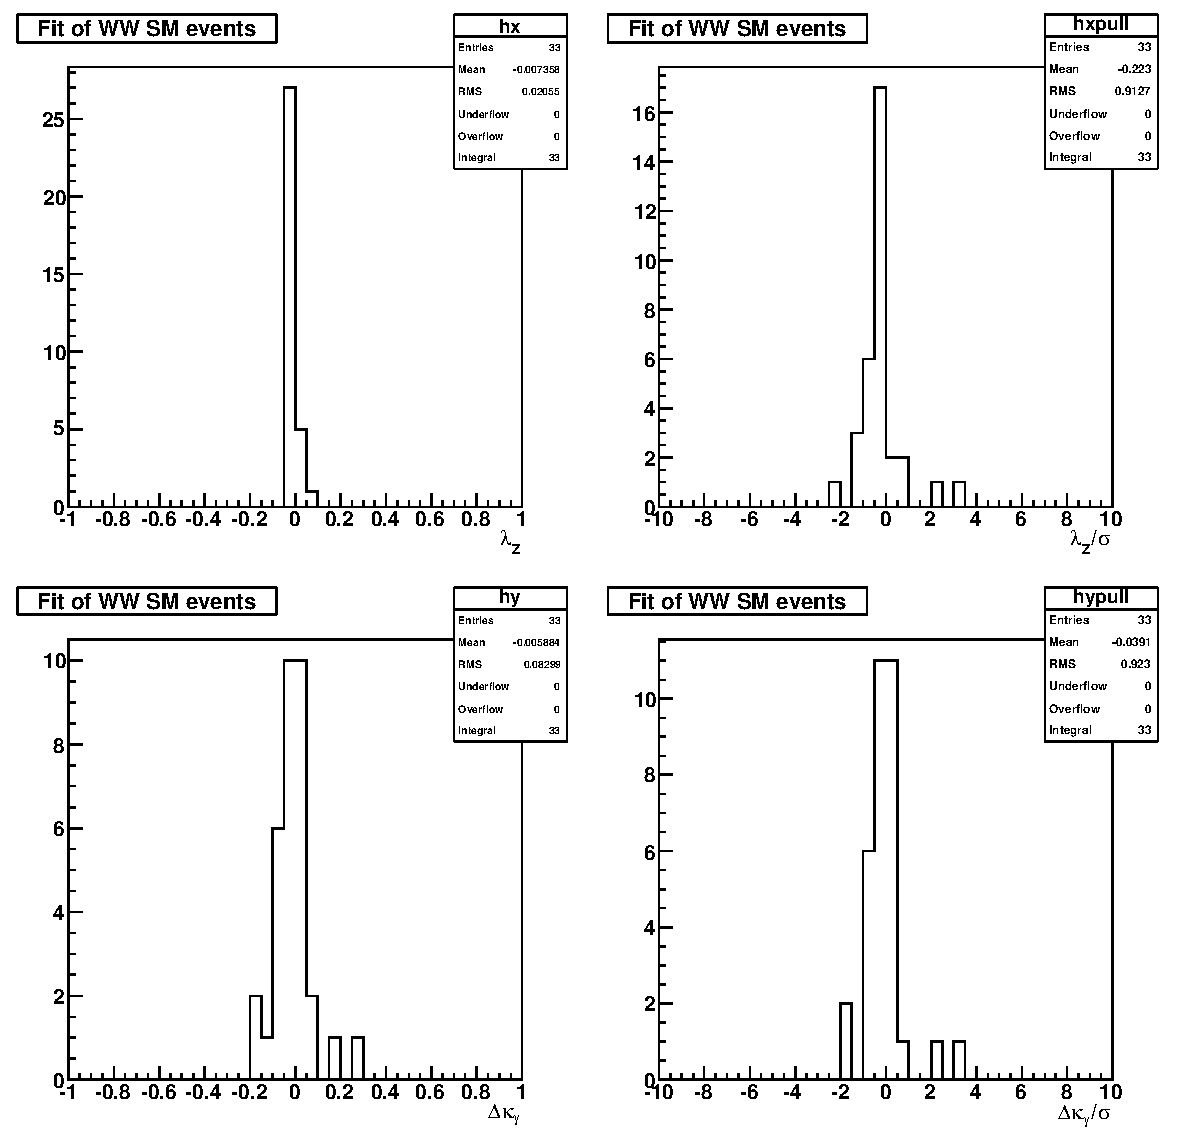
\includegraphics[width=1.0\textwidth]{figures/fit_ww_mc_1D_2}

  \caption[1D fits to WW SM Monte Carlo] {Fit results for
  2-dimentional $\lambda_{Z}$-$\Delta g^Z_1$ (top) and
  $\lambda_{Z}$-$\Delta\kappa_\gamma$ (bottom) aTGC models using 50
  independent pseudo-data experiments made of Madgraph Standard
  Model \ww\ simulated data. Only one coupling floating in the fit,
  while the other one is fixed to the Standard Model
  value. Backgrounds are excluded from the fits.}

\label{fig:fit_ww_mc_1D}
\end{figure}


%% \begin{figure}[tp]
%%   \centerline{
%%     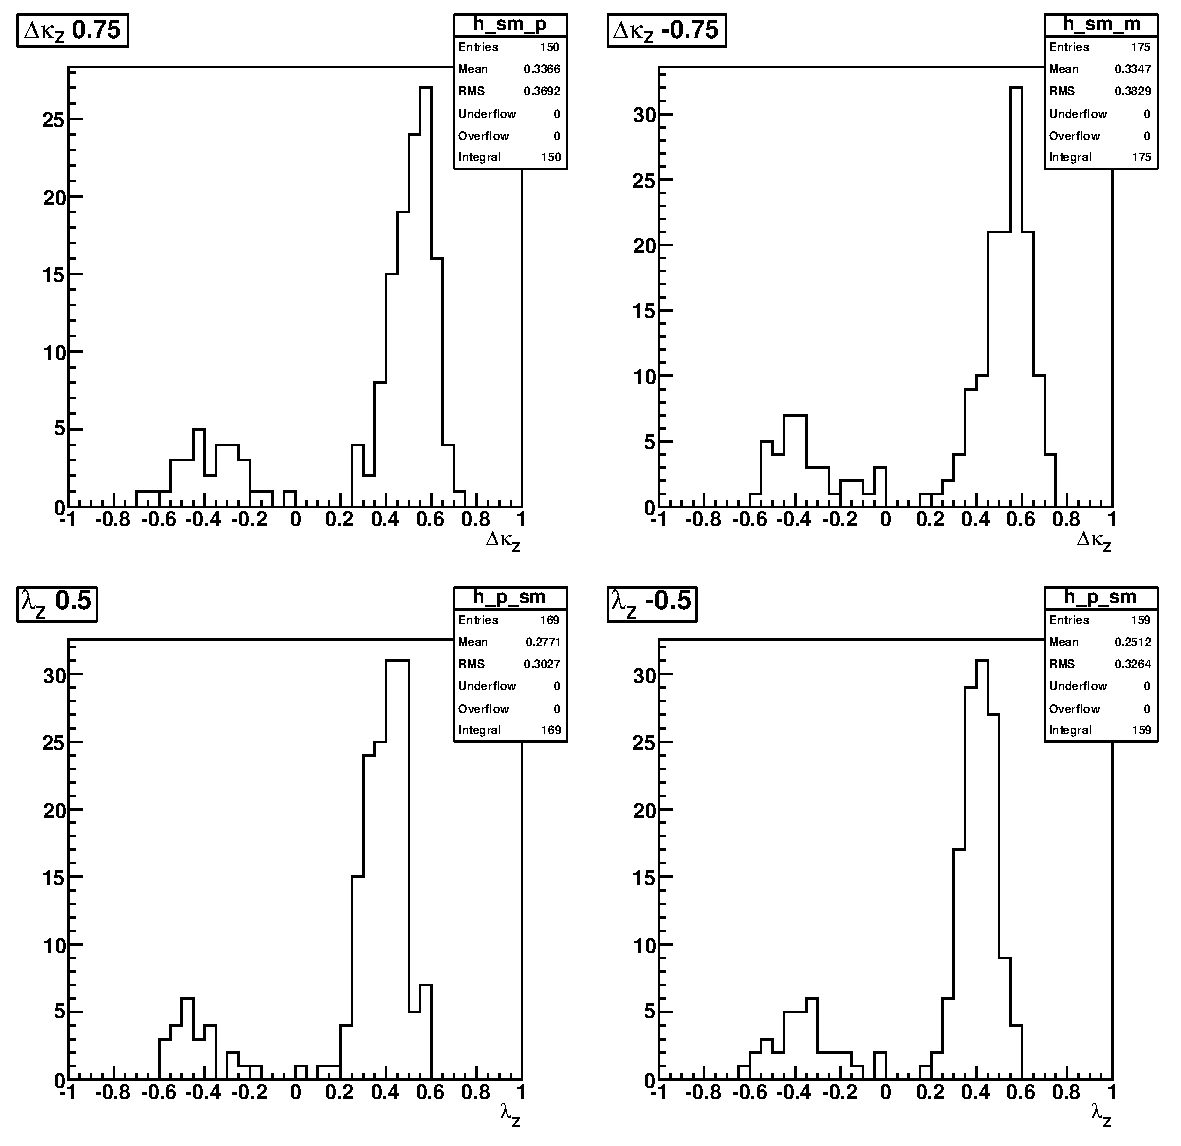
\includegraphics[width=1.0\textwidth]{figures/fit_wwATGC_mc_1D_pm}
%%   }

%%   \caption[1D fits to WW aTGC Monte Carlo] {Fits to WW Monte Carlo
%%     samples with anomalous couplings with 11 events in a sample. No
%%     background. Only one coupling is floated in the fit. Sign of the
%%     coupling cannot be determined in the fit.}
%%   \label{fig:fit_wwATGC_mc_1D_pm}
%% \end{figure}

\begin{figure}[tp]
  \centering
    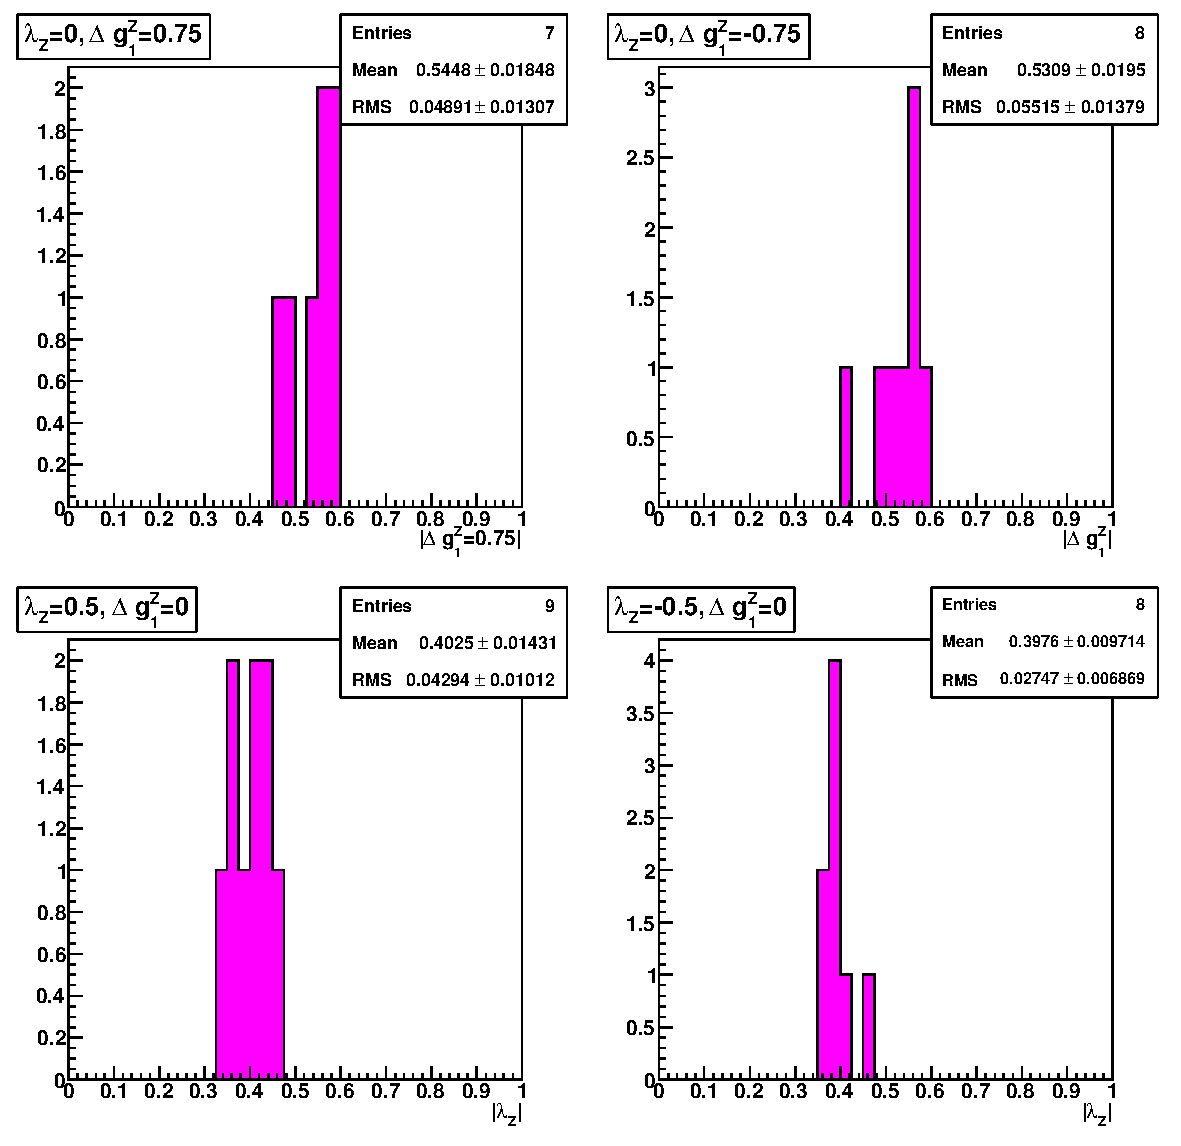
\includegraphics[width=0.8\textwidth]{figures/fit_wwATGC_mc_1D_abs}
    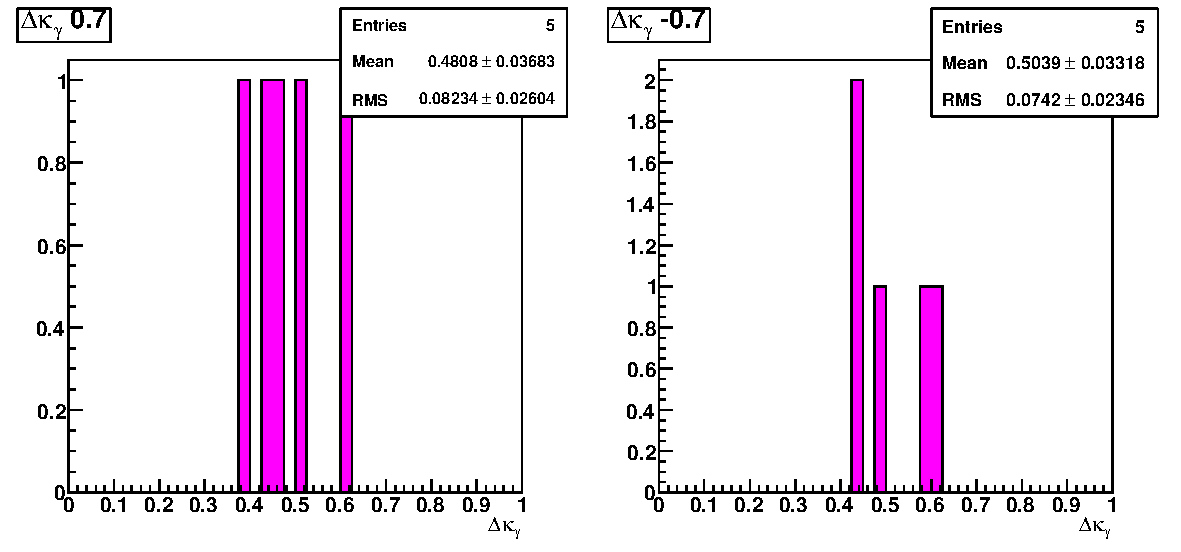
\includegraphics[width=0.8\textwidth]{figures/fit_wwATGC_mc_1D_abs2}

  \caption[1D fits to WW aTGC Monte Carlo] {Fits to $WW$ Monte Carlo
    samples with anomalous couplings. Pseudo-data experiments are made
    with 5-10 times lower number of events in each experiment due
    limited amount of simulated data. Backgrounds are excluded from
    the fits. Only one coupling is allowed to float in the
    fit. Absolute values of the couplings are  shown.}  
    \label{fig:fit_wwATGC_mc_1D_abs}
\end{figure}

\subsection{Fit on data}
We check how much the normalization of different components were
changed during the fit with respect to the inial values. For this test
we treat anomalous couplings as nuisance parameters and hide their
central values.

Table~\ref{tab:fit_yields} summarizes the fit results for event
yields. From it we conclude that the excess of the events that we
observed in the cross-section measurement is absorbed mostly
in \wjets~ event yield. Looking at the correlation matrix
Figure~\ref{fig:fit_correlations} one can see that there is
significant correlation between \wjets~ and \ww~ event yields. Small
mis-modeling of the low pt part of the leading lepton distribution may
cause the excess to be split between the two contributions. This
effect has no impact on the anomalous coupling measurement, since it
mostly sensitive to the excess of events at high \pt{}. 

As a cross-check we performed a fit fixing the \wjets\ yield to its
estimate and keeping it constant. The excess was mostly absorbed
by \ww normalization. The impact on measured anomalous couplings was
less than 0.0006, i.e. totally negligible at the current level of
sensitivity.

%% Minuit2Minimizer: Minimize with max iterations 4000 edmval 1 strategy 1
%% Minuit2Minimizer : Valid minimum - status = 0
%% FVAL  = -1602.82913488348504
%% Edm   = 5.45511397378936264e-05
%% Nfcn  = 134
%% n_dy      = 15.9038    +/-  6.61673     (limited)
%% n_top     = 124.086    +/-  20.9979     (limited)
%% n_wjets   = 125.501    +/-  20.314      (limited)
%% n_ww      = 817.58     +/-  46.044      (limited)
%% n_wz      = 19.0359    +/-  1.89804     (limited)
%% n_zz      = 10.6562    +/-  0.999016    (limited)
%% x_par     = 0.00151822 +/-  0.0190978   (limited)
%% y_par     = 0.00503943 +/-  0.0304233   (limited)
%% Minos: Lower error for parameter 0  :  -6.74416
%% Minos: Upper error for parameter 0  :  6.74374
%% Minos: Lower error for parameter 1  :  -20.8847
%% Minos: Upper error for parameter 1  :  21.2024
%% Minos: Lower error for parameter 2  :  -20.2856
%% Minos: Upper error for parameter 2  :  20.4984
%% Minos: Lower error for parameter 3  :  -46.2509
%% Minos: Upper error for parameter 3  :  45.9041
%% Minos: Lower error for parameter 4  :  -1.89954
%% Minos: Upper error for parameter 4  :  1.89966
%% Minos: Lower error for parameter 5  :  -0.999735
%% Minos: Upper error for parameter 5  :  0.999722
%% Minos: Lower error for parameter 6  :  -0.0189644
%% Minos: Upper error for parameter 6  :  0.0182371
%% Minos: Lower error for parameter 7  :  -0.0301162
%% Minos: Upper error for parameter 7  :  0.0295189
%%
%%   RooFitResult: minimized FCN value: -1602.83, estimated distance to minimum: 2.12194e-05
%%                 covariance matrix quality: Full, accurate covariance matrix
%%
%%     Floating Parameter  InitialValue    FinalValue +/-  Error     GblCorr.
%%   --------------------  ------------  --------------------------  --------
%%                   n_dy    1.5909e+01    1.5909e+01 +/-  6.62e+00  0.215534
%%                  n_top    1.2416e+02    1.2416e+02 +/-  2.10e+01  0.522827
%%                n_wjets    1.2557e+02    1.2557e+02 +/-  2.03e+01  0.547777
%%                   n_ww    8.1733e+02    8.1733e+02 +/-  4.61e+01  0.687014
%%                   n_wz    1.9036e+01    1.9036e+01 +/-  1.90e+00  0.063578
%%                   n_zz    1.0656e+01    1.0656e+01 +/-  9.99e-01  0.031781
%%                  x_par    1.5155e-03    1.5155e-03 +/-  1.91e-02  0.113013
%%                  y_par    5.0221e-03    5.0221e-03 +/-  3.04e-02  0.121154


\begin{table}[!ht]
  \begin{center}
 {\small
  \begin{tabular} {|l|c|c|c|}
\hline
  Parameter       &   Initial value & Fit value & Global Correlation \\
\hline
  N$_{\ww}$       & $819.9\pm57.6$  & $817.6\pm46.0$ & 0.69 \\
  N$_{Top}$       & $121.6\pm23.4$  & $124.1\pm21.0$ & 0.52 \\
  N$_{\wjets}$    & $78.1\pm22.0$   & $125.6\pm20.3$ & 0.55 \\
  N$_{\wz}$       & $18.5\pm1.9$    & $19.0\pm1.9$   & 0.06 \\
  N$_{\dyll}$     & $11.7\pm6.8$    & $15.9\pm6.6$   & 0.22 \\
  N$_{\zz}$       & $10.6\pm1.0$    & $10.7\pm1.0$   & 0.03 \\
\hline
  \end{tabular}
  }
  \caption{Nominal fit parameter values.}
   \label{tab:fit_yields}
  \end{center}
\end{table}

\begin{figure}[tp]
  \centerline{
    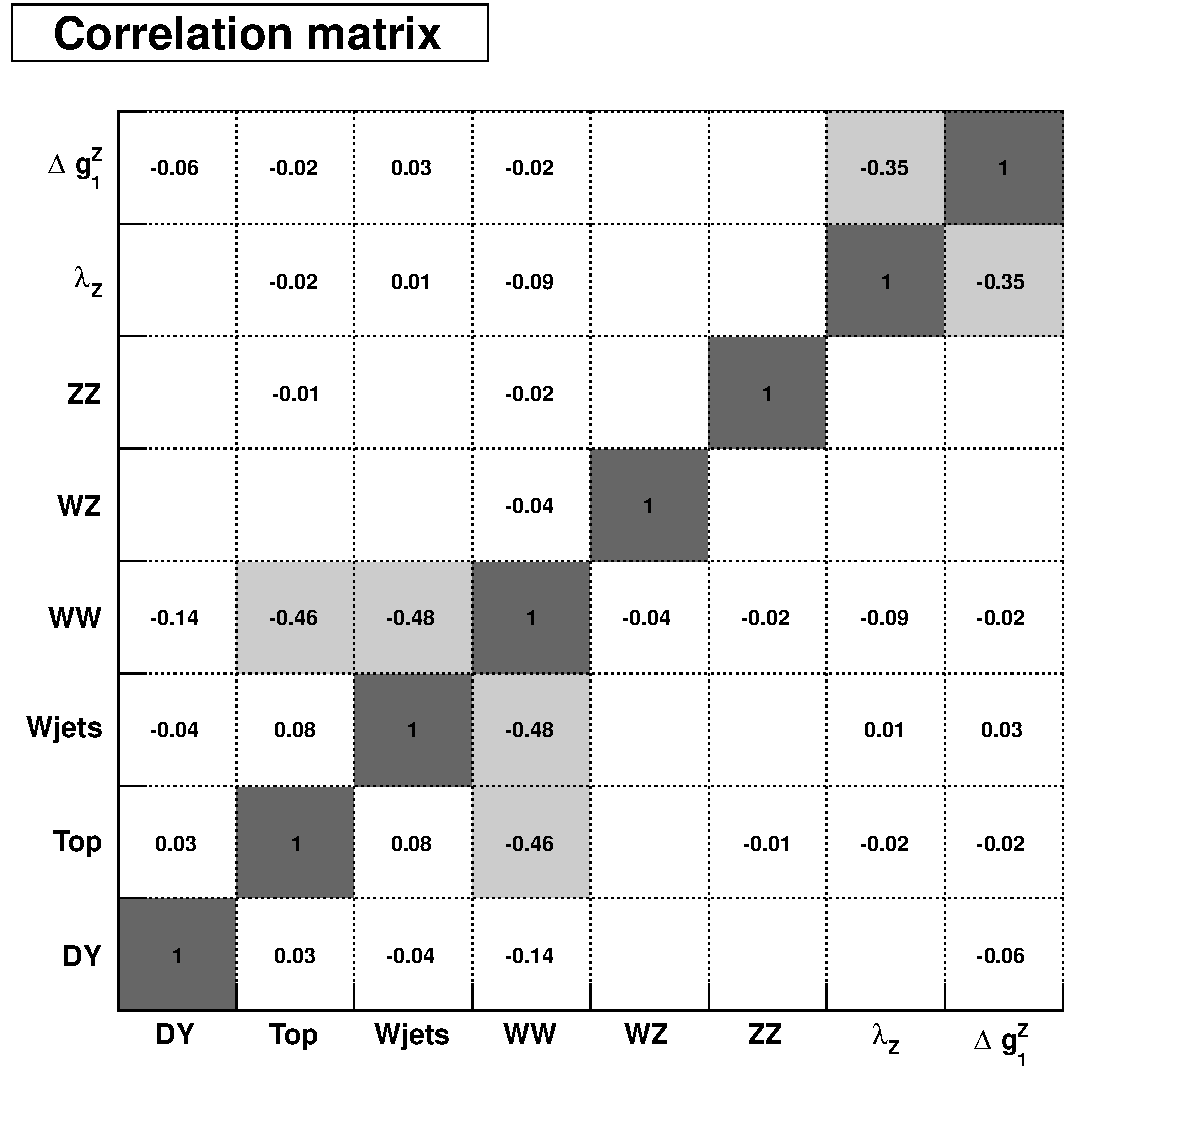
\includegraphics[width=.45\textwidth]{figures/correlations}
  }

  \caption[Fit parameter correlations] {Correlation matrix for the nominal fit parameters.}
  \label{fig:fit_correlations}
\end{figure}

\clearpage
\section{Results}
   \label{sec:results}
   \subsection{Statistical Methods}
We derive upper limits on the product of the Higgs boson production
cross section and the $\Hi \to \WW$ branching fraction,
$\sigma_{\rm{H}} \times $BR($\Hi \to \WW)$, with respect to the SM
expectation, i.e. $\sigma^{95\%}/\sigma^{SM}$. Two different
statistical methods are used to report results. The first method is
based on Bayesian inference~\cite{bayesian} and the second one, known
as $CL_{s}$, is the modified frequentist approach~\cite{cls1,cls2}.

The likelihood function is defined as:
\begin{eqnarray}
  L(\rm{data}|\mu,\theta)&=&\rm{Poisson}(\rm{data}|\mu\cdot s(\theta)+b(\theta))\cdot p(\tilde{\theta}|\theta) \nonumber\\
 &=&\prod_i\frac{(\mu s_i+b_i)^{n_i}}{n_i!}e^{-\mu s_i-b_i}\cdot p(\tilde{\theta}|\theta)
\label{eq:likelihood}
\end{eqnarray}
where $\mu$ is the signal strength modifier which is often reported in
the upper limit results as a ratio of the cross-section upper limit
over the standard model cross-section and $\theta$ represents a full
set of nuisance parameters that are used to incorporate systematic
uncertainties. 

The first method (Bayesian) is based on interpreting the likelihood
(Eq.~\ref{eq:likelihood}) as a probability distribution function with
a flat prior for the signal strength and a set of pdfs for nuisance
parameters, which are often approximated with the log-normal
distribution. Integrating over the nuisance parameters we find the
upper limit for the signal strength.

For $CL_{s}$ method the test statistic is defined as a likelihood
ratio:
\begin{equation}
\tilde{q_\mu}=-2\log\frac{L(\rm{data}|\mu,\hat\theta_\mu)}{L(\rm{data}|\hat\mu,\hat\theta)}
\end{equation}
where the numerator corresponds to the maximum likelihood for given
``data'' and $\mu$ profiling over the nuisance parameters and the
denominator corresponds to the maximum likelihood for given ``data''
profiling over the nuisance parameters and $\mu$. This test statistic
differs from the ones used at LEP (no profiling of systematic errors)
and at Tevatron (the denominator likelihood uses $\mu=0$ and only
systematic errors are profiled).

The results obtained using the two methods may differ but in most cases
they are very close. To perform the computation of the limits, the
software packages
\texttt{RooStats}~\cite{rootstat} and \texttt{LandS}~\cite{lands} have 
been used.

\subsection{Background Estimation}

The estimation of the backgrounds follows the strategies described in
Section~\ref{sec:backgrounds}. As mentioned at the begining of the 
document, we are totally/partially missing $\wgamma$, $\wgamma^{*}$ and $\WZ$
in simulation. Thus, Monte Carlo yields and data/MC scale factors 
are preliminary.

First we estimate the $\dyll$ at the WW selection level shown in Table~\ref{tab:dy_wwlevel}. 
As it was seen before the simulation significantly underestimates this type of
background. It is important to keep in mind that $\WZ$ and $\ZZ$ 
contributions in the $\Z$-peak region are sizable, so the method depends
on the Monte Carlo simulation of these processes. It is not a problem
since the uncertainties on these di-boson contributions in the Z-peak
region are small compared with the systematic uncertainties of the
R-value extraction and the statistical uncertainties on the number of
the events in Z-peak region.
As we do not have enough statistics in the MC at the higgs selection level, 
we estimate directly at the Higgs selection level for both the 
cut-based and shape-based analyses. 
The results are shown in Table~\ref{tab:dy}. 

The $\Wjets$ background contribution is summarized in Table~\ref{tab:fake_est}. 
The same sign closure test in the 0-jet bin finds 276 events in data while 
the background expectation is $310 \pm 10~(stat.)$.

The top background estimation is shown in
Table~\ref{tab:ttbar_est}. The scale factors are consistent with unity within 
the current large statistical uncertainties. 

With these results, we compare the yields after the $\WW$ preselection 
in data and MC with min-MET(Table~\ref{tab:wwselection_all_minmet}) and 
DY MVA(Table~\ref{tab:wwselection_all_dymva}). Higgs contribution at
\WW\ selection level is negligible for not excluded Higgs mass
hypotheses. For the signal extraction we estimate the \WW\ background
contribution in data looking at events with large di-lepton mass, i.e.
$m_{ll}>100$~\GeV{} (Table~\ref{tab:ww_est}). 
Figures~\ref{fig:ww_ptmax}-\ref{fig:ww_deltaphi} show a few key distributions at \WW\ selection level.

%%%%%%%%%%%%%%%%%%%%%%%%%%%%%%
\begin{table}
\begin{center}
\begin{tabular}{c c c c c c}
\hline
       nJets & $N_{in}$(data)        & $R_{out/in}$        & $N_{out}$(data)  & $N_{out}$ (MC) \\ 
0 & $417.2\pm50.4$ 		& $0.27\pm0.01\pm0.02$ & $114.1\pm14.8\pm8.5$ 	& $18.97\pm5.59$ 	\\
1 & $191.8\pm27.4$ 		& $0.22\pm0.01\pm0.07$ & $43.0\pm6.4\pm13.0$ 	& $13.54\pm4.66$  \\
2 & $1964.4\pm48.9$ 	& $0.26\pm0.01\pm0.03$ & $507.0\pm21.0\pm53.9$ & $260.93\pm19.94$  \\
\hline
\end{tabular}
\caption{The Drell-Yan estimation in the same flavor final state at WW preselection level, using the DYMVA in 
0 and 1 Jet bins and the pfMET at the 2-jet bins. }
\label{tab:dy_wwlevel}
\end{center}
\end{table}

%%%%%%%%%%%%%%%%%%%%%%%%%%%%%%
\begin{table}
\begin{center}
\begin{tabular}{c c c c c c}
\hline
\hline
\multicolumn{5}{c}{0-jet} \\
\hline
mass & $N_{in}$(data)        & $R_{out/in}$        & $N_{out}$(data)  & $N_{out}$ (MC) \\ 
\hline
115 \GeV &$ 78.9\pm11.5 $&$ 0.32\pm0.02\pm0.08 $&$ 24.9\pm3.9\pm6.4 $&$ 6.06\pm3.59 $\\
120 \GeV &$ 129.2\pm15.6 $&$ 0.32\pm0.02\pm0.08 $&$ 40.7\pm5.5\pm10.5 $&$ 10.31\pm4.30 $\\
125 \GeV &$ 83.0\pm12.4 $&$ 0.62\pm0.04\pm0.12 $&$ 51.7\pm8.5\pm10.0 $&$ 10.31\pm4.30 $\\
130 \GeV &$ 64.1\pm11.0 $&$ 0.87\pm0.06\pm0.15 $&$ 56.1\pm10.4\pm9.7 $&$ 10.31\pm4.30 $\\
135 \GeV &$ 59.5\pm11.1 $&$ 0.82\pm0.06\pm0.12 $&$ 48.9\pm9.8\pm7.4 $&$ 8.71\pm3.99 $\\
140 \GeV &$ 59.2\pm11.1 $&$ 0.78\pm0.06\pm0.09 $&$ 46.0\pm9.3\pm5.1 $&$ 8.71\pm3.99 $\\
145 \GeV &$ 59.2\pm11.1 $&$ 0.78\pm0.06\pm0.09 $&$ 46.0\pm9.3\pm5.1 $&$ 8.71\pm3.99 $\\
150 \GeV &$ 44.2\pm11.2 $&$ 0.30\pm0.04\pm0.19 $&$ 13.5\pm3.9\pm8.3 $&$ 1.07\pm1.07 $\\
160 \GeV &$ 12.8\pm6.8 $&$ 0.79\pm0.14\pm0.37 $&$ 10.1\pm5.6\pm4.8 $&$ 1.07\pm1.07 $\\
170 \GeV &$ 3.5\pm6.2 $&$ 0.68\pm0.13\pm0.59 $&$ 2.4\pm4.2\pm2.0 $&$ 1.07\pm1.07 $\\
180 \GeV &$ 3.5\pm7.4 $&$ 0.52\pm0.09\pm0.09 $&$ 1.8\pm3.8\pm0.3 $&$ 0.00\pm0.00 $\\
190 \GeV &$ 23.7\pm11.5 $&$ 0.28\pm0.04\pm0.05 $&$ 6.6\pm3.3\pm1.1 $&$ 1.36\pm1.36 $\\
200 \GeV &$ 34.2\pm15.8 $&$ 0.18\pm0.03\pm0.03 $&$ 6.2\pm3.0\pm0.9 $&$ 1.36\pm1.36 $\\
250 \GeV &$ 87.4\pm25.4 $&$ 0.05\pm0.01\pm0.01 $&$ 4.0\pm1.3\pm1.1 $&$ 4.63\pm2.68 $\\
300 \GeV &$ 32.3\pm19.3 $&$ 0.09\pm0.02\pm0.20 $&$ 3.0\pm1.9\pm6.3 $&$ 4.63\pm2.68 $\\
\vspace{-3mm}  \\
\hline
\hline
\multicolumn{5}{c}{1-jet} \\
\hline
mass & $N_{in}$(data)        & $R_{out/in}$        & $N_{out}$(data)  & $N_{out}$ (MC) \\ 
\hline
115 \GeV &$ 19.2\pm6.7 $&$ 0.16\pm0.01\pm0.03 $&$ 3.0\pm1.1\pm0.5  $&$ 0.00\pm0.00 $\\
120 \GeV &$ 42.8\pm9.3 $&$ 0.16\pm0.01\pm0.03 $&$ 6.7\pm1.5\pm1.2  $&$ 0.00\pm0.00 $\\
125 \GeV &$ 32.8\pm7.9 $&$ 0.23\pm0.01\pm0.04 $&$ 7.5\pm1.9\pm1.3  $&$ 0.00\pm0.00 $\\
130 \GeV &$ 30.5\pm7.3 $&$ 0.30\pm0.02\pm0.05 $&$ 9.1\pm2.3\pm1.6  $&$ 0.00\pm0.00 $\\
135 \GeV &$ 29.7\pm7.6 $&$ 0.28\pm0.02\pm0.04 $&$ 8.2\pm2.2\pm1.3  $&$ 0.00\pm0.00 $\\
140 \GeV &$ 27.3\pm7.6 $&$ 0.25\pm0.02\pm0.05 $&$ 6.9\pm2.0\pm1.3  $&$ 0.00\pm0.00 $\\
145 \GeV &$ 27.3\pm7.6 $&$ 0.25\pm0.02\pm0.05 $&$ 6.9\pm2.0\pm1.3  $&$ 0.00\pm0.00 $\\
150 \GeV &$ 35.6\pm9.2 $&$ 0.16\pm0.01\pm0.04 $&$ 5.9\pm1.6\pm1.4  $&$ 0.00\pm0.00 $\\
160 \GeV &$ 12.8\pm4.9 $&$ 0.37\pm0.04\pm0.14 $&$ 4.8\pm1.9\pm1.9  $&$ 0.00\pm0.00 $\\
170 \GeV &$ 13.9\pm5.3 $&$ 0.34\pm0.04\pm0.12 $&$ 4.8\pm1.9\pm1.7  $&$ 0.00\pm0.00 $\\
180 \GeV &$ 14.2\pm5.9 $&$ 0.28\pm0.03\pm0.09 $&$ 4.0\pm1.7\pm1.3  $&$ 0.00\pm0.00 $\\
190 \GeV &$ 44.0\pm10.4 $&$ 0.21\pm0.02\pm0.04 $&$ 9.1\pm2.3\pm1.9  $&$ 0.00\pm0.00 $\\
200 \GeV &$ 59.2\pm12.6 $&$ 0.16\pm0.01\pm0.03 $&$ 9.5\pm2.1\pm1.7  $&$ 0.00\pm0.00 $\\
250 \GeV &$ 71.0\pm16.2 $&$ 0.09\pm0.01\pm0.00 $&$ 6.2\pm1.5\pm0.2  $&$ 1.62\pm1.62 $\\
300 \GeV &$ 40.2\pm13.2 $&$ 0.09\pm0.01\pm0.02 $&$ 3.8\pm1.3\pm0.9  $&$ 3.12\pm2.21 $\\
\vspace{-3mm}  \\
\hline
\hline
\multicolumn{5}{c}{2-jet} \\
\hline
mass & $N_{in}$(data)        & $R_{out/in}$        & $N_{out}$(data)  & $N_{out}$ (MC) \\
\hline
115 \GeV &$ 6.93\pm2.65 $&$ 0.25\pm0.06\pm0.11 $&$ 1.72\pm0.79\pm0.77 $&$ 2.17\pm1.58 $	\\
120 \GeV &$ 12.88\pm3.61 $&$ 0.25\pm0.06\pm0.11 $&$ 3.20\pm1.21\pm1.42 $&$ 2.17\pm1.58$	\\
125 \GeV &$ 6.90\pm2.65 $&$ 0.35\pm0.09\pm0.16 $&$ 2.40\pm1.11\pm1.07 $&$ 2.17\pm1.58$	\\
130 \GeV &$ 5.94\pm2.45 $&$ 0.47\pm0.13\pm0.12 $&$ 2.78\pm1.37\pm0.70 $&$ 2.17\pm1.58$	\\
135 \GeV &$ 7.94\pm2.83 $&$ 0.45\pm0.12\pm0.24 $&$ 3.54\pm1.59\pm1.94 $&$ 2.17\pm1.58$	\\
140 \GeV &$ 7.94\pm2.83 $&$ 0.48\pm0.13\pm0.28 $&$ 3.80\pm1.72\pm2.21 $&$ 0.81\pm0.81$	\\
145 \GeV &$ 7.94\pm2.83 $&$ 0.48\pm0.13\pm0.28 $&$ 3.80\pm1.72\pm2.21 $&$ 0.81\pm0.81$	\\
150 \GeV &$ 11.84\pm3.75 $&$ 0.27\pm0.10\pm0.17 $&$ 3.22\pm1.54\pm2.04 $&$ 0.00\pm0.00$	\\
160 \GeV &$ 4.95\pm2.24 $&$ 0.76\pm0.34\pm0.62 $&$ 3.76\pm2.38\pm3.05 $&$ 0.00\pm0.00$	\\
170 \GeV &$ 6.94\pm2.65 $&$ 0.76\pm0.34\pm0.76 $&$ 5.26\pm3.08\pm5.26 $&$ 0.00\pm0.00$ \\
180 \GeV &$ 10.83\pm3.61 $&$ 0.45\pm0.18\pm0.45 $&$ 4.91\pm2.57\pm4.91 $&$ 0.00\pm0.00$ \\
190 \GeV &$ 18.68\pm4.80 $&$ 0.33\pm0.11\pm0.33 $&$ 6.09\pm2.57\pm6.09 $&$ 0.00\pm0.00$ \\
200 \GeV &$ 19.56\pm4.91 $&$ 0.22\pm0.07\pm0.22 $&$ 4.32\pm1.81\pm4.32 $&$ 0.00\pm0.00$ \\
250 \GeV &$ 34.14\pm6.25 $&$ 0.15\pm0.05\pm0.15 $&$ 5.19\pm2.01\pm5.19 $&$ 0.00\pm0.00$ \\
300 \GeV &$ 25.27\pm5.67 $&$ 0.09\pm0.06\pm0.09 $&$ 2.26\pm1.52\pm2.26 $&$ 0.00\pm0.00$ \\
\hline 
\hline
\end{tabular}
\caption{The Drell-Yan estimation in the same flavor final state, for the cut-based selections.}
\label{tab:dy}
\end{center}
\end{table}

%%%%%%%%%%%%%%%%%%%%%%%%%%%%%% 
\begin{table}[ht!]
\begin{center}
\begin{tabular}{c c c c c c} 
\hline
jet-bin &	 $\mu\mu$ &	 $e \mu$ &	 $\mu e$ &	 $ee$ &	 total \\ 
\hline
0 &  67.65 +/-  7.10   &  58.88 +/-  4.56     &  199.91 +/-  8.27  & 46.74 +/-  2.49  & 373.19 +/- 12.08 \\
1 &  44.31 +/-  6.16   &  61.31 +/-  5.38     &  178.08 +/-  8.25  & 18.07 +/-  1.75  & 301.78 +/- 11.75 \\ 
2 &  46.44 +/-  7.69   &  35.34 +/-  4.63     &  118.47 +/-  7.39  & 15.93 +/-  1.67  & 216.20 +/- 11.75 \\ 
\hline
\end{tabular}
\caption{Predictions of the fake-induced background contribution 
in the data-driven estimation after the $\WW$ preselection. 
The analyzed data correspond to $\intlumiEightTeV$, where the reported uncertainties are statistical only.}
\label{tab:fake_est}
\end{center}
\end{table}
%%%%%%%%%%%%%%%%%%%%%%%%%%%%%%
\begin{table}[ht!]
\begin{center}
\begin{tabular}{l c c c}
\hline
                                   Sample & 0-jet           & 1-jet           & 2-jet       \\
\hline
estimated top events in simulation  & 423.1 $\pm$   2.7 &  1312.0 $\pm$   9.0 &  31.7 $\pm$   1.3 \\
tagging efficiency     (\%)         & 49.4 $\pm$  4.3 & 65.1 $\pm$  0.6 & - \\ 
data events in control region       &  599 & 2997 & - \\ 
background events in control region & 191.4 $\pm$  28.7 &  189.8 $\pm$  38.0 & - \\ 
top estimation in data              &  417.9 $\pm$  85.7 &  1425.4 $\pm$  46.5 &   4.2 $\pm$   3.0 \\
data/simulation scale factor        &   0.99 $\pm$  0.20 &   1.09 $\pm$  0.04 &  1.02 $\pm$  0.25 \\
\hline
\end{tabular}
\caption{Monte Carlo to data scale factor for the top background contribution for $\intlumiEightTeV$. 
In the 1-jet bin, the scale factor is derived in a region that is slightly different from the signal region.}
\label{tab:ttbar_est}
\end{center}
\end{table}
%%%%%%%%%%%%%%%%%%%%%%%%%%%%%%

\begin{table}[ht!]
  \begin{center}
 {\small
  \begin{tabular} {|c|c|c|c|c|c|c|}
\hline
          &   data & all bkg. & $qq \to \WW$ & $gg \to \WW$ &  $\ttbar+tW$   & $\Wjets$    \\
  \hline
  \hline
%	0-jet	&   1594 & 1320.41 $\pm$ 15.49 &   853.83  $\pm$  6.17 & 51.96 $\pm$  1.13 &  160.48 $\pm$  5.41  & 151.12 $\pm$  6.69  \\	   
%	1-jet	&   1171 & 1159.81 $\pm$ 15.92 &   391.48  $\pm$  4.22 & 21.32 $\pm$  0.73 &  526.30 $\pm$  8.04  & 108.05 $\pm$  6.71  \\   
	0-jet	&   4416 & ?  &   2478.31 $\pm$ 10.20  & 160.86 $\pm$ 1.94 &  415.74 $\pm$ 7.77  & 371.04 $\pm$ 12.09  \\	   
 \hline
 \hline
  \end{tabular}
  \begin{tabular} {|c|c|c|c|c|}
\hline
       & $WZ$/$ZZ$ not included in the $\dyll$ & $\dyll+WZ+ZZ$ & $W+\gamma$ \\
  \hline
  \hline
%	0-jet 	&  23.36 $\pm$  0.42 & 51.82 $\pm$ 10.64 & 27.84 $\pm$  3.62 \\ 
%	1-jet 	&  26.39 $\pm$  0.45 & 66.10 $\pm$ 10.51 & 20.17 $\pm$  3.83 \\
	0-jet 	&  96.90 $\pm$ 1.26  & 56.38 $\pm$ 2.96 & 131.48 $\pm$ 10.44  \\ 
 \hline
 \hline
  \end{tabular}
  }
  \caption{\fixme Expected number of signal and background events from the data-driven methods for 
  an integrated luminosity of \intlumiEightTeV after applying the $\WW$ selection requirements. 
  Only statistical uncertainties on the processes are reported. $\WW$ yield is from MC.}
   \label{tab:wwselection_all_dymva}
  \end{center}
\end{table}
%%%%%%%%%%%%%%%%%%%%%%%%%%%%%%%%%%%%

\begin{figure}[!hbtp]
\centering
\subfigure[]{
\centering
\label{subfig:ww_ptmin_0j}
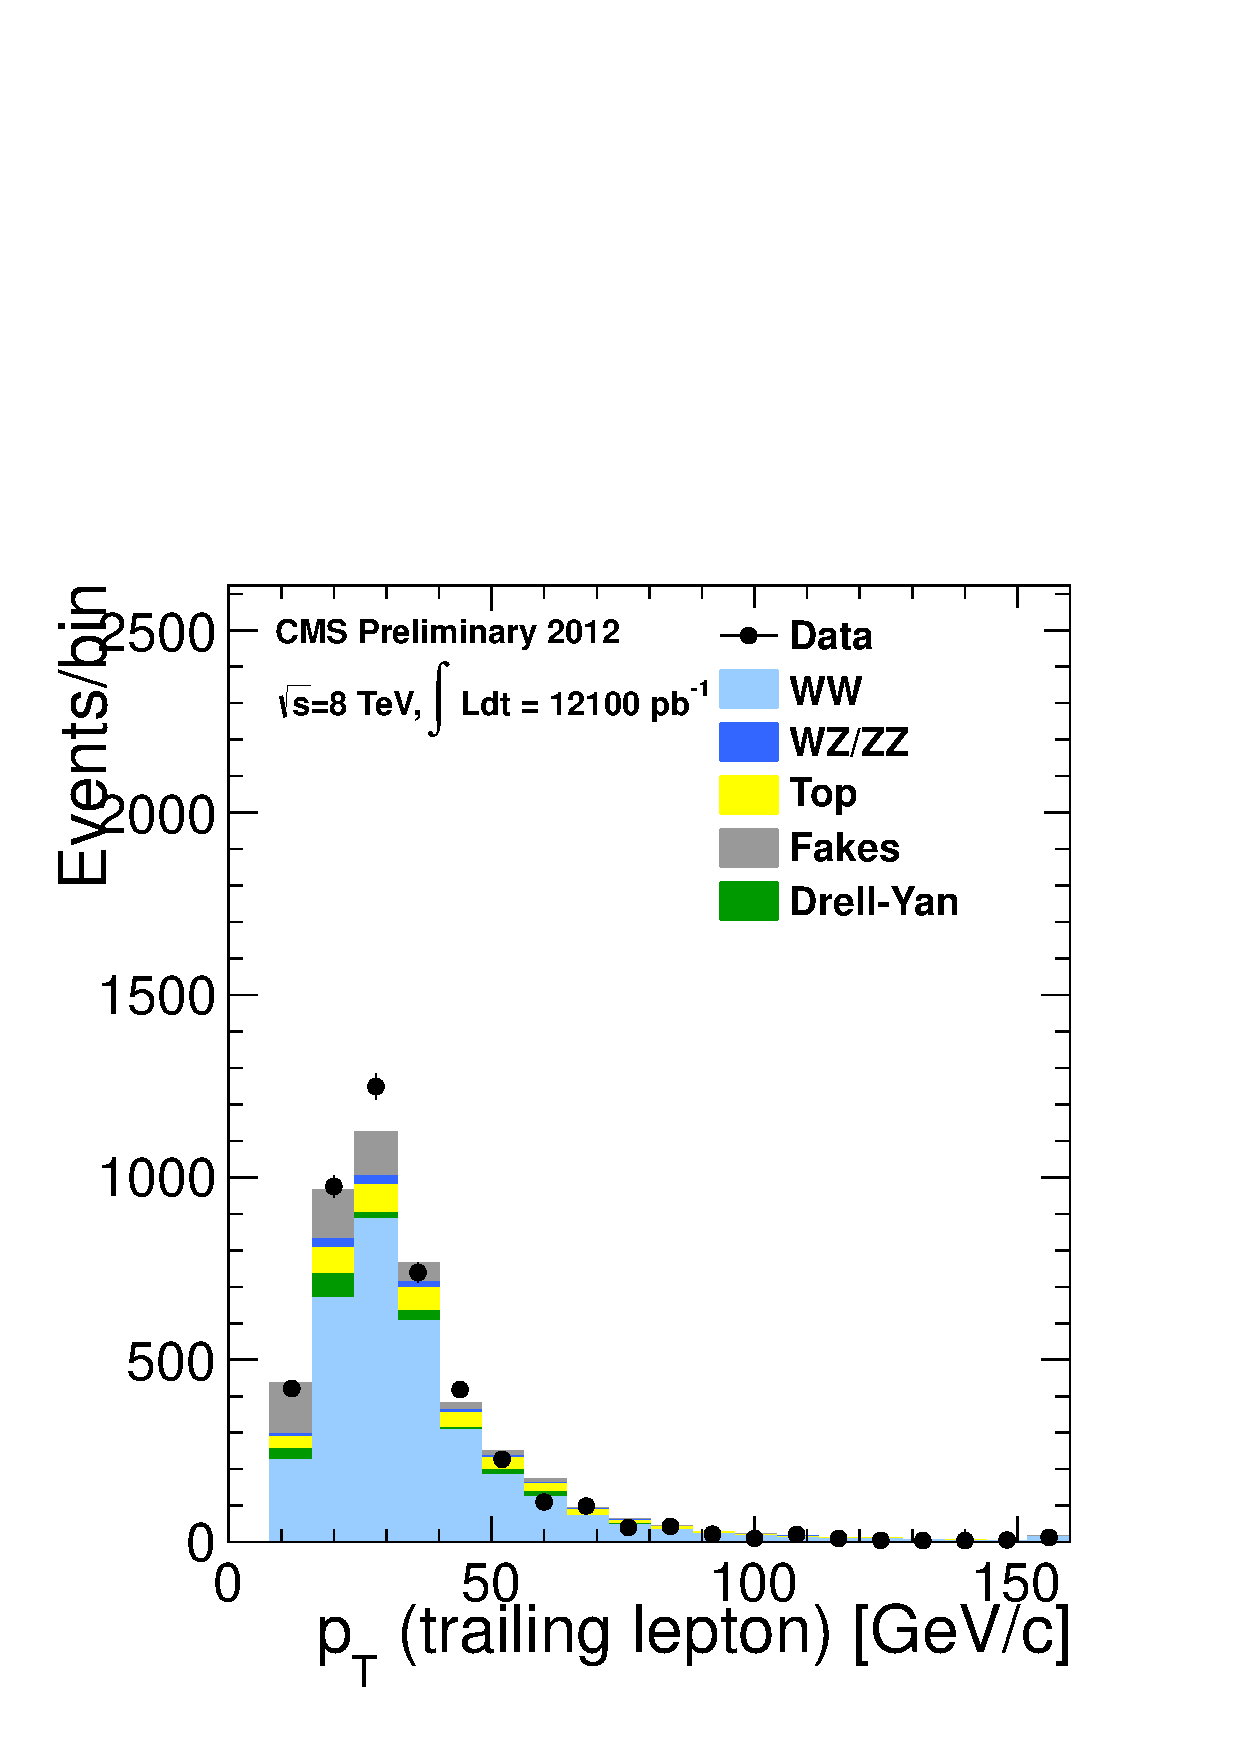
\includegraphics[width=.3\textwidth]{figures/hww_analysis16_0_ALL_incl_0j_pt2.pdf}
}
\subfigure[]{
\centering
\label{subfig:ww_ptmin_1j}
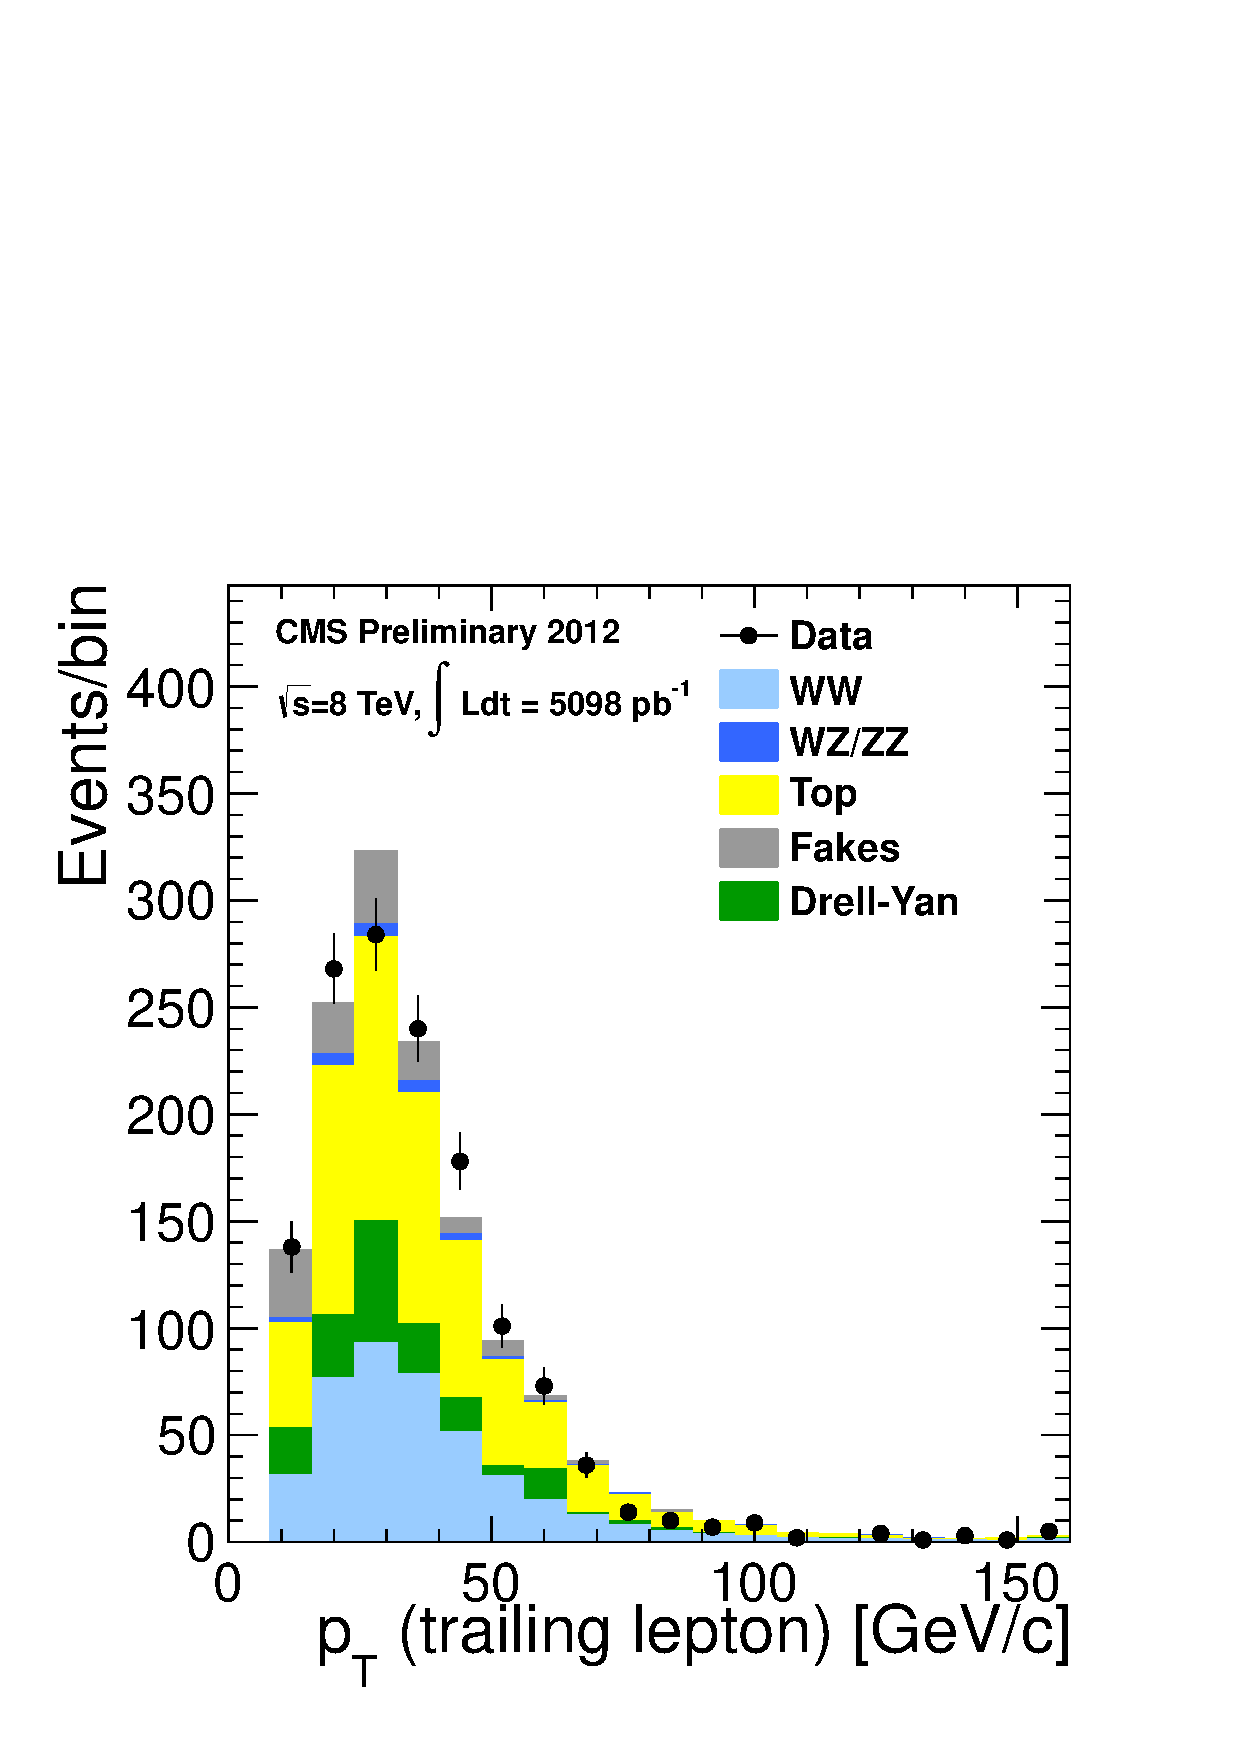
\includegraphics[width=.3\textwidth]{figures/hww_analysis16_0_ALL_incl_1j_pt2.pdf}
}
\subfigure[]{
\centering
\label{subfig:ww_ptmin_2j}
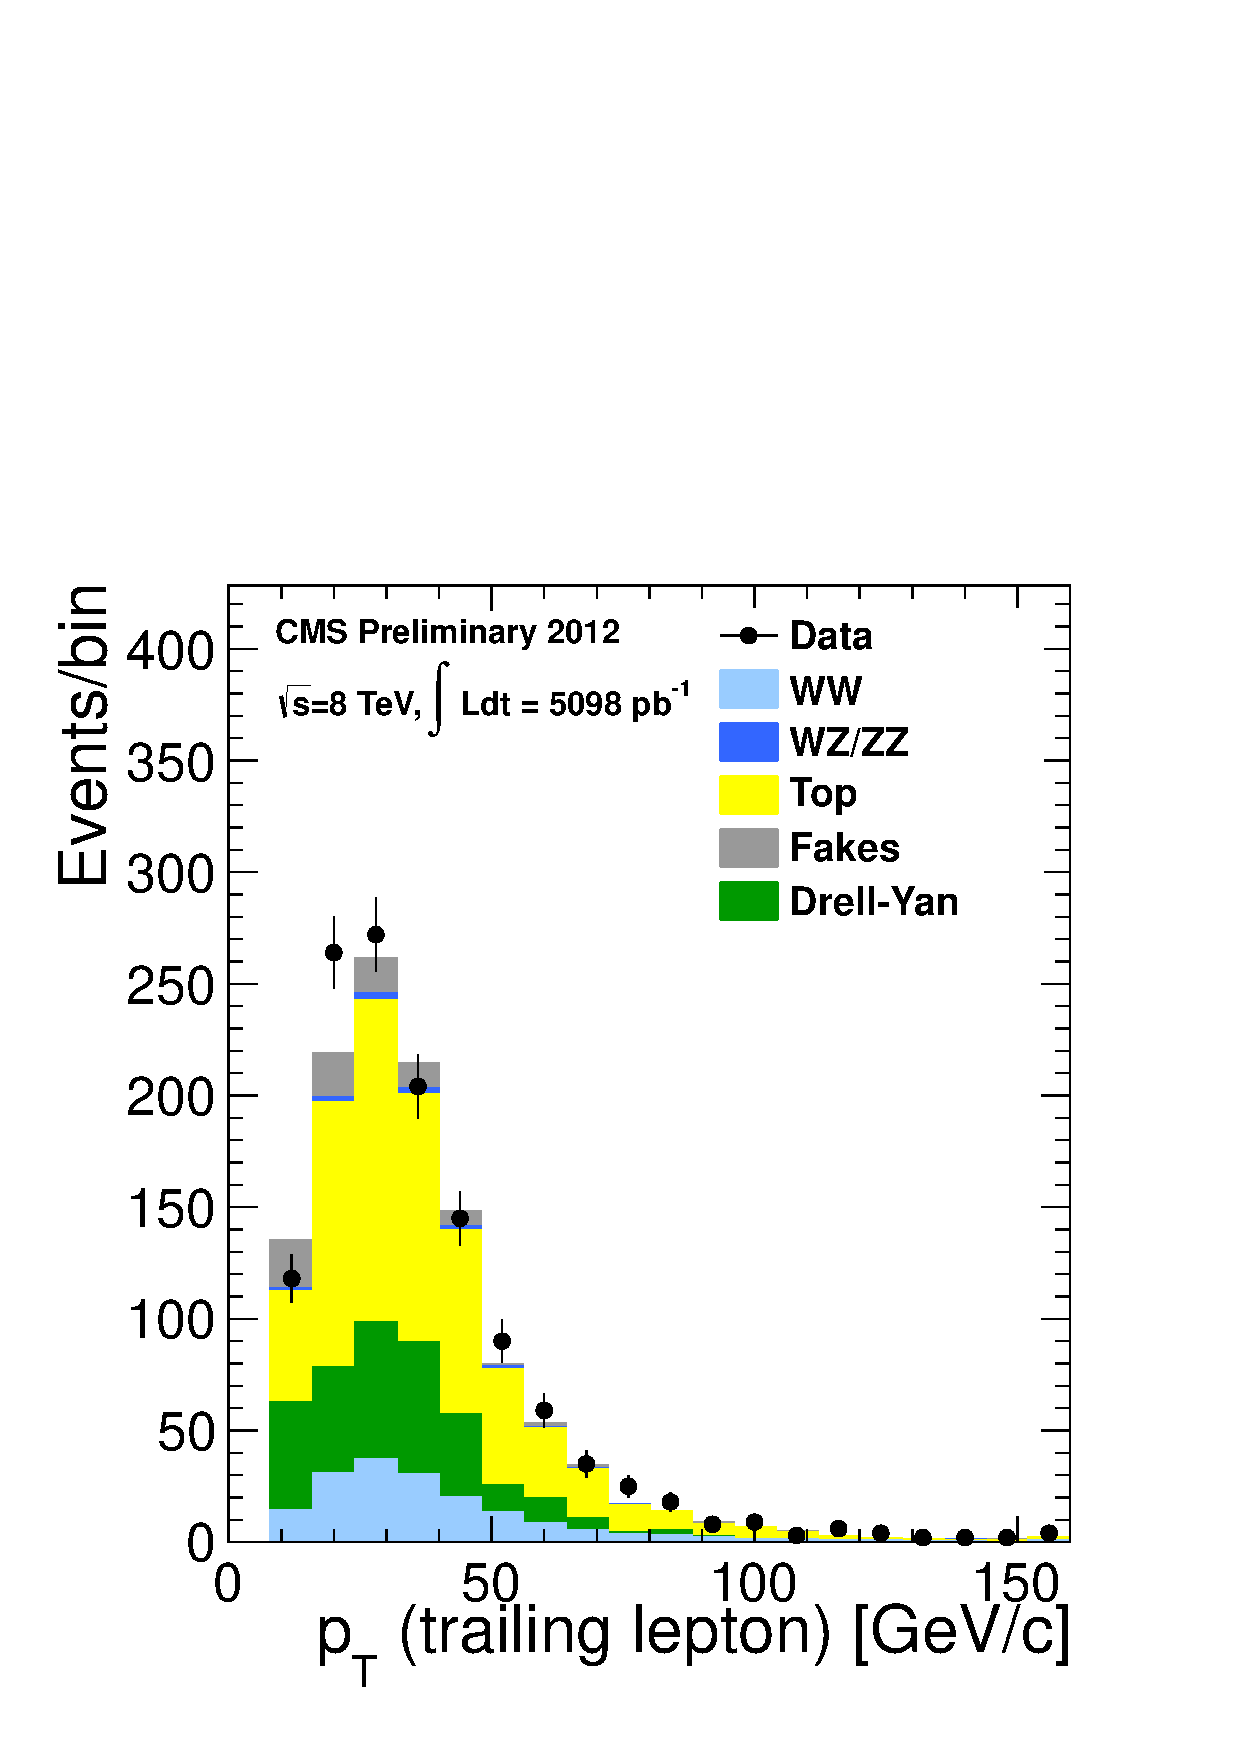
\includegraphics[width=.3\textwidth]{figures/hww_analysis16_0_ALL_incl_2j_pt2.pdf}
}
\caption{Trailing lepton $p_T$ distribution after WW selection for \intlumiEightTeV of data in the 0-jet \subref{subfig:ww_ptmin_0j}, 
1-jet \subref{subfig:ww_ptmin_1j} and 2-jet \subref{subfig:ww_ptmin_2j} bin analyses. 
MC is scaled to data-driven estimates for all processes.}
\label{fig:ww_ptmin}
\end{figure}

\begin{figure}[!hbtp]
\centering
\subfigure[]{
\centering
\label{subfig:ww_ptmax_0j}
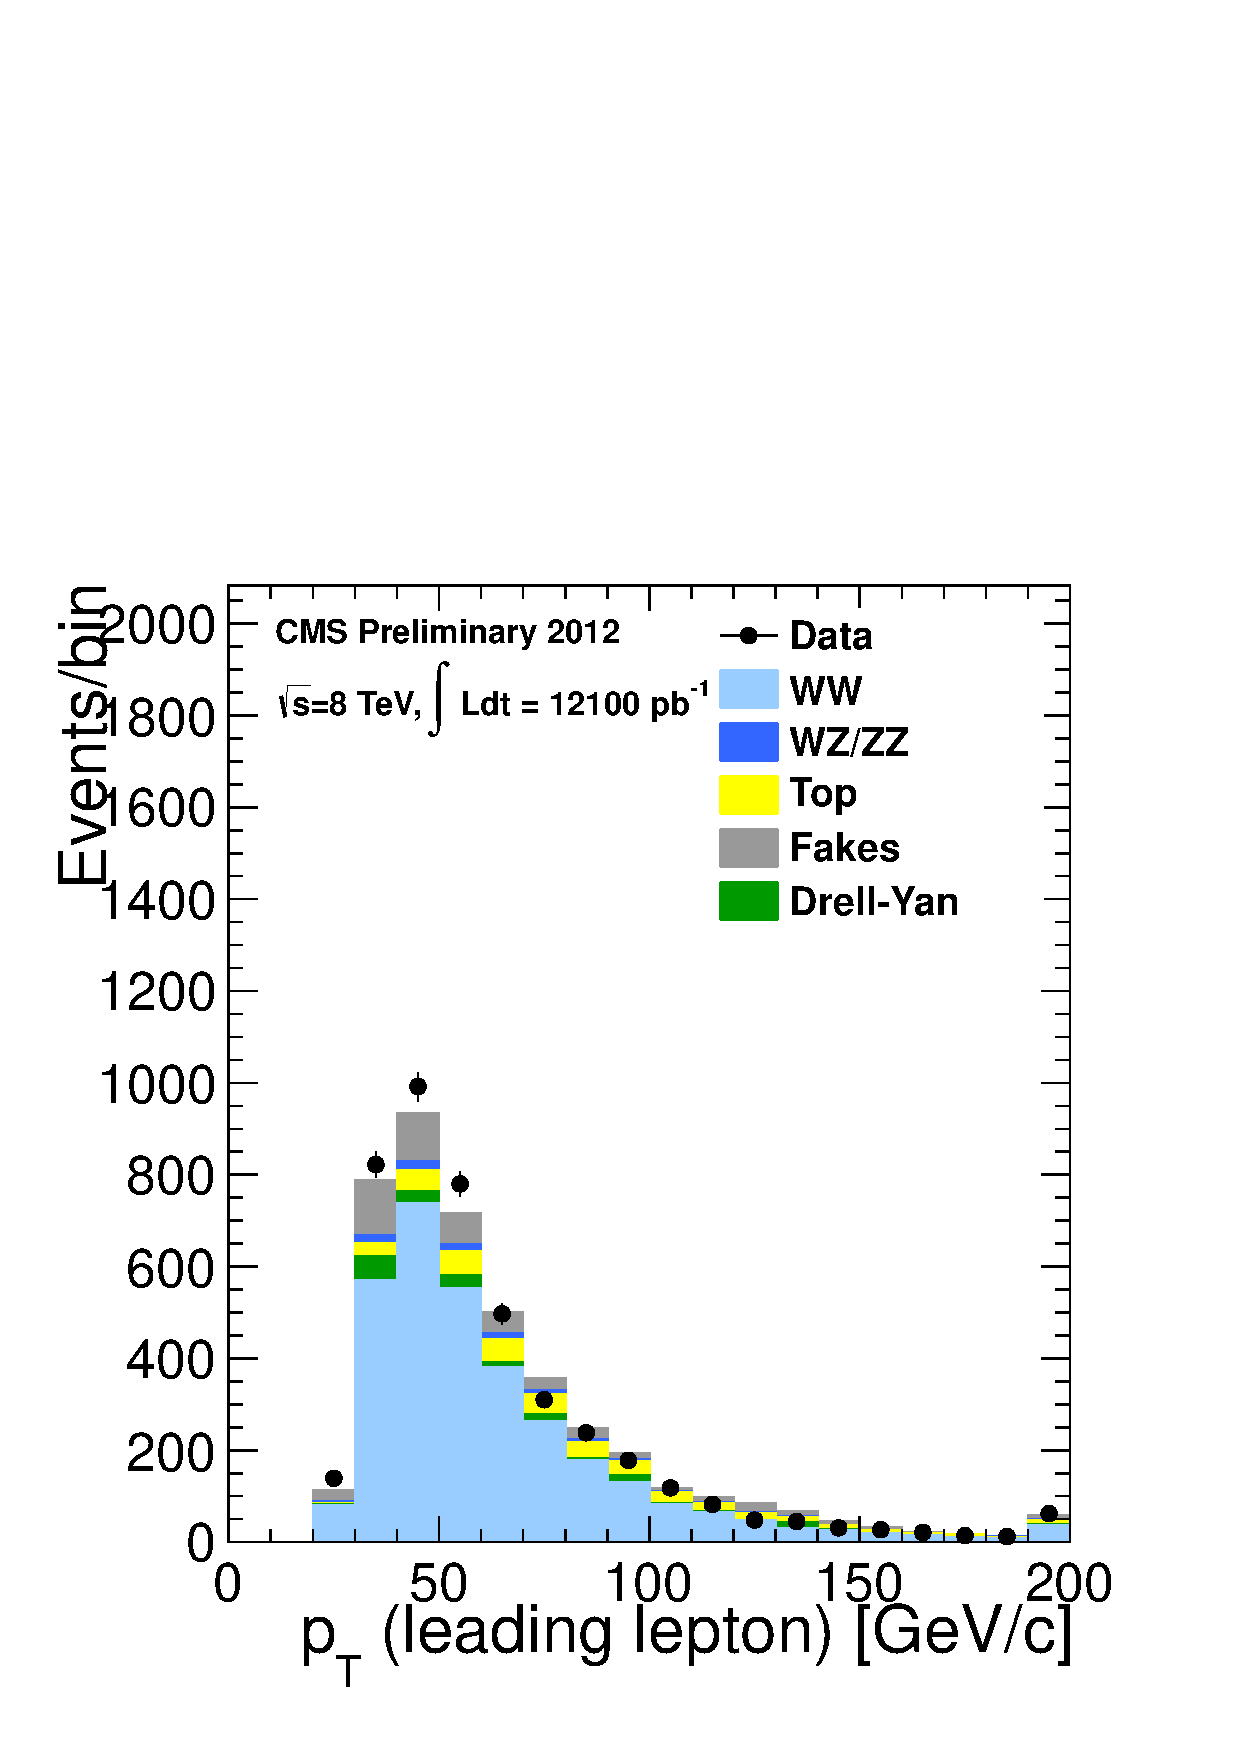
\includegraphics[width=.3\textwidth]{figures/hww_analysis16_0_ALL_incl_0j_pt1.pdf}
}
\subfigure[]{
\centering
\label{subfig:ww_ptmax_1j}
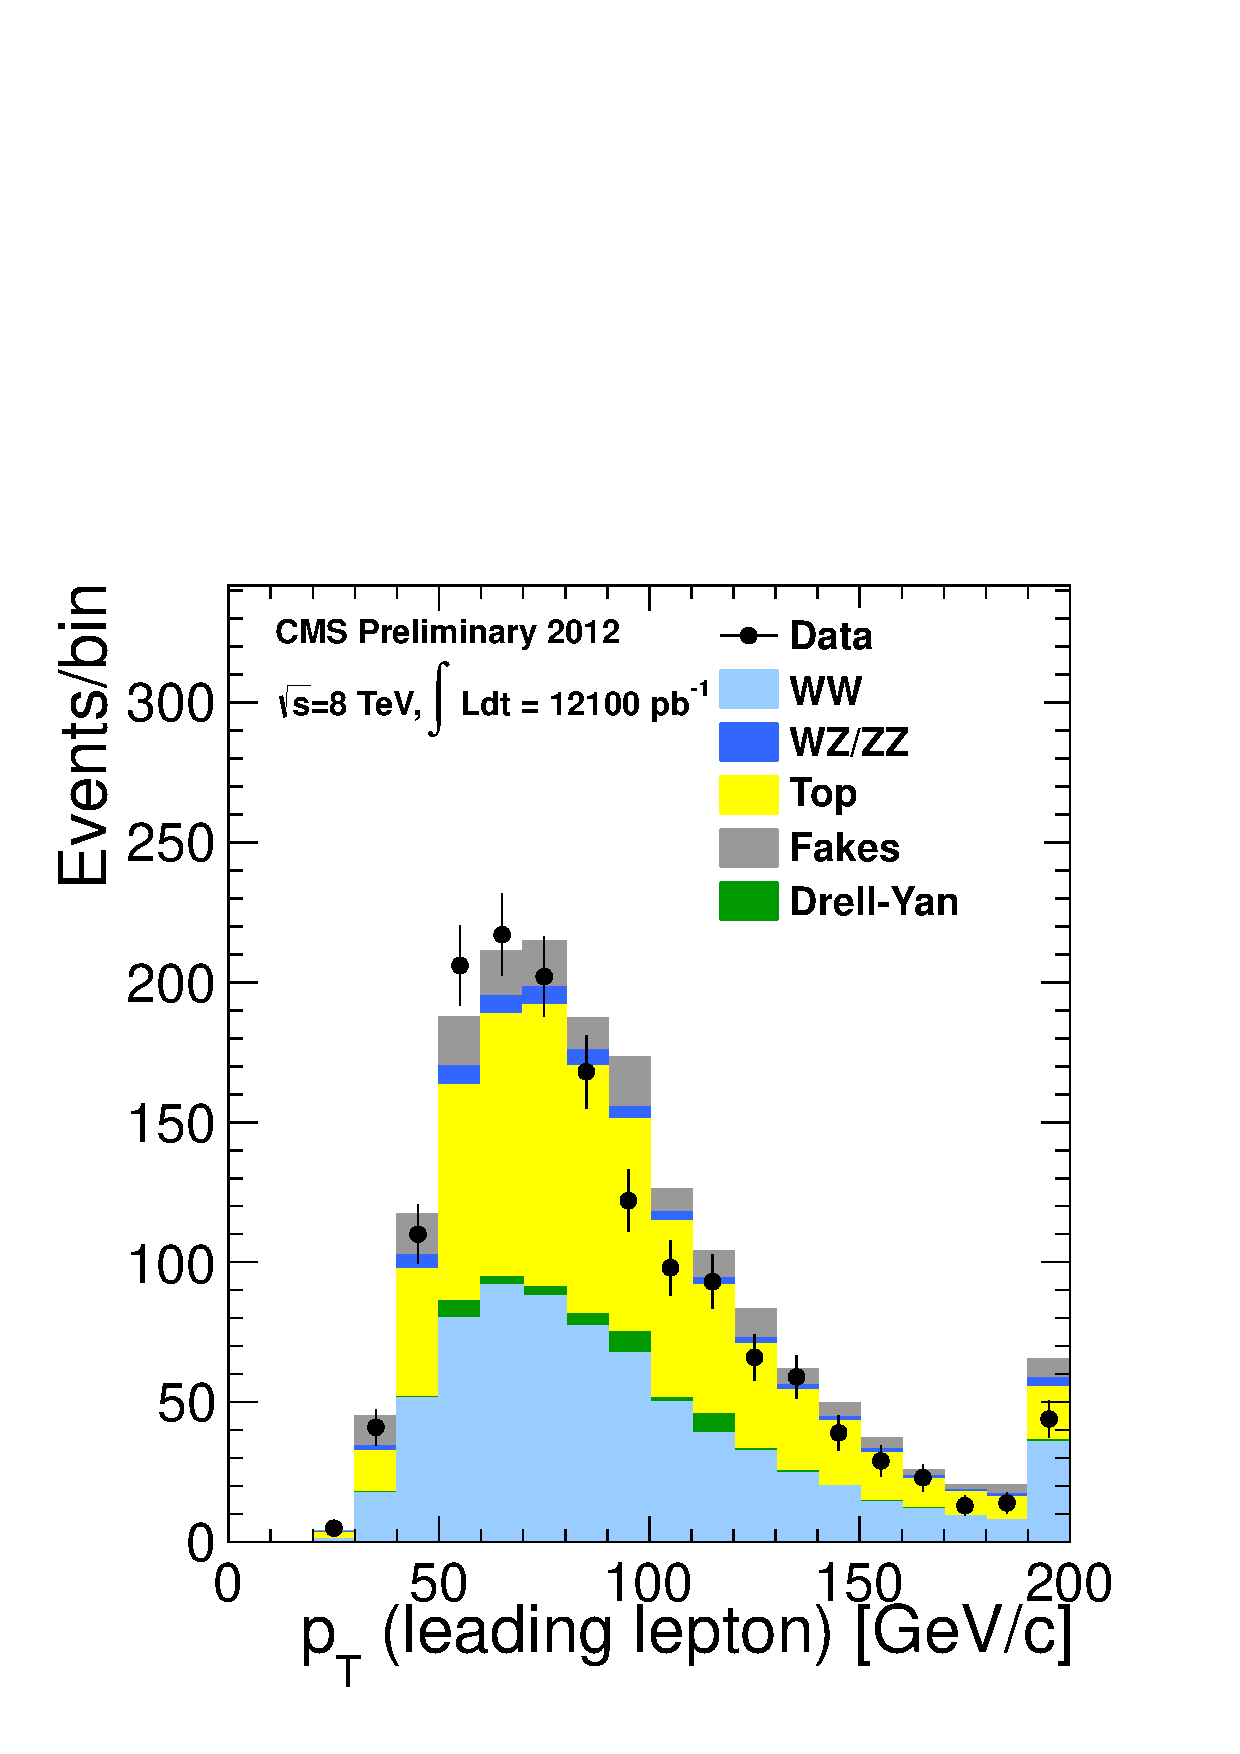
\includegraphics[width=.3\textwidth]{figures/hww_analysis16_0_ALL_incl_1j_pt1.pdf}
}
\subfigure[]{
\centering
\label{subfig:ww_ptmax_2j}
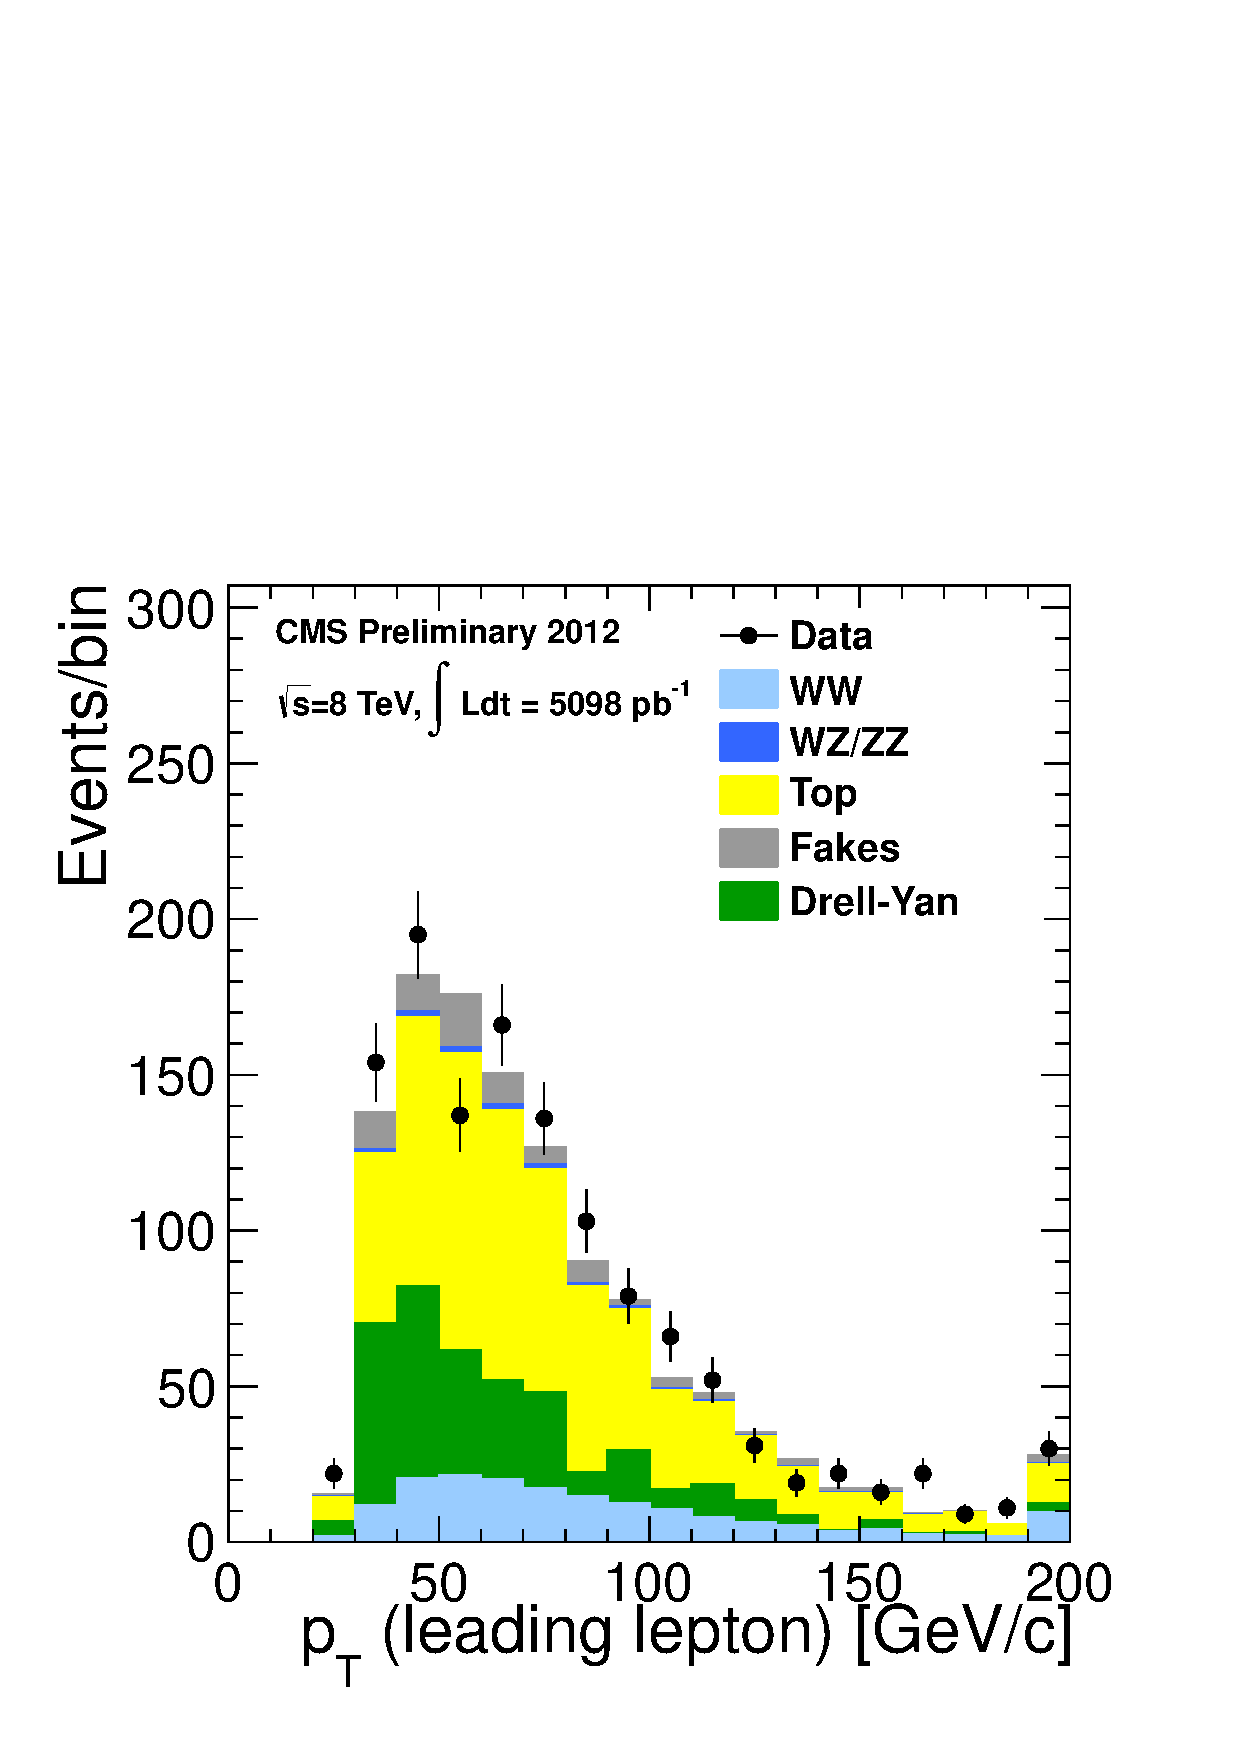
\includegraphics[width=.3\textwidth]{figures/hww_analysis16_0_ALL_incl_2j_pt1.pdf}
}\\
\caption{Leading lepton $p_T$ distribution after WW selection for \intlumiEightTeV of data in the 0-jet \subref{subfig:ww_ptmax_0j}, 
1-jet \subref{subfig:ww_ptmax_1j} and 2-jet \subref{subfig:ww_ptmax_2j} bin analyses. 
MC is scaled to data-driven estimates for all processes.}
\label{fig:ww_ptmax}
\end{figure}

\begin{figure}[!hbtp]
\centering
\subfigure[]{
\centering
\label{subfig:ww_pmet_0j}
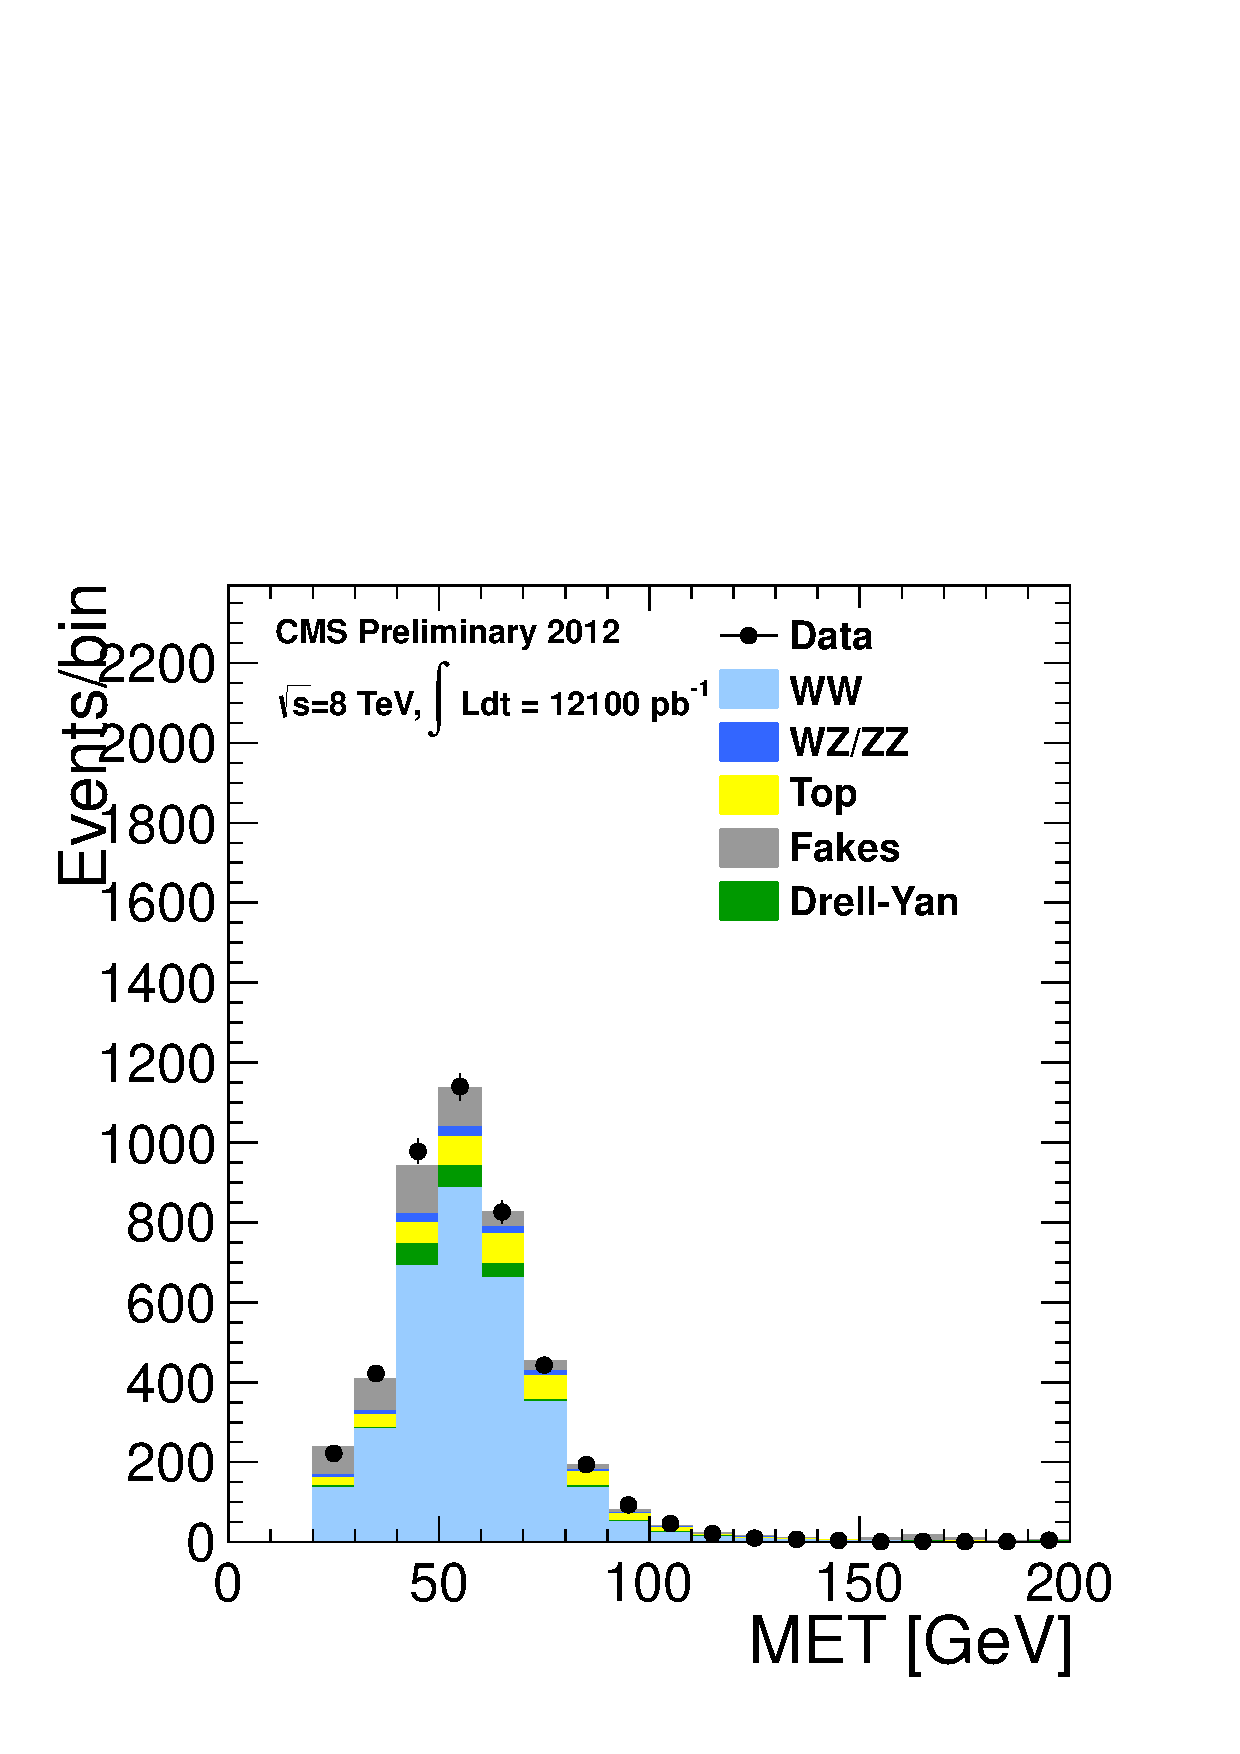
\includegraphics[width=.3\textwidth]{figures/hww_analysis16_0_ALL_incl_0j_met.pdf}
}
\subfigure[]{
\centering
\label{subfig:ww_pmet_1j}
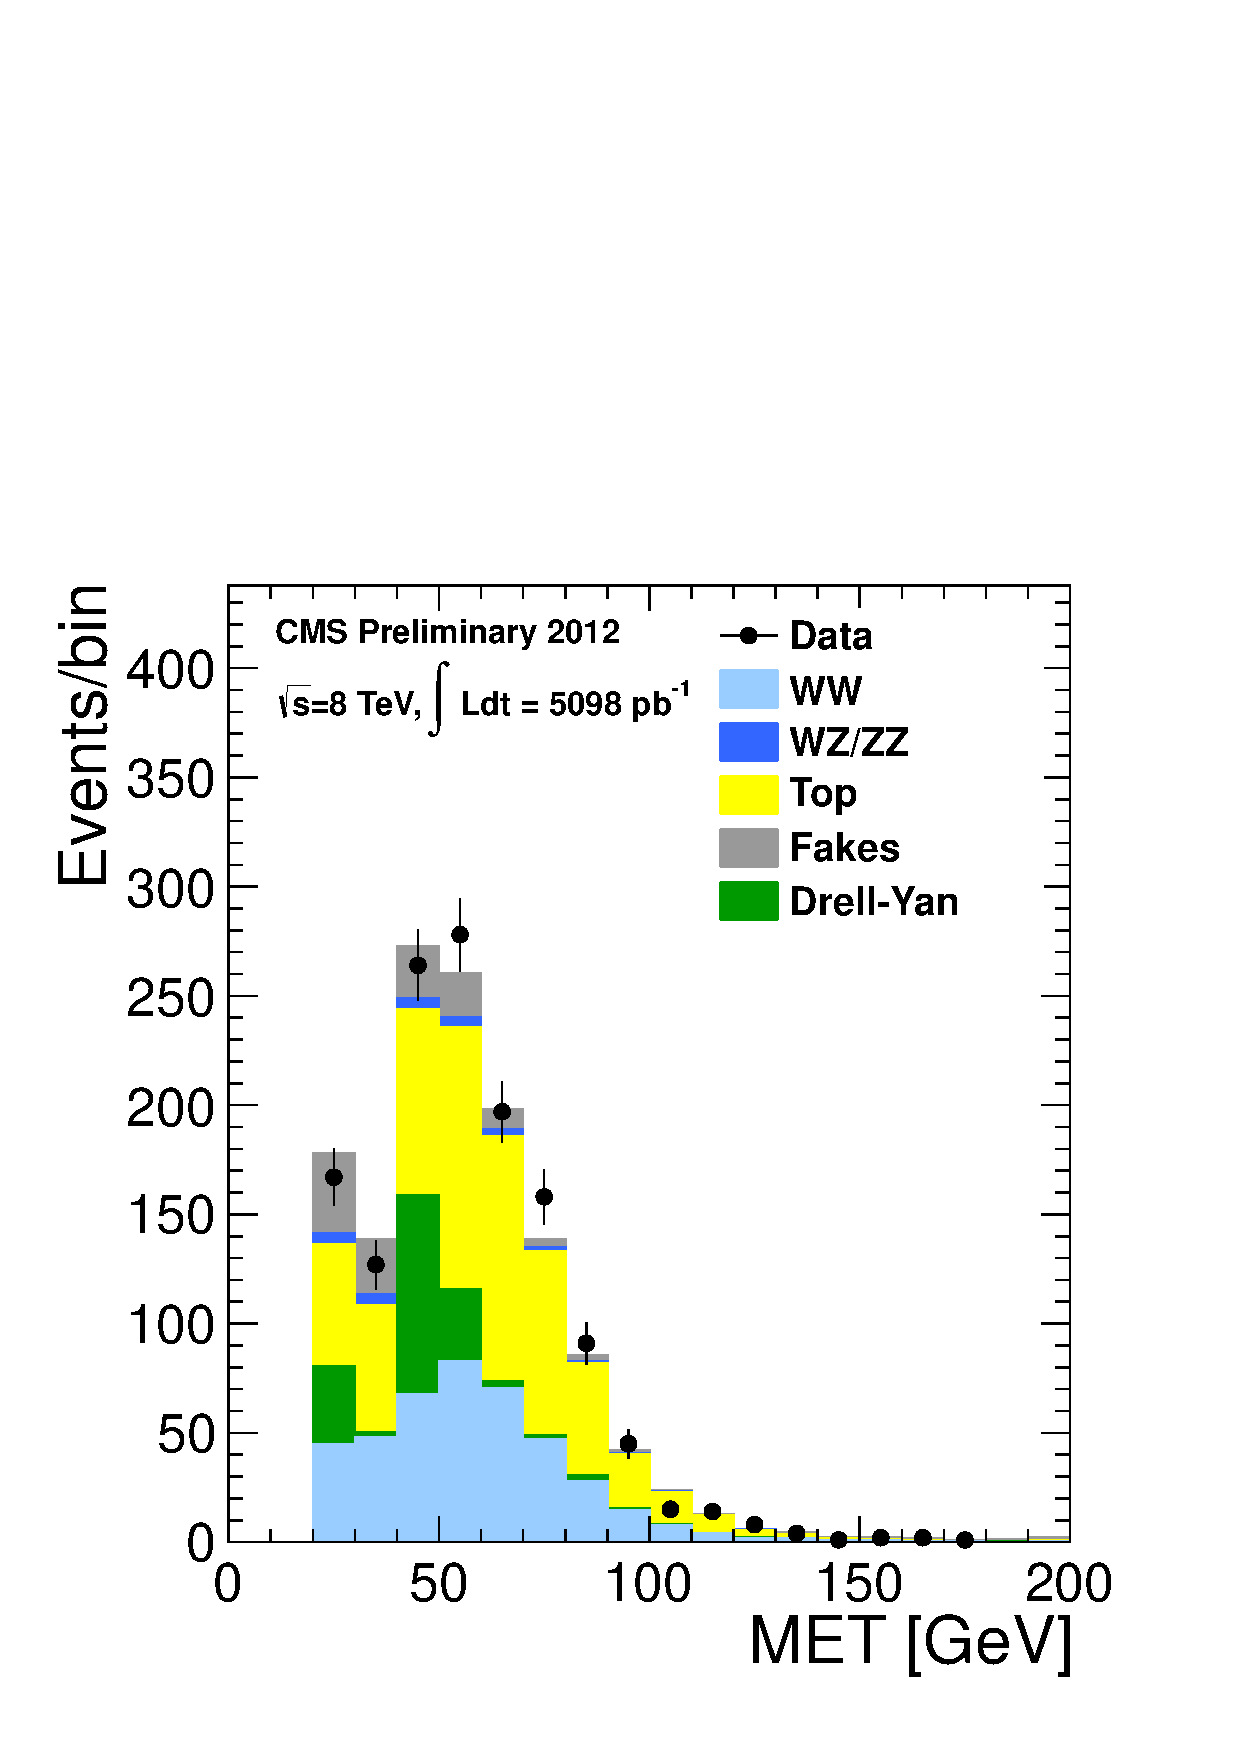
\includegraphics[width=.3\textwidth]{figures/hww_analysis16_0_ALL_incl_1j_met.pdf}
}
\subfigure[]{
\centering
\label{subfig:ww_pmet_2j}
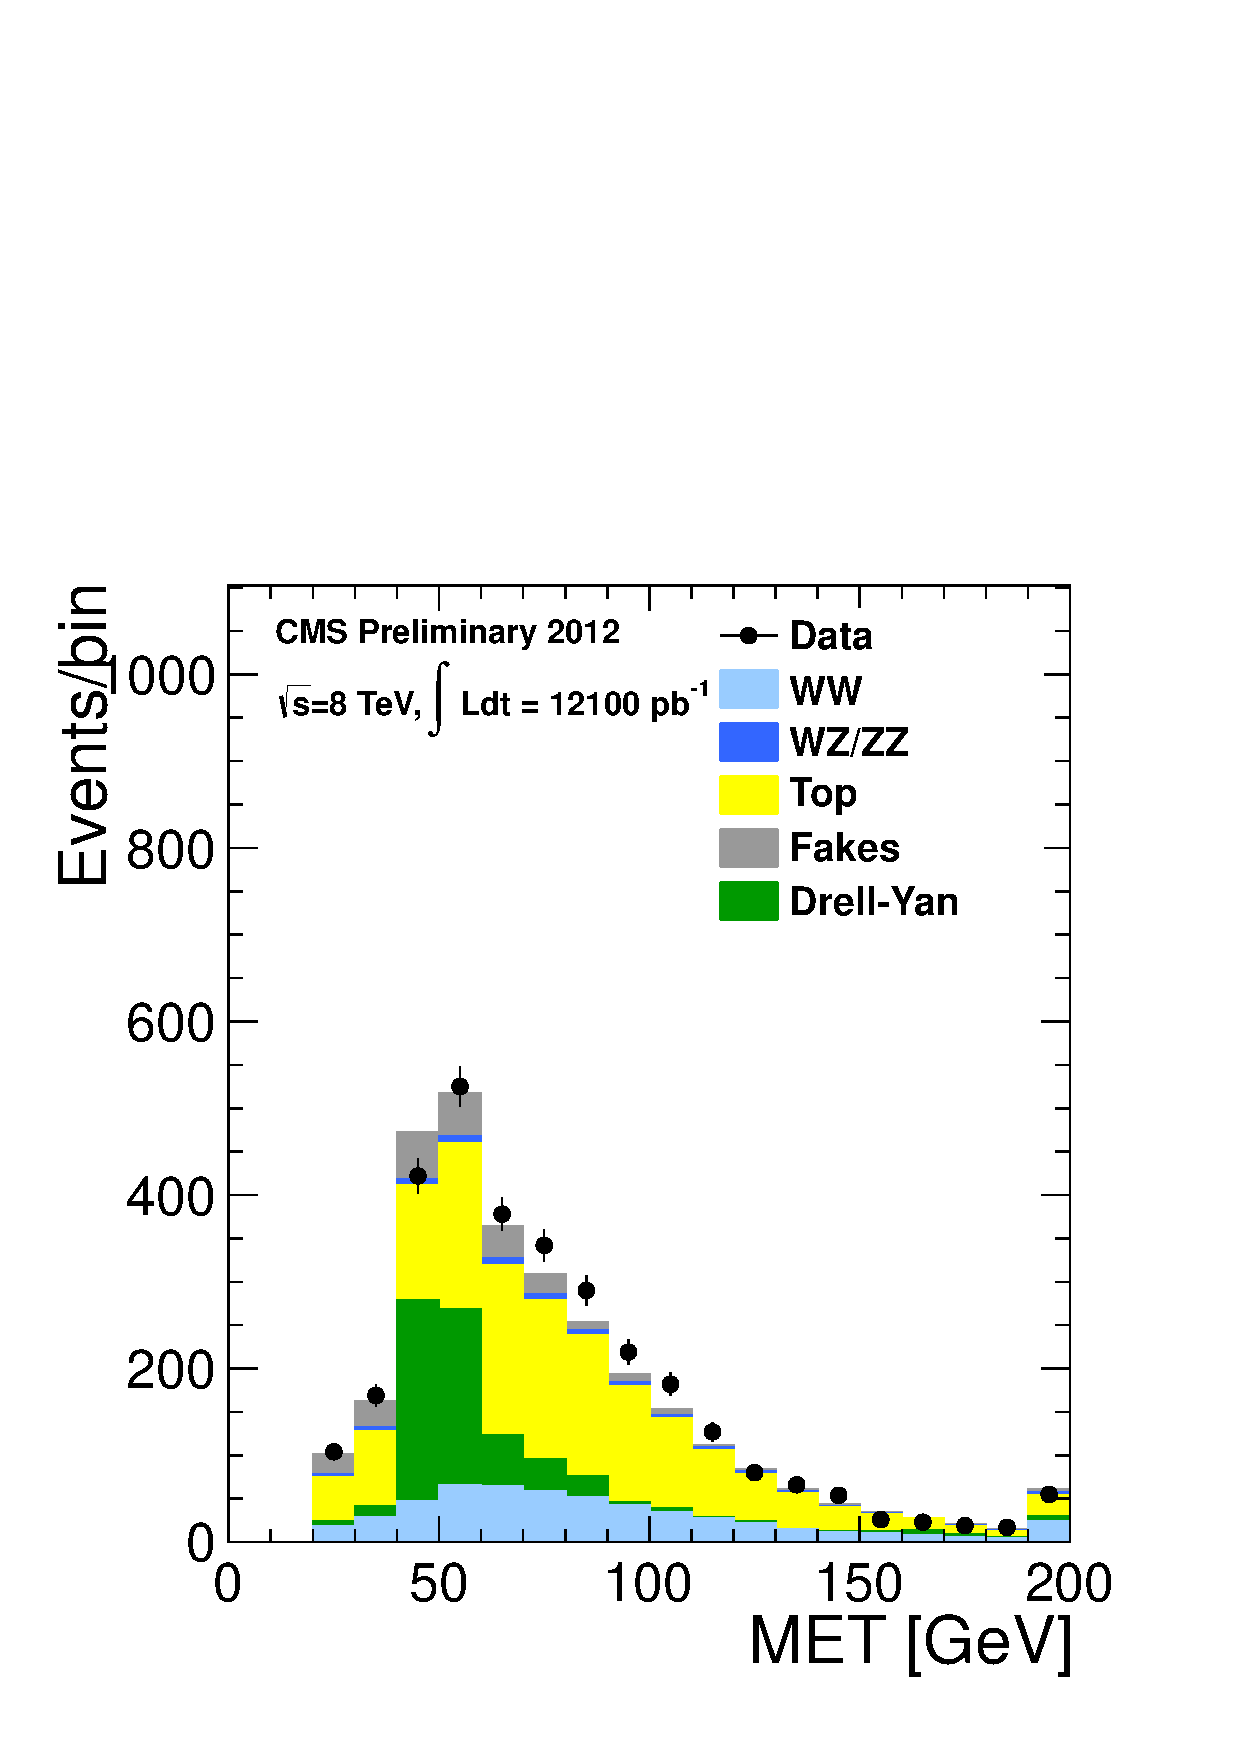
\includegraphics[width=.3\textwidth]{figures/hww_analysis16_0_ALL_incl_2j_met.pdf}
}\\
\caption{The $\met$ distributions distribution after WW selection for \intlumiEightTeV of data in the 0-jet \subref{subfig:ww_pmet_0j}, 
1-jet \subref{subfig:ww_pmet_1j} and 2-jet \subref{subfig:ww_pmet_2j} bin analyses. 
Note that for the 0 and 1 Jet bins, $min(\text{proj}_\text{trk-MET}, \text{proj}_\text{PFMET})$ are plotted, 
while for the 2-jet bin, PFMET is used. MC is scaled to data-driven estimates for all processes.}
\label{fig:ww_pmet}
\end{figure}

\begin{figure}[!hbtp]
\centering
\subfigure[]{
\centering
\label{subfig:ww_mt_0j}
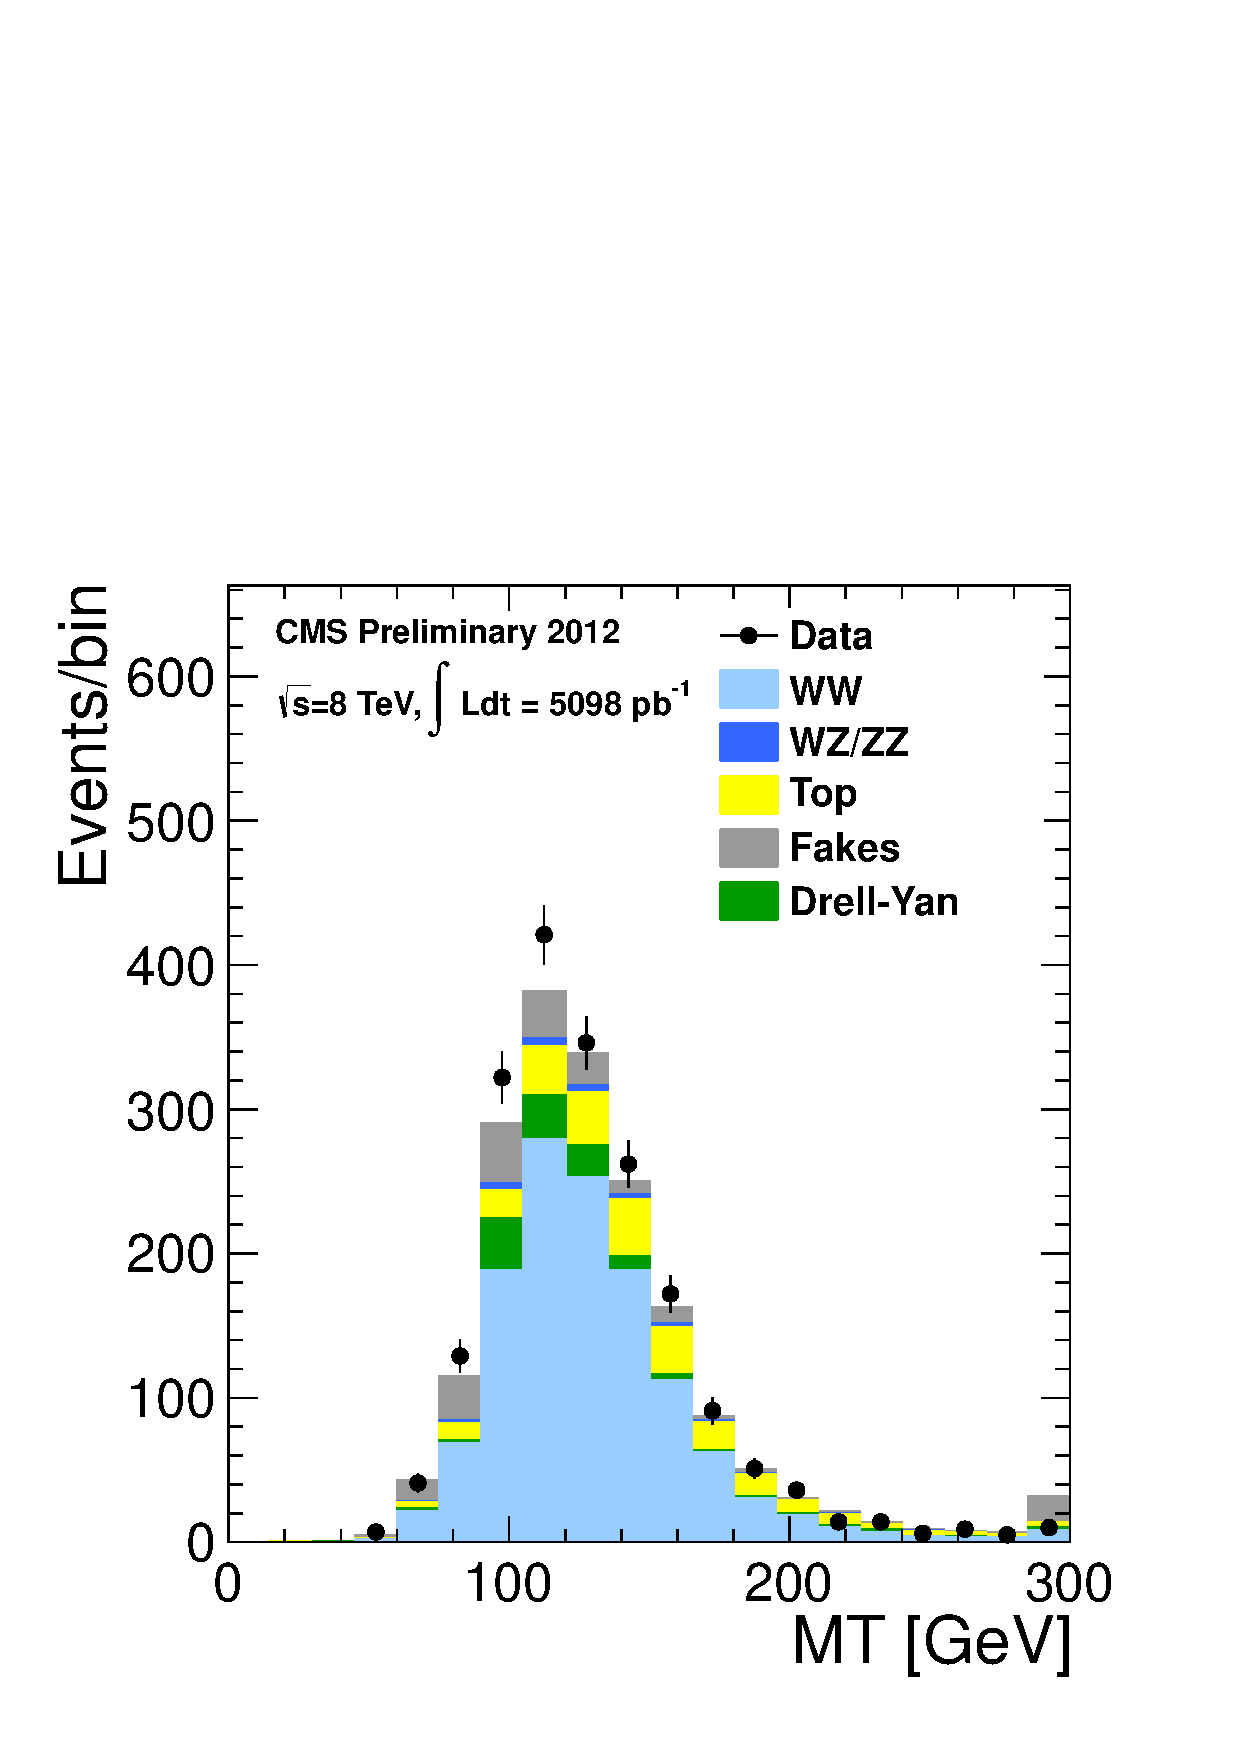
\includegraphics[width=.3\textwidth]{figures/hww_analysis16_0_ALL_incl_0j_mt.pdf}
}
\subfigure[]{
\centering
\label{subfig:ww_mt_1j}
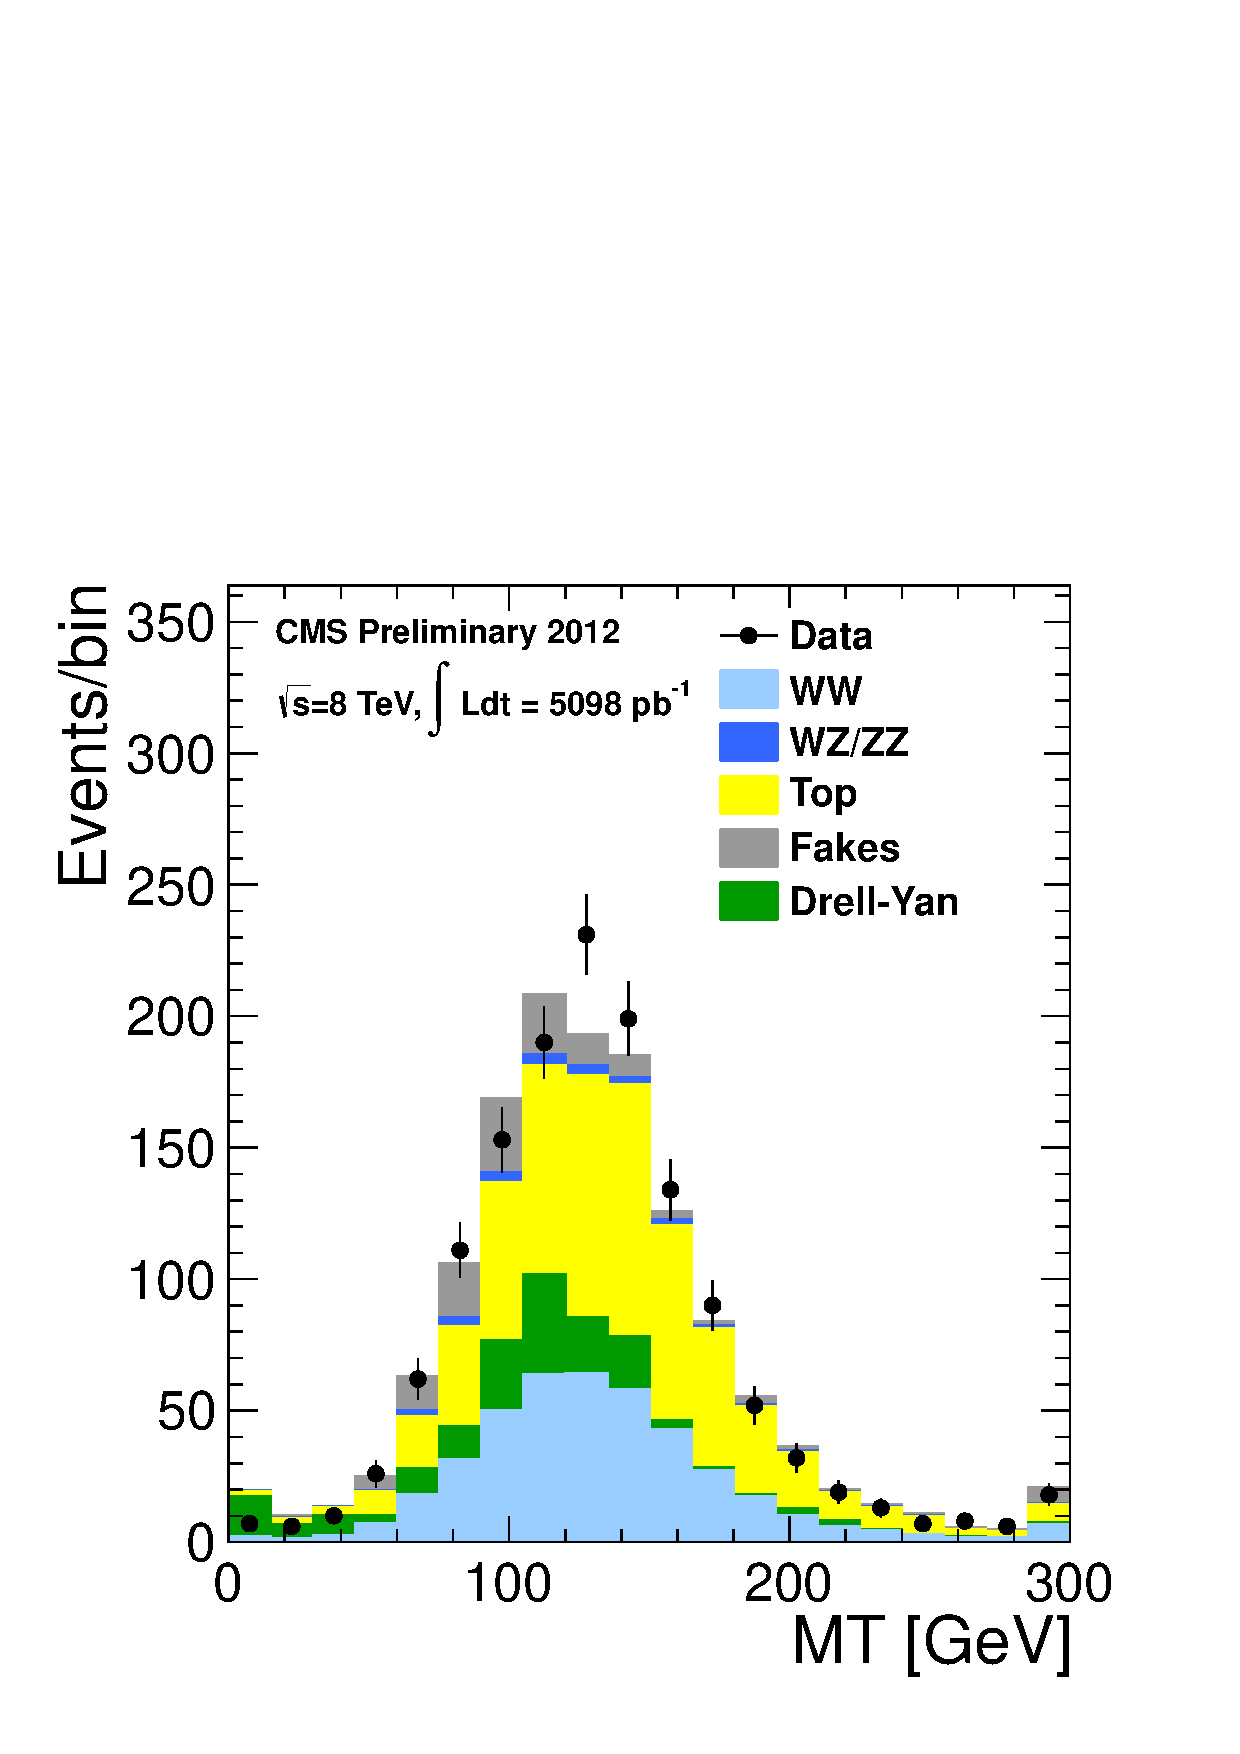
\includegraphics[width=.3\textwidth]{figures/hww_analysis16_0_ALL_incl_1j_mt.pdf}
}
\subfigure[]{
\centering
\label{subfig:ww_mt_2j}
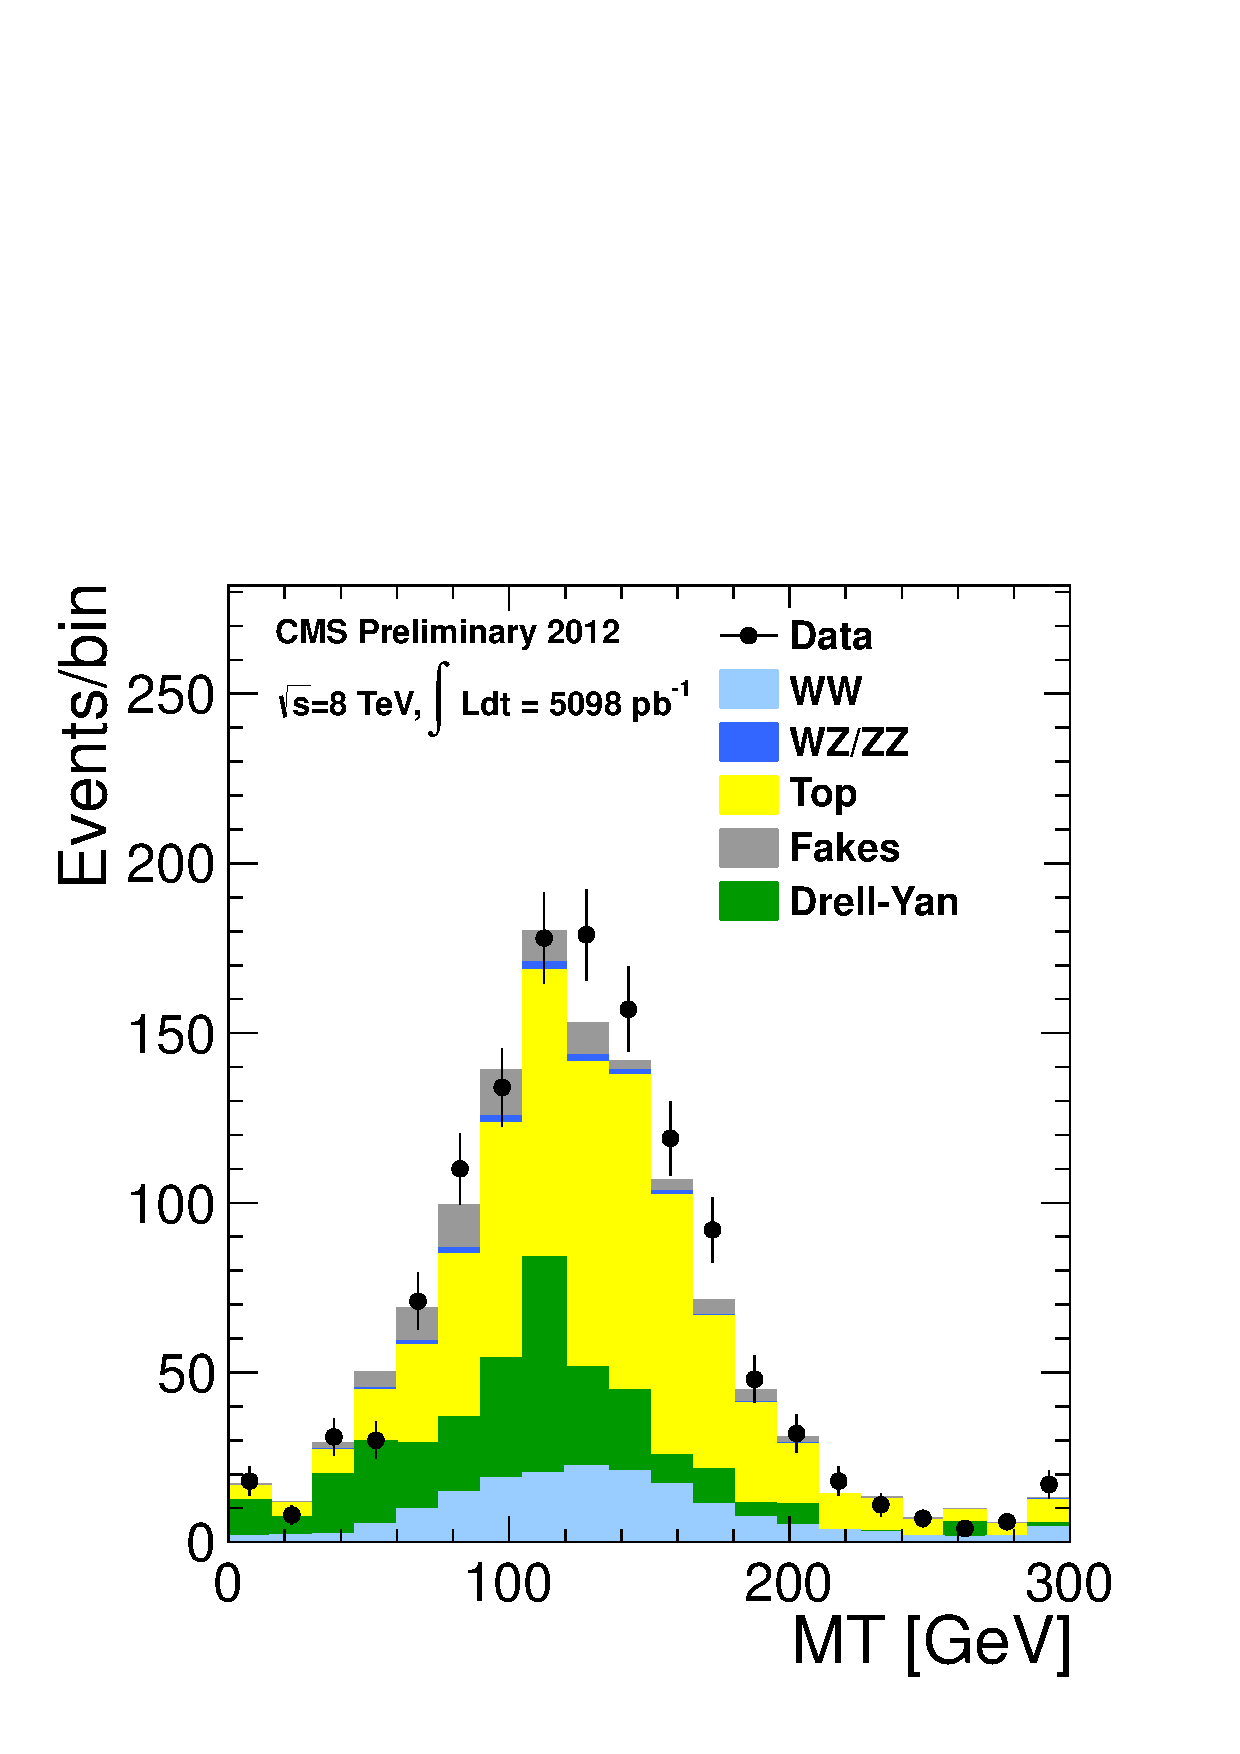
\includegraphics[width=.3\textwidth]{figures/hww_analysis16_0_ALL_incl_2j_mt.pdf}
} \\
\caption{Transverse mass distribution after WW selection for \intlumiEightTeV of data in the 0-jet \subref{subfig:ww_mt_0j}, 
1-jet \subref{subfig:ww_mt_1j} and 2-jet \subref{subfig:ww_mt_2j} bin analyses. 
MC is scaled to data-driven estimates for all processes.}
\label{fig:ww_mt}
\end{figure}

\begin{figure}[!hbtp]
\centering
\subfigure[]{
\centering
\label{subfig:ww_dilmass_0j}
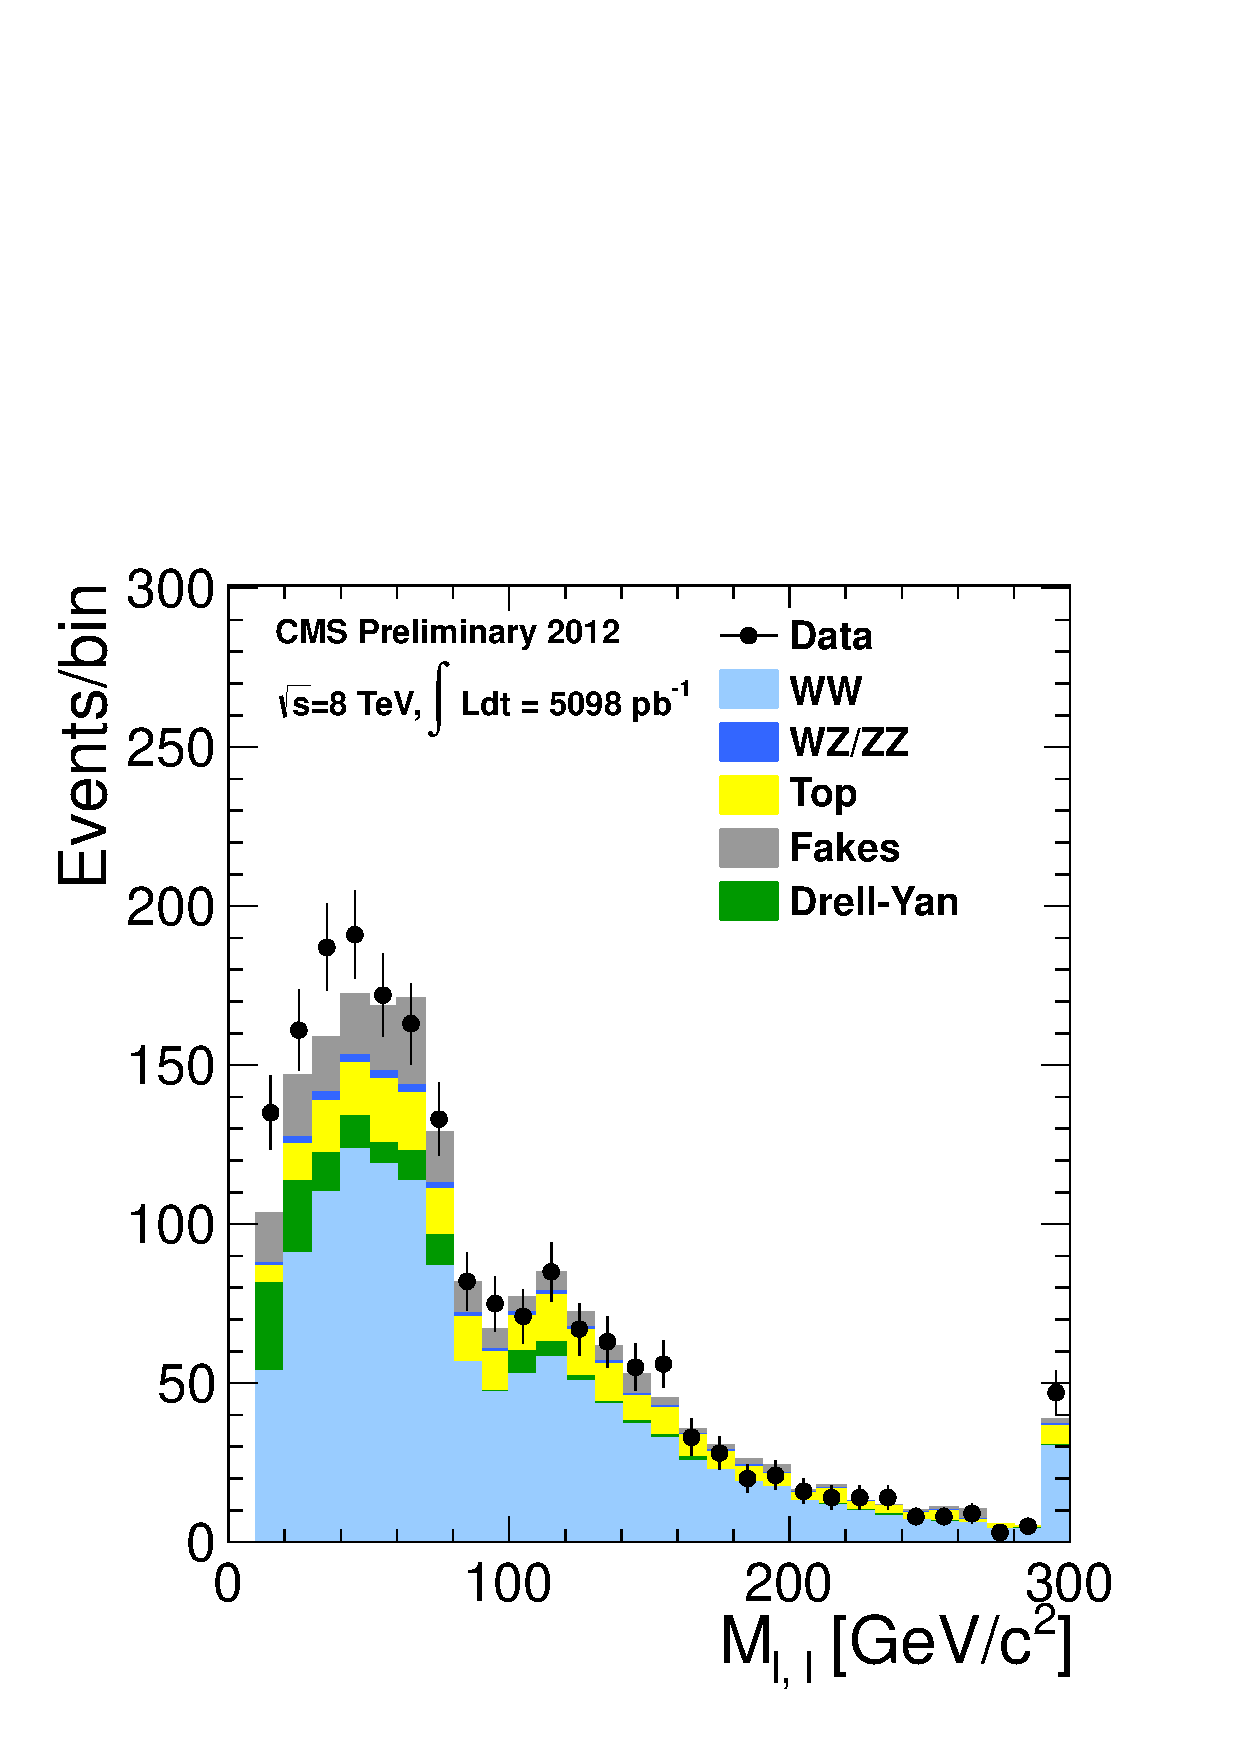
\includegraphics[width=.3\textwidth]{figures/hww_analysis16_0_ALL_incl_0j_mll.pdf}
}
\subfigure[]{
\centering
\label{subfig:ww_dilmass_1j}
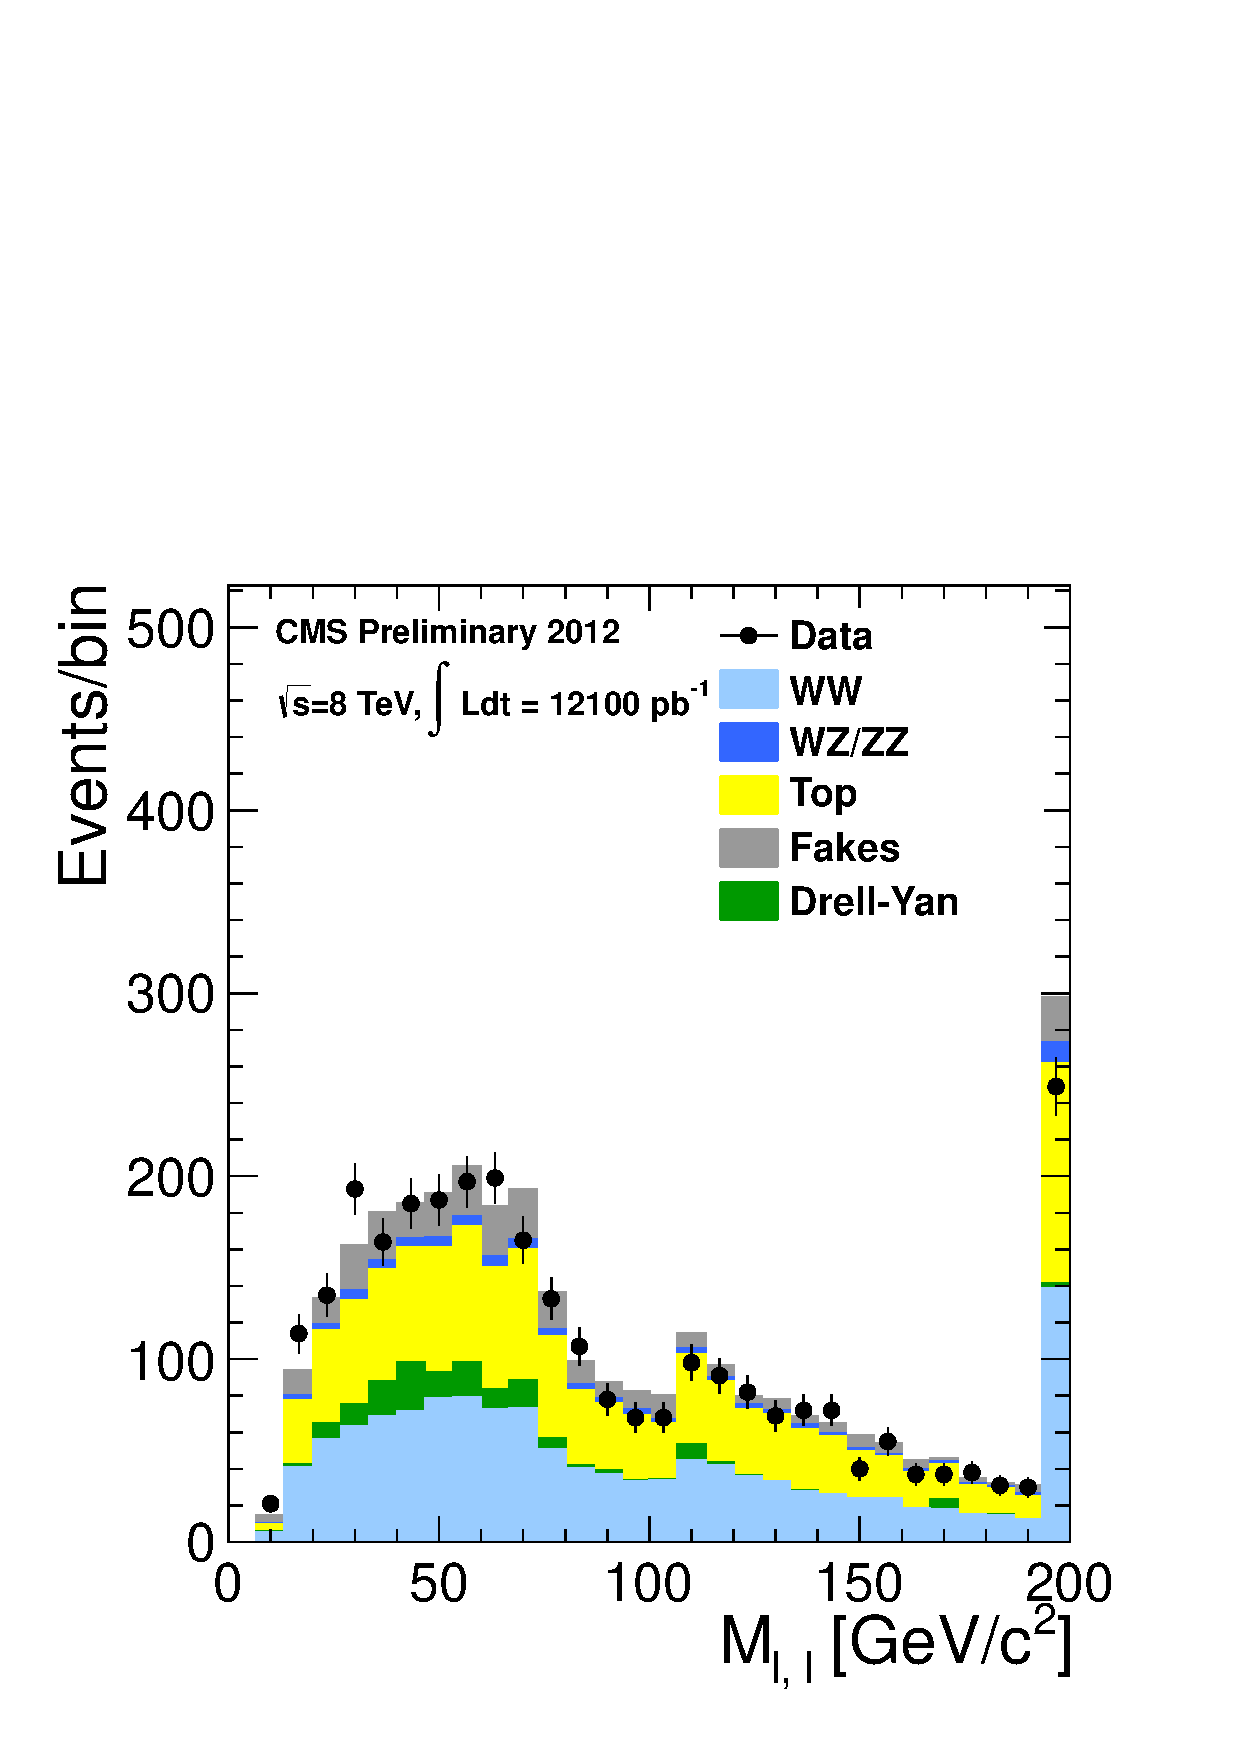
\includegraphics[width=.3\textwidth]{figures/hww_analysis16_0_ALL_incl_1j_mll.pdf}
}
\subfigure[]{
\centering
\label{subfig:ww_dilmass_2j}
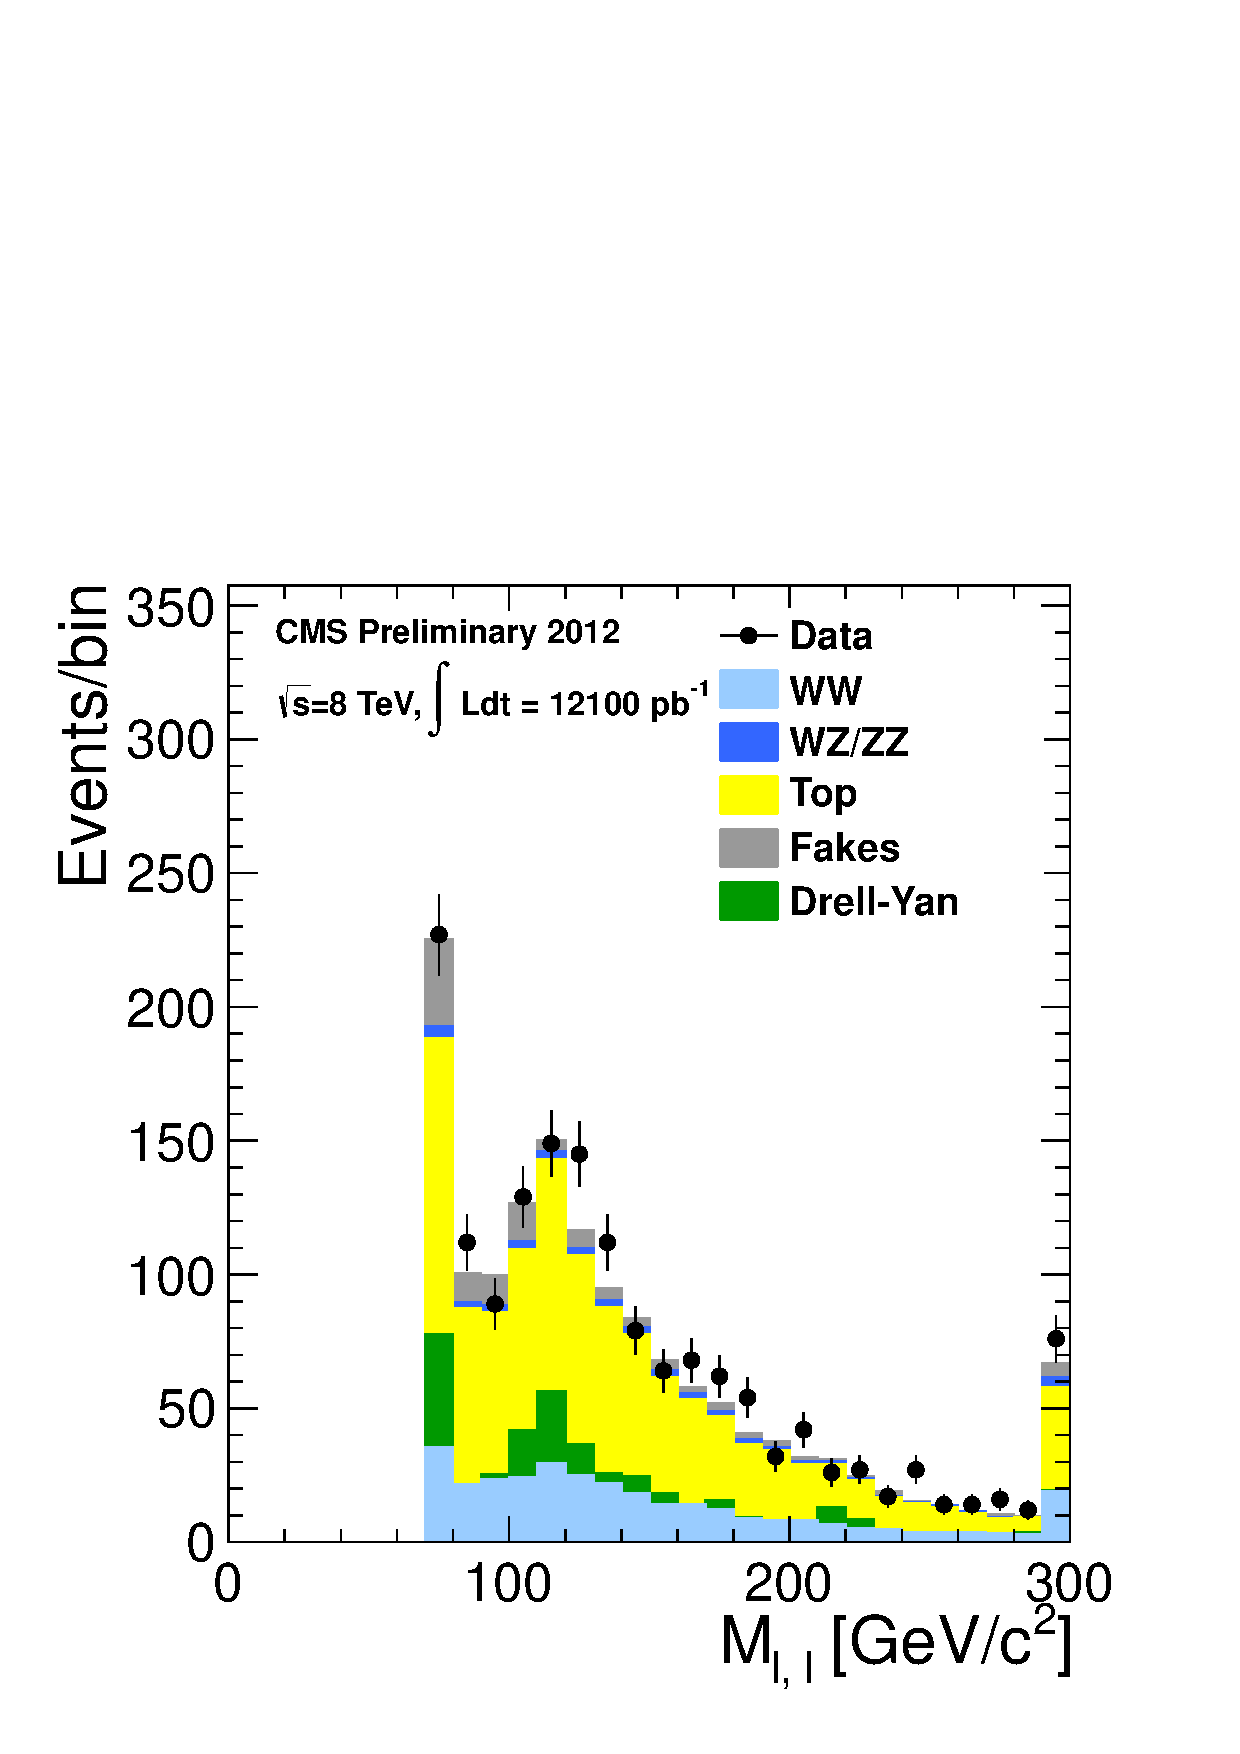
\includegraphics[width=.3\textwidth]{figures/hww_analysis16_0_ALL_incl_2j_mll.pdf}
} \\
\caption{Invariant dilepton mass distribution after WW selection for \intlumiEightTeV of data in the 0-jet \subref{subfig:ww_dilmass_0j}, 
1-jet \subref{subfig:ww_dilmass_1j} and 2-jet \subref{subfig:ww_dilmass_2j} bin analyses. 
MC is scaled to data-driven estimates for all processes.}
\label{fig:ww_dilmass}
\end{figure}

\begin{figure}[!hbtp]
\centering
\subfigure[]{
\centering
\label{subfig:ww_deltaphi_0j}
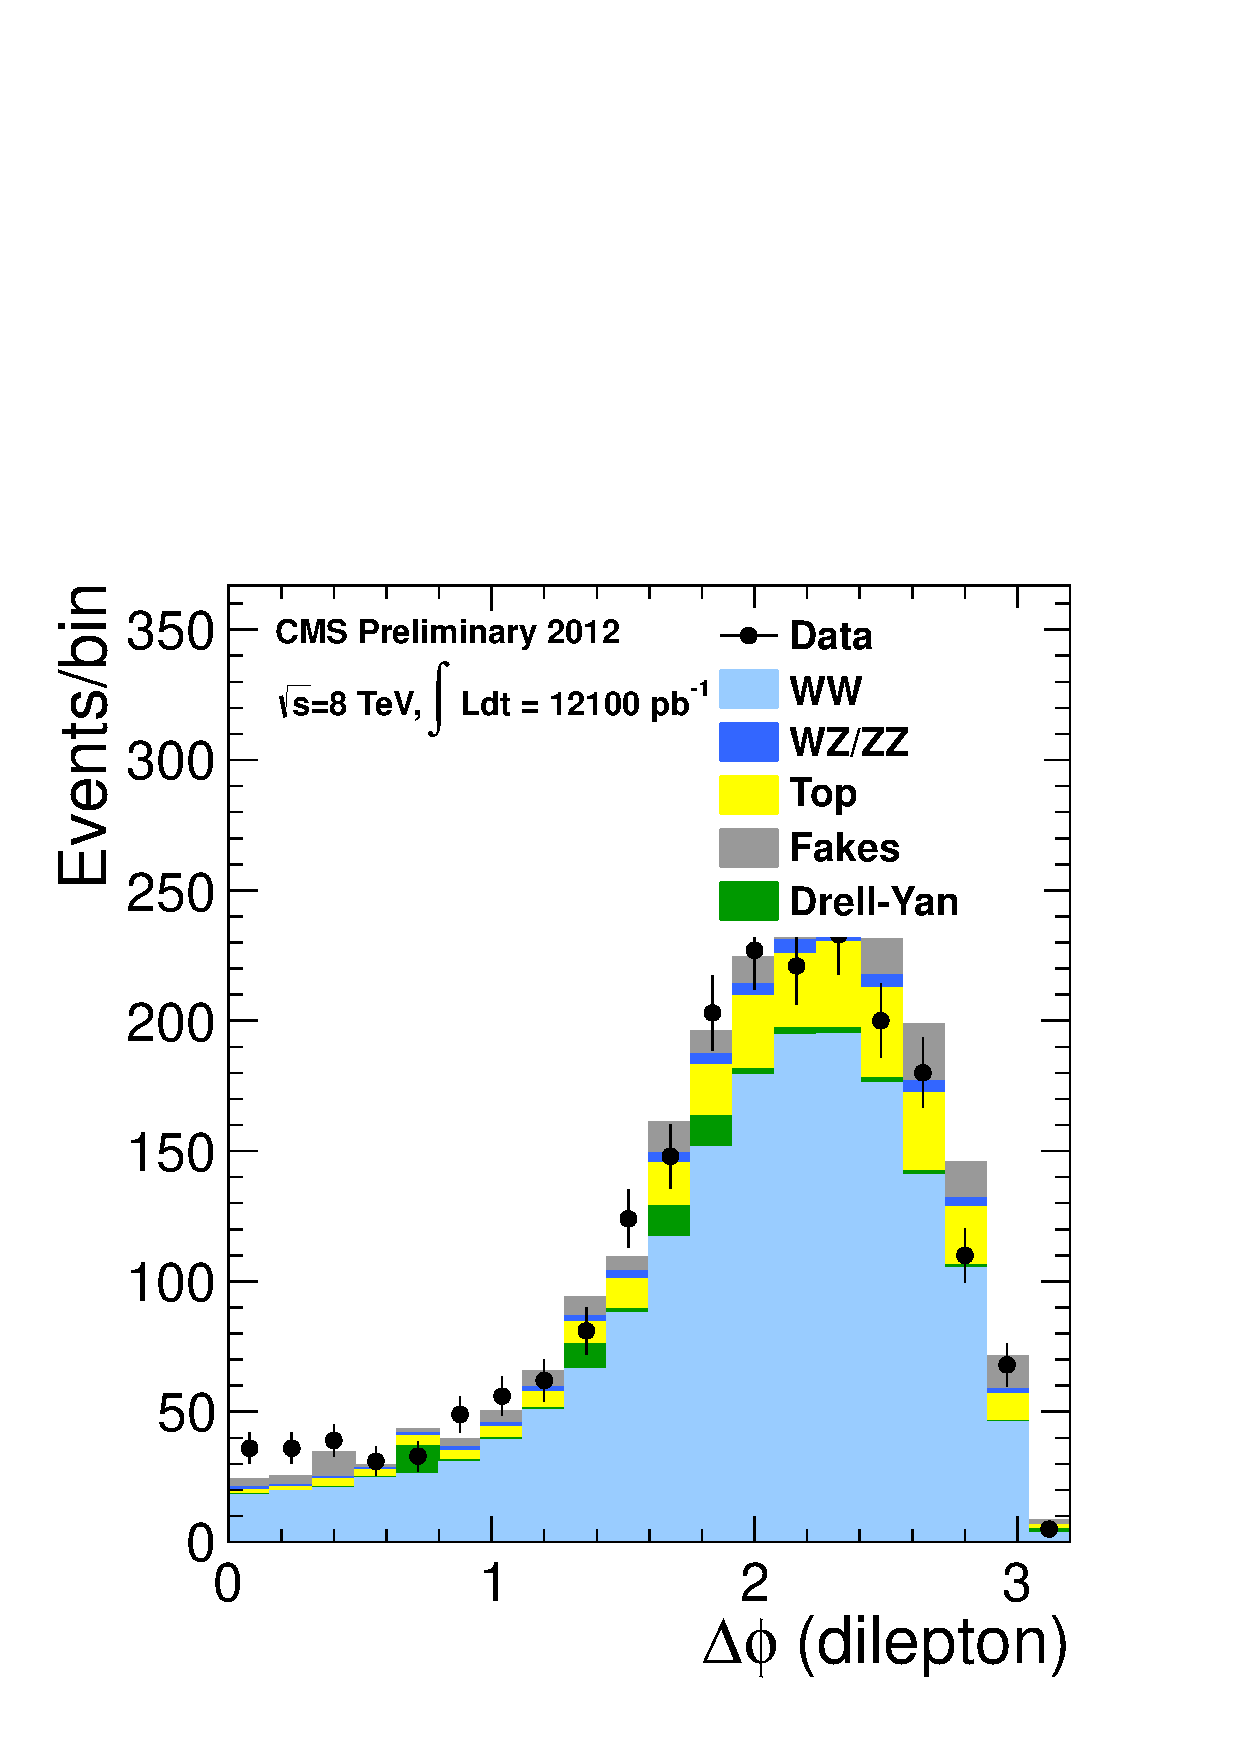
\includegraphics[width=.3\textwidth]{figures/hww_analysis16_0_ALL_incl_0j_dphi.pdf}
}
\subfigure[]{
\centering
\label{subfig:ww_deltaphi_1j}
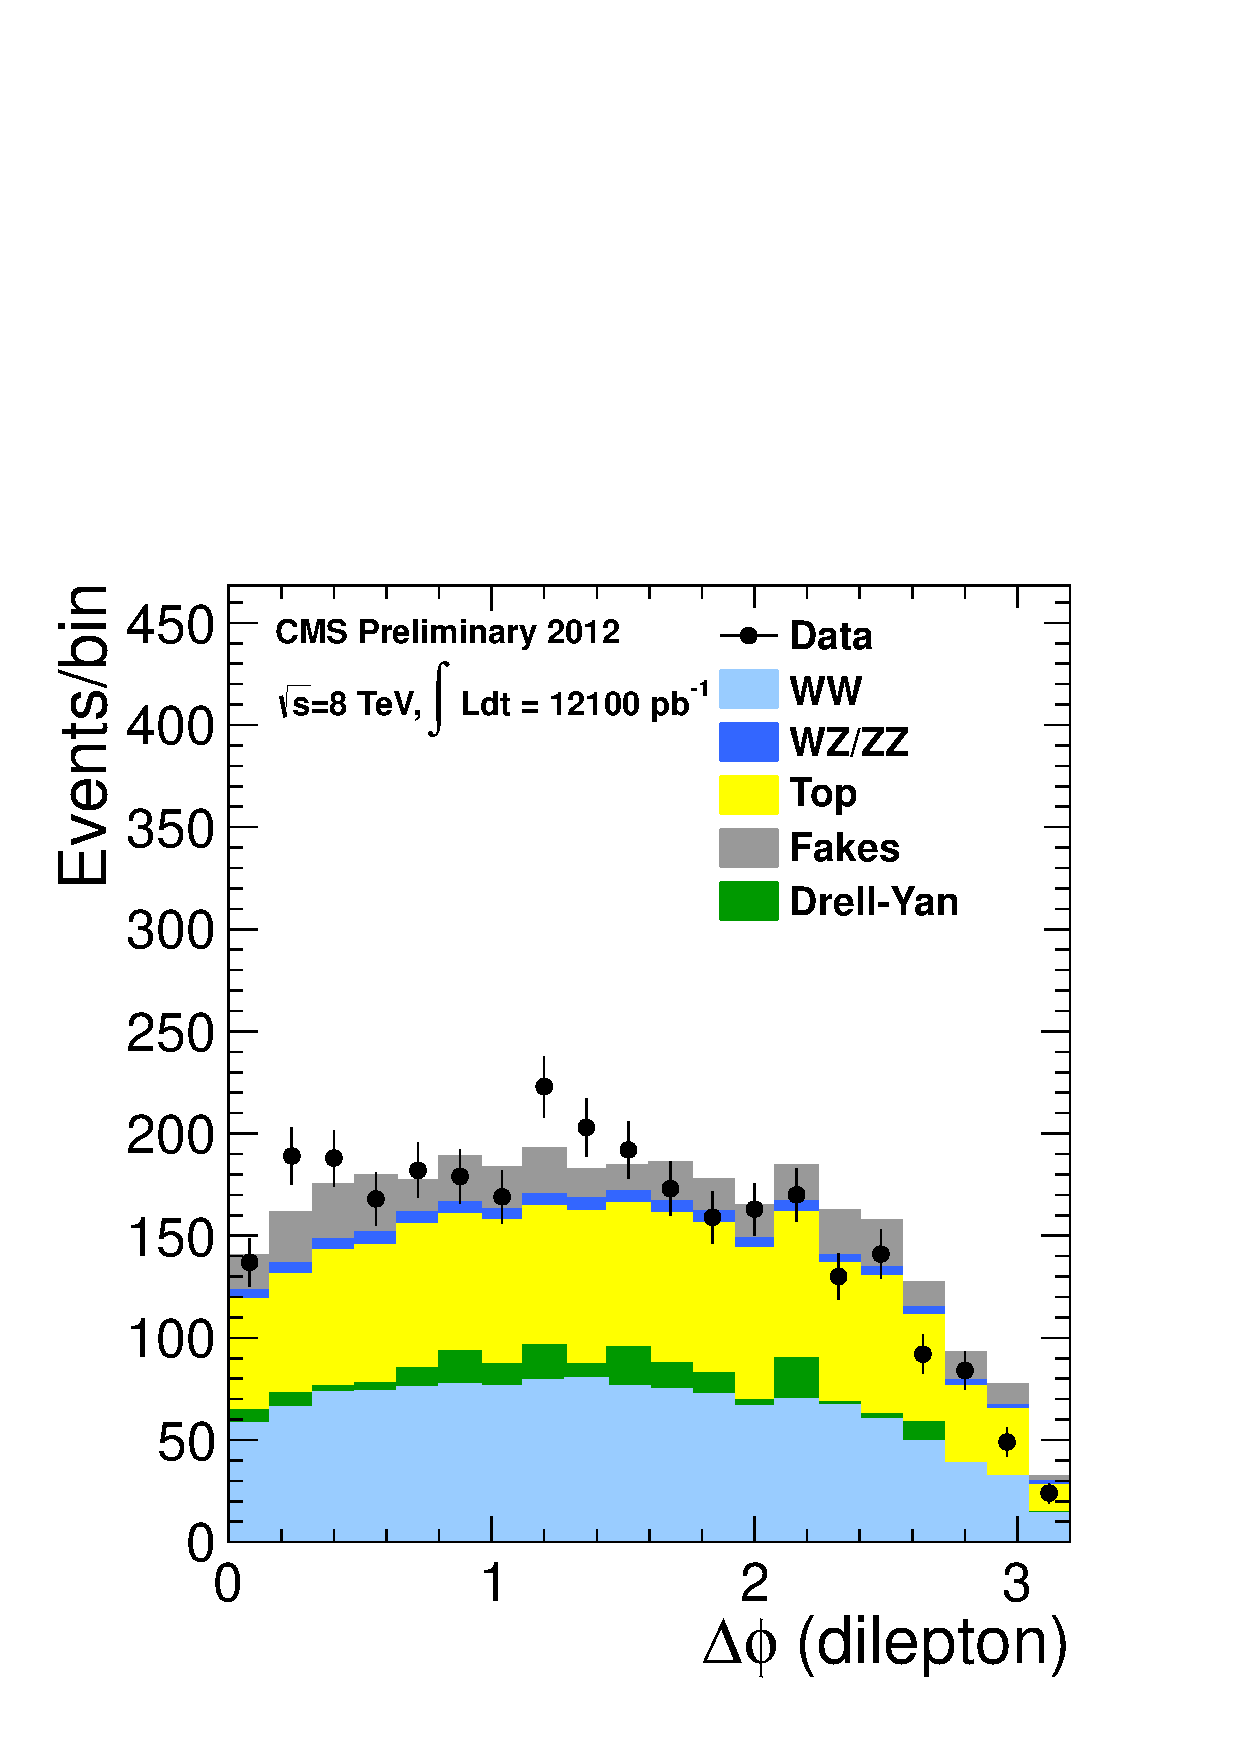
\includegraphics[width=.3\textwidth]{figures/hww_analysis16_0_ALL_incl_1j_dphi.pdf}
}
\subfigure[]{
\centering
\label{subfig:ww_deltaphi_2j}
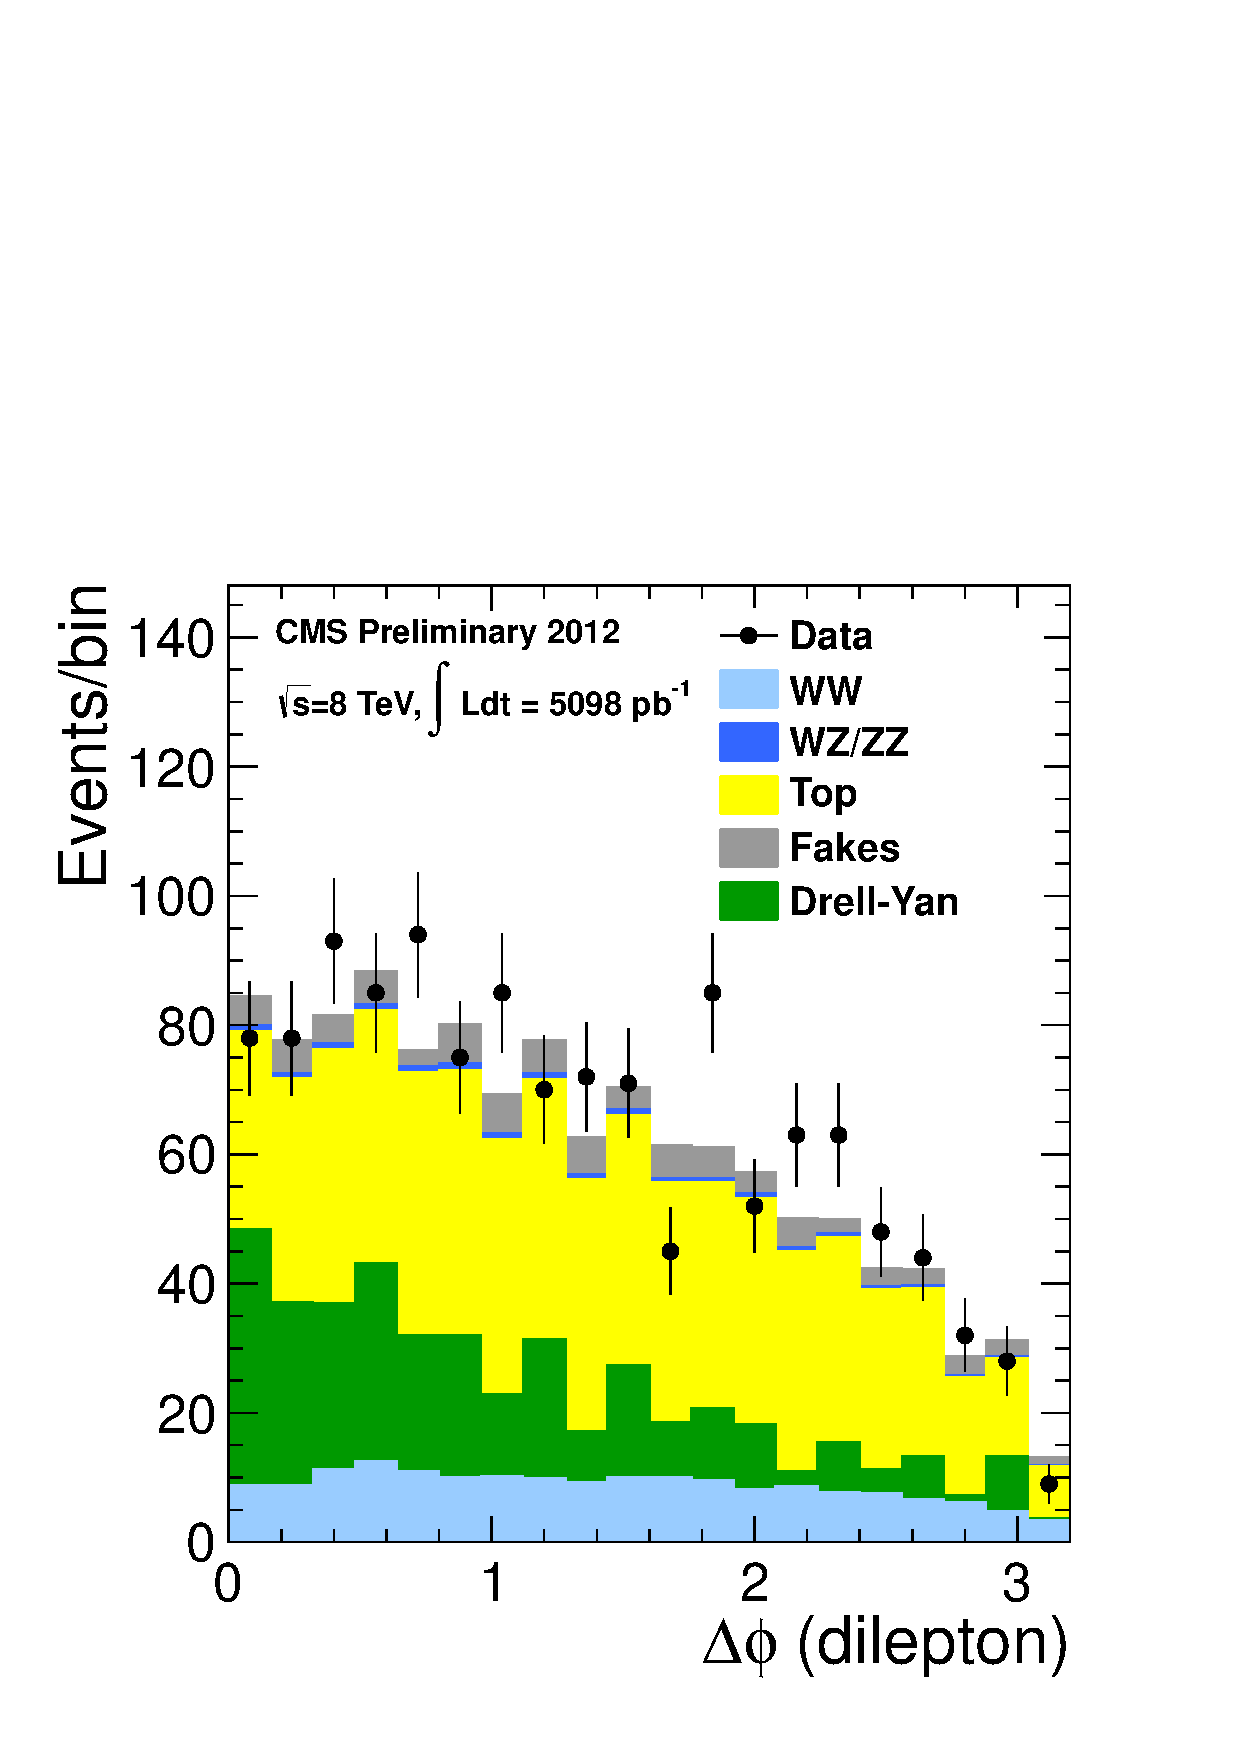
\includegraphics[width=.3\textwidth]{figures/hww_analysis16_0_ALL_incl_2j_dphi.pdf}
} \\
\caption{Dilepton $\Delta\phi$ distribution after WW selection for \intlumiEightTeV of data in the 0-jet \subref{subfig:ww_deltaphi_0j}, 
1-jet \subref{subfig:ww_deltaphi_1j} and 2-jet \subref{subfig:ww_deltaphi_2j} bin analyses. 
MC is scaled to data-driven estimates.}
\label{fig:ww_deltaphi}
\end{figure}

\begin{figure}[!hbtp]
\centering
\subfigure[]{
\centering
\label{subfig:ww_mjj_2j}
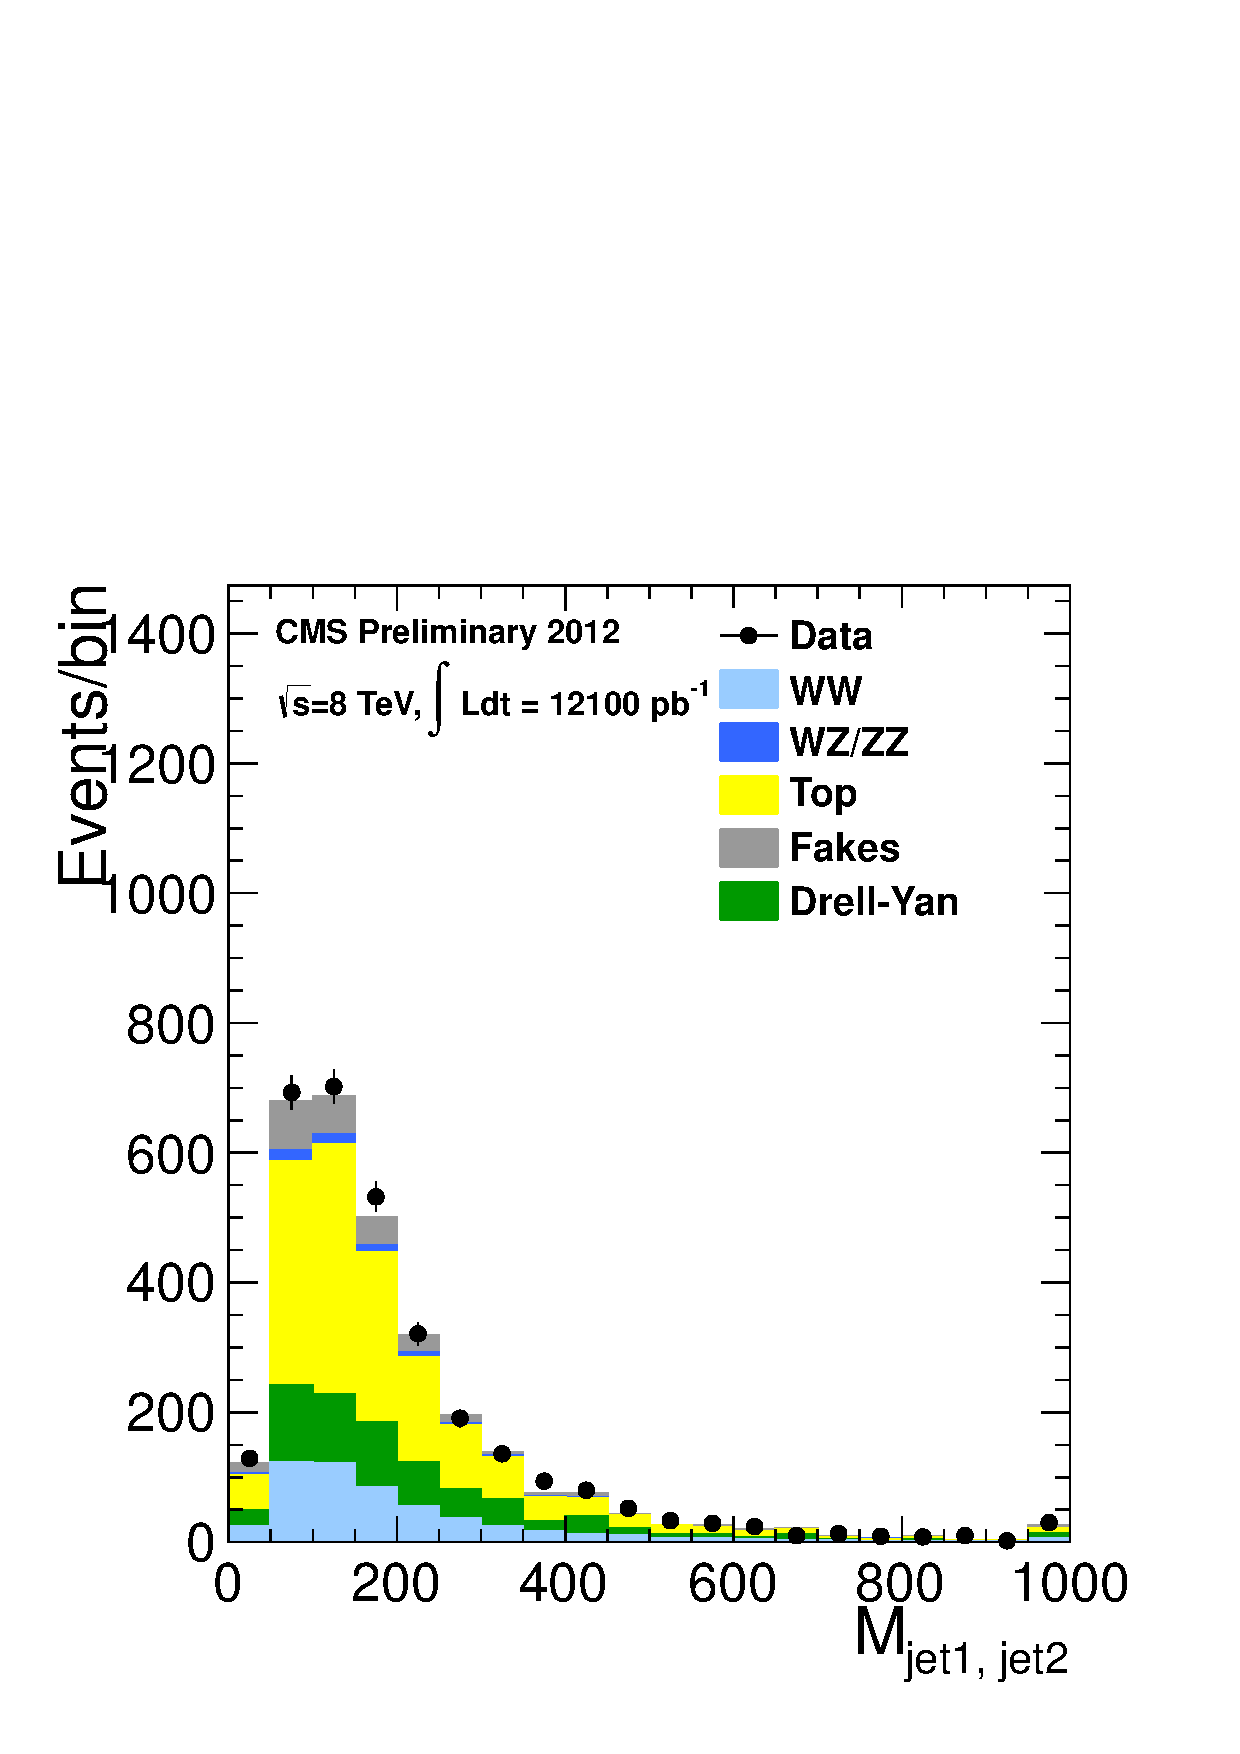
\includegraphics[width=.3\textwidth]{figures/hww_analysis16_0_ALLjj_incl_2j_mjj.pdf}
}
\subfigure[]{
\centering
\label{subfig:ww_detajj_2j}
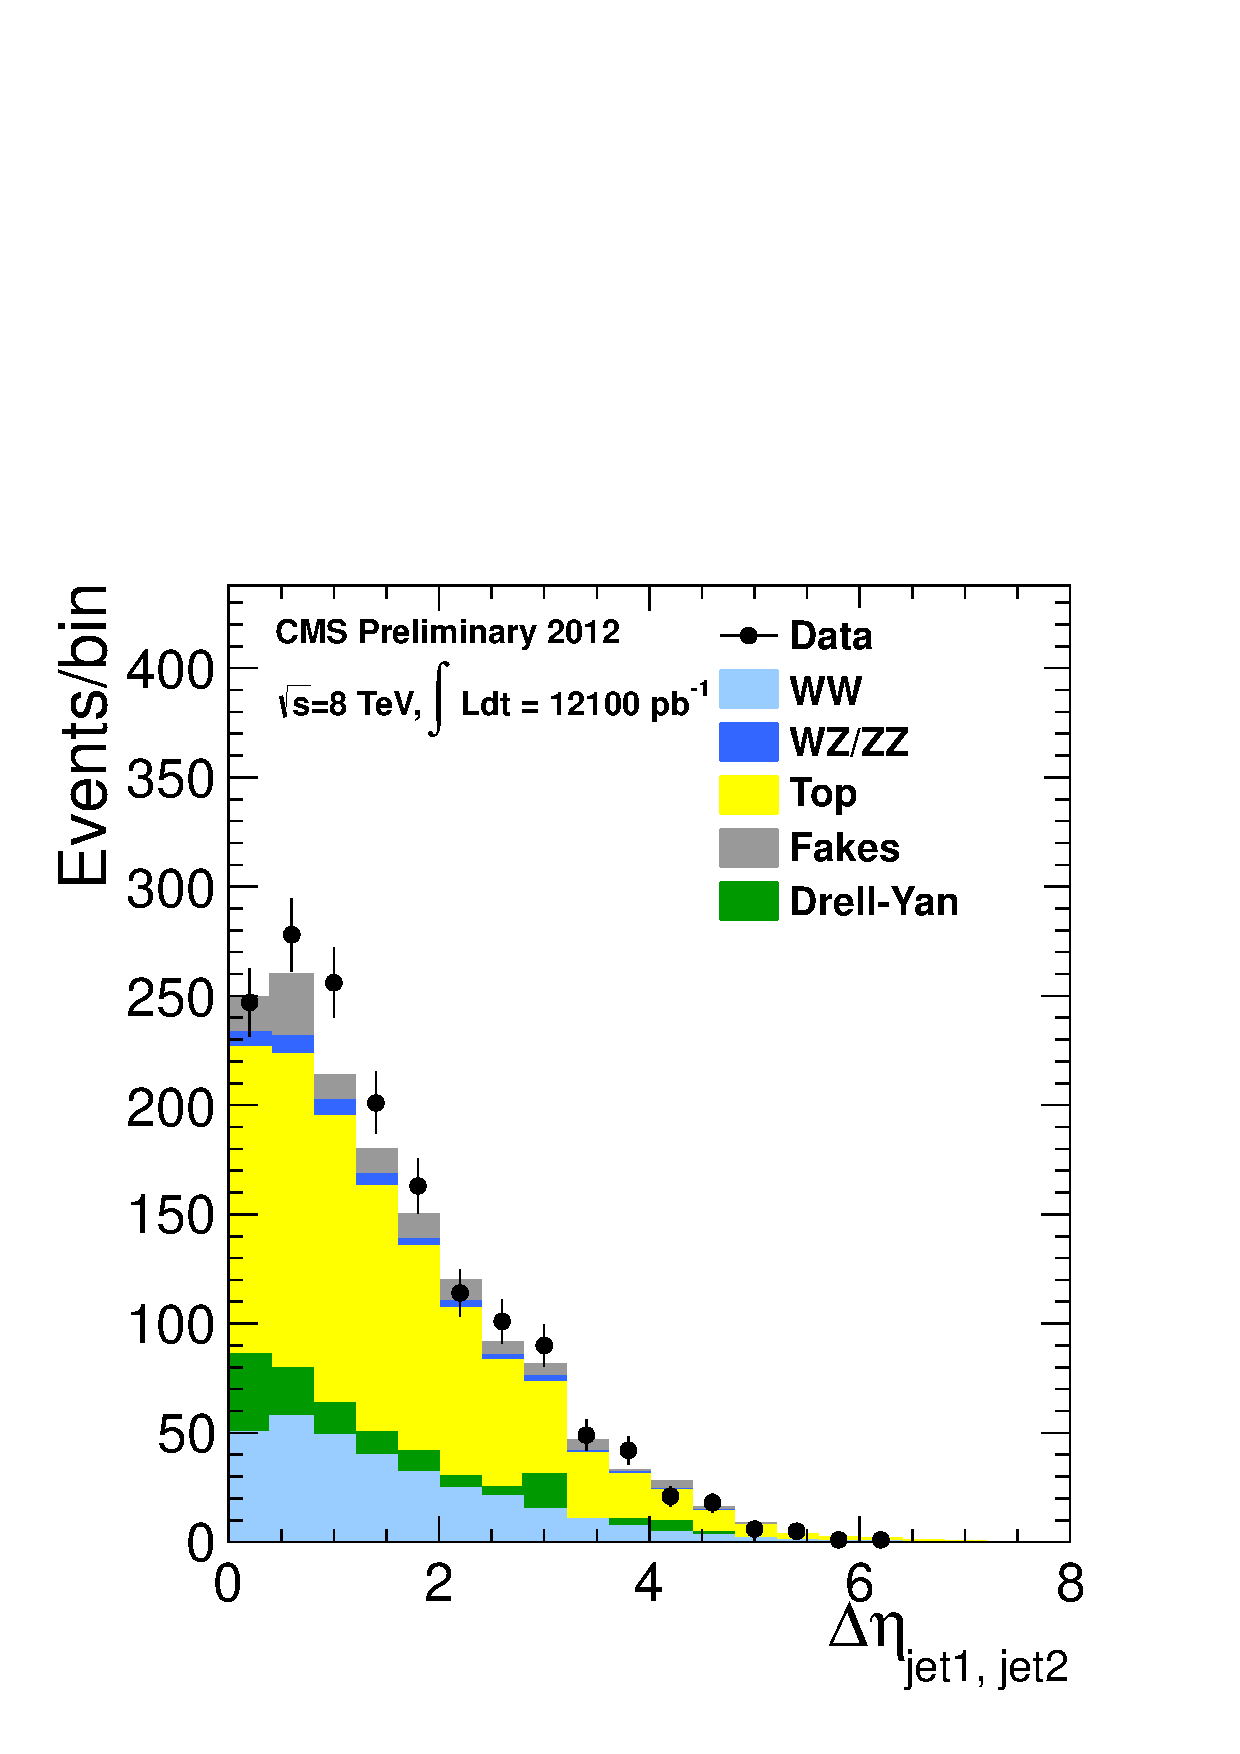
\includegraphics[width=.3\textwidth]{figures/hww_analysis16_0_ALLjj_incl_2j_detajj.pdf}
}
\caption{Di-jet invariant mass \subref{subfig:ww_mjj_2j} and $\Delta\eta(j_1, j_2)$ \subref{subfig:ww_detajj_2j} distributions after the 
WW selection. MC is scaled to data-driven estimates for all processes.}
\label{fig:ww_2j}
\end{figure}

\begin{table}[ht!]
\begin{center}
\begin{tabular}{c | c | c } 
\hline
            & \multicolumn{1}{c|}{0-jet} & \multicolumn{1}{c}{1-jet} \\
mass [\GeV] & scale factor & scale factor \\
\hline
115 &  1.14  $\pm$  0.07  &  0.87  $\pm$  0.12 \\
120 &  1.14  $\pm$  0.07  &  0.87  $\pm$  0.12 \\
125 &  1.14  $\pm$  0.07  &  0.87  $\pm$  0.12 \\
130 &  1.14  $\pm$  0.07  &  0.87  $\pm$  0.12 \\
135 &  1.15  $\pm$  0.07  &  0.88  $\pm$  0.12 \\
140 &  1.14  $\pm$  0.07  &  0.87  $\pm$  0.12 \\
145 &  1.14  $\pm$  0.07  &  0.87  $\pm$  0.12 \\
150 &  1.11  $\pm$  0.07  &  0.87  $\pm$  0.12 \\
155 &  1.11  $\pm$  0.07  &  0.87  $\pm$  0.12 \\
160 &  1.10  $\pm$  0.07  &  0.87  $\pm$  0.12 \\
170 &  1.10  $\pm$  0.07  &  0.87  $\pm$  0.12 \\
180 &  1.10  $\pm$  0.07  &  0.87  $\pm$  0.12 \\
190 &  1.10  $\pm$  0.07  &  0.86  $\pm$  0.12 \\
200 &  1.10  $\pm$  0.07  &  0.86  $\pm$  0.12 \\
\hline
\end{tabular}
\caption{WW background estimation for $\intlumiEightTeV$.}
\label{tab:ww_est_cut}
\end{center}
\end{table}

\begin{table}[ht!]
\begin{center}
\begin{tabular}{c | c } 
\hline
\multicolumn{1}{c|}{0-jet} & \multicolumn{1}{c}{1-jet} \\
scale factor & scale factor \\
\hline
1.23  $\pm$  0.07  &  1.08  $\pm$  0.13 \\
\hline
\end{tabular}
\caption{WW background estimation for $\intlumiEightTeV$.}
\label{tab:ww_est_shape}
\end{center}
\end{table}
%%%%%%%%%%%%%%%%%%%%%%%%%%%%%%

\clearpage
\subsection{Final Results for the Higgs Search with \intlumiEightTeV{}}
\label{sec:search_results}

The expected and observed upper limits at 95\% C.L. for the cut based and
multivariate analyses are shown in Tables~\ref{tab:cutbase_uls}
and~\ref{tab:mvabase_uls}, respectively. The corresponding exclusion
limits are shown in Figure~\ref{fig:uls}. The detailed event yields 
for both analyses are summarized in Appendices.~\ref{app:appendix_cutresults} 
and~\ref{app:appendix_bdtresults}. 
The expected and observed upper limits at 95\% C.L. for the individual channels 
are summarized in Appendices~\ref{app:appendix_limits_bychannel}. 
The results of the shape analysis using the dilepton mass single variable are 
summarized in Appendix~\ref{app:appendix_mll_bdt2011}.
The results of the shape analysis based on the Matrix Element method 
are summarized in Appendix~\ref{app:appendix_me}. 


%%%%%%%%%%%%%%%%%
% plot
\begin{figure}[!hbtp]
\centering
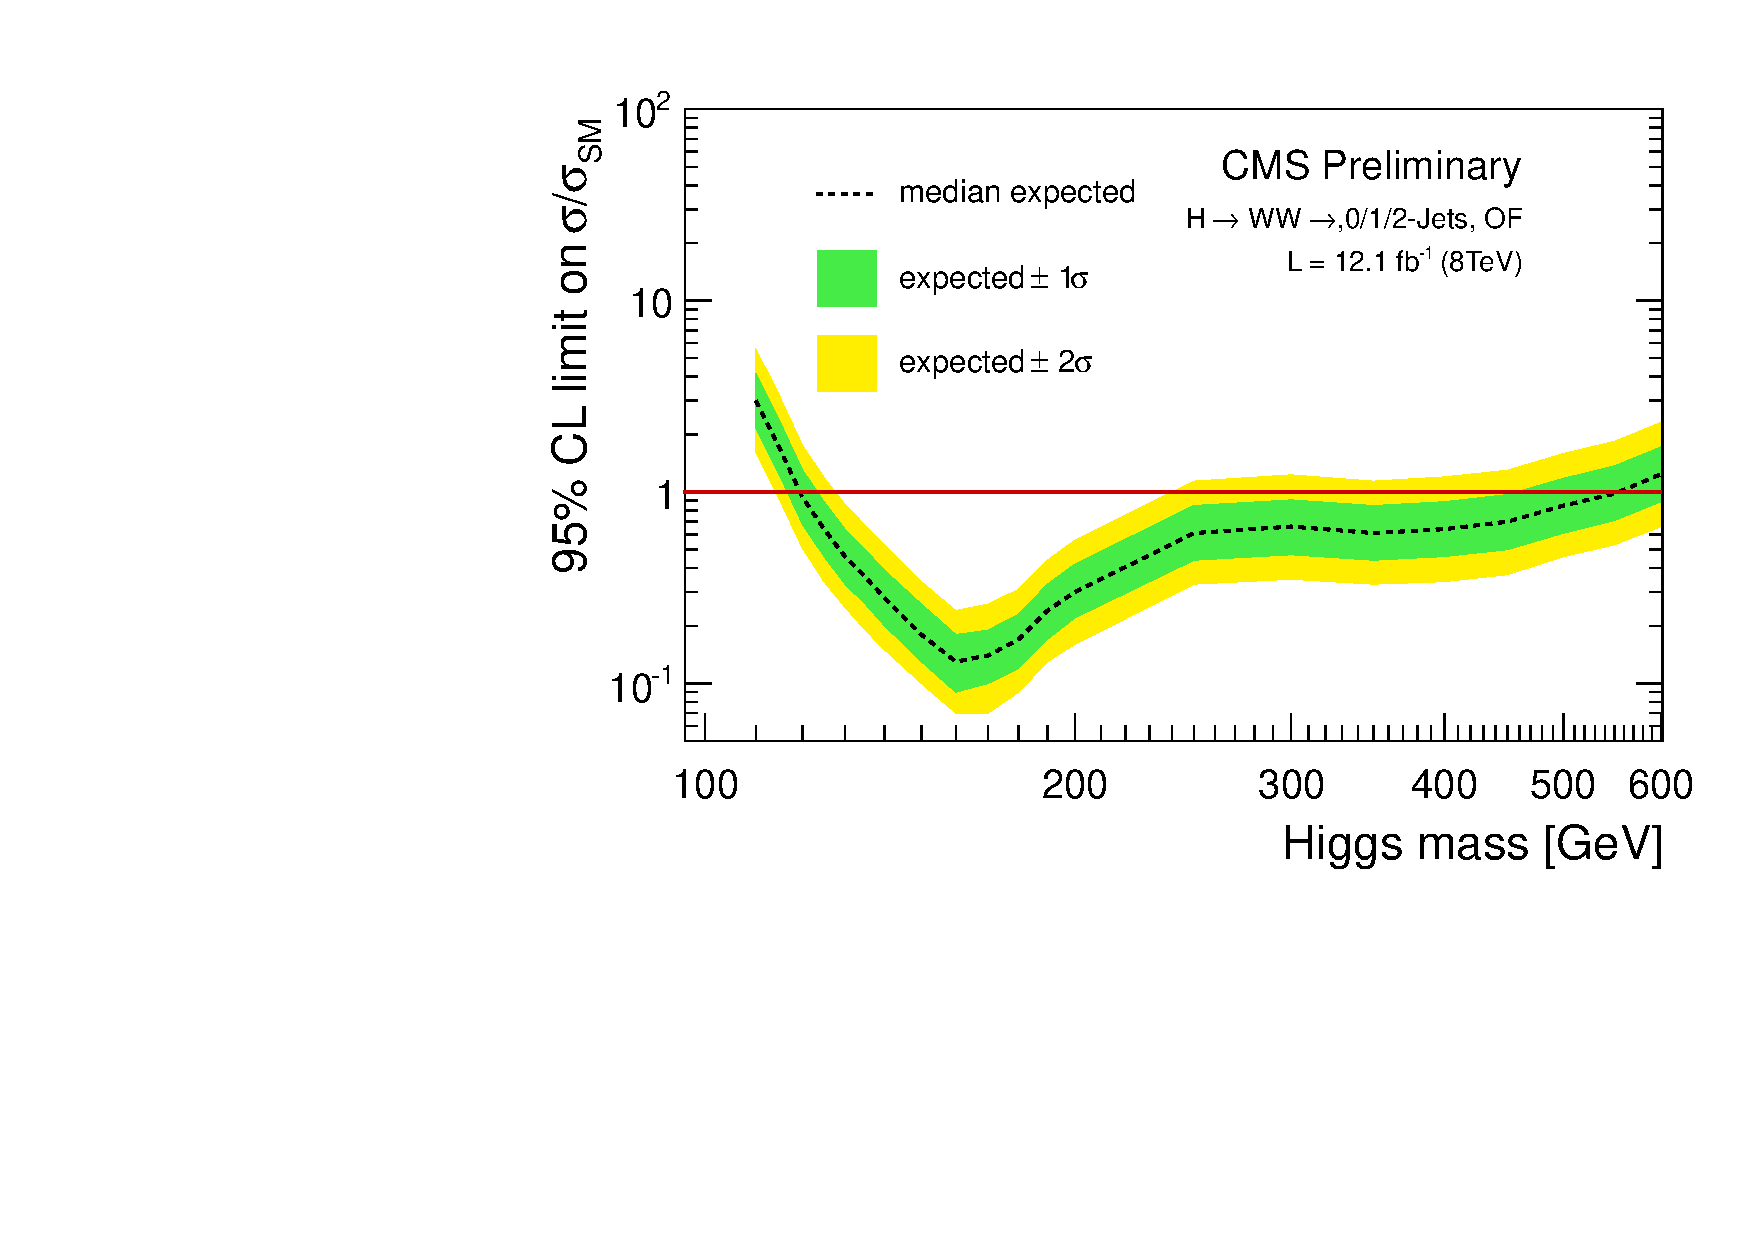
\includegraphics[width=.75\textwidth]{figures/table_limits_nj_shape_of_log.pdf}
\caption{Expected upper limits for SM Higgs in $\intlumiEightTeV$ at 8 TeV in the $e\mu$ channel. 
BDT result is used for 0/1jet bin and cut-based result is used for VBF channel. }
\label{fig:uls_of_bdt01_cut2}
\end{figure}
% table
\begin{table}[!htbp]
\begin{center}
\begin{tabular}{c c c c c}
\hline
\vspace{-3mm} && \\
Higgs Mass & Observed  & Median expected & Expected range for 68\% & Expected range for 95\%   \\
\hline
\vspace{-3mm} && \\
110 & -1.00 & 3.31 & [2.39, 4.61] & [1.78, 6.18] \\
115 & -1.00 & 1.90 & [1.37, 2.64] & [1.02, 3.54] \\
120 & -1.00 & 1.06 & [0.76, 1.48] & [0.57, 1.98] \\
125 & -1.00 & 0.73 & [0.52, 1.01] & [0.39, 1.36] \\
130 & -1.00 & 0.52 & [0.37, 0.72] & [0.28, 0.96] \\
135 & -1.00 & 0.42 & [0.30, 0.58] & [0.22, 0.78] \\
140 & -1.00 & 0.32 & [0.23, 0.44] & [0.17, 0.60] \\
145 & -1.00 & 0.32 & [0.23, 0.44] & [0.17, 0.60] \\
150 & -1.00 & 0.20 & [0.15, 0.28] & [0.11, 0.38] \\
155 & -1.00 & 0.20 & [0.15, 0.28] & [0.11, 0.38] \\
160 & -1.00 & 0.14 & [0.10, 0.19] & [0.07, 0.26] \\
170 & -1.00 & 0.15 & [0.11, 0.21] & [0.08, 0.28] \\
180 & -1.00 & 0.18 & [0.13, 0.26] & [0.10, 0.34] \\
190 & -1.00 & 0.27 & [0.19, 0.37] & [0.14, 0.49] \\
200 & -1.00 & 0.33 & [0.24, 0.46] & [0.18, 0.62] \\
250 & -1.00 & 0.68 & [0.49, 0.95] & [0.36, 1.27] \\
300 & -1.00 & 0.77 & [0.55, 1.07] & [0.41, 1.43] \\
350 & -1.00 & 0.71 & [0.51, 0.99] & [0.38, 1.32] \\
400 & -1.00 & 0.74 & [0.53, 1.02] & [0.39, 1.37] \\
450 & -1.00 & 0.78 & [0.56, 1.09] & [0.42, 1.46] \\
500 & -1.00 & 0.95 & [0.68, 1.32] & [0.51, 1.77] \\
550 & -1.00 & 1.11 & [0.80, 1.54] & [0.59, 2.07] \\
600 & -1.00 & 1.48 & [1.07, 2.06] & [0.80, 2.77] \\
\hline
\end{tabular}
\caption{Expected upper limits for SM Higgs in $\intlumiEightTeV$ at 8 TeV in the $e\mu$ channel. 
BDT result is used for 0/1jet bin and cut-based result is used for VBF channel. }
\label{tab:uls_of_bdt01_cut2}
\end{center}
\end{table} 
%%%%%%%%%%

%%%%%%%%%%%%%%%%%
% plot
\begin{figure}[!hbtp]
\centering
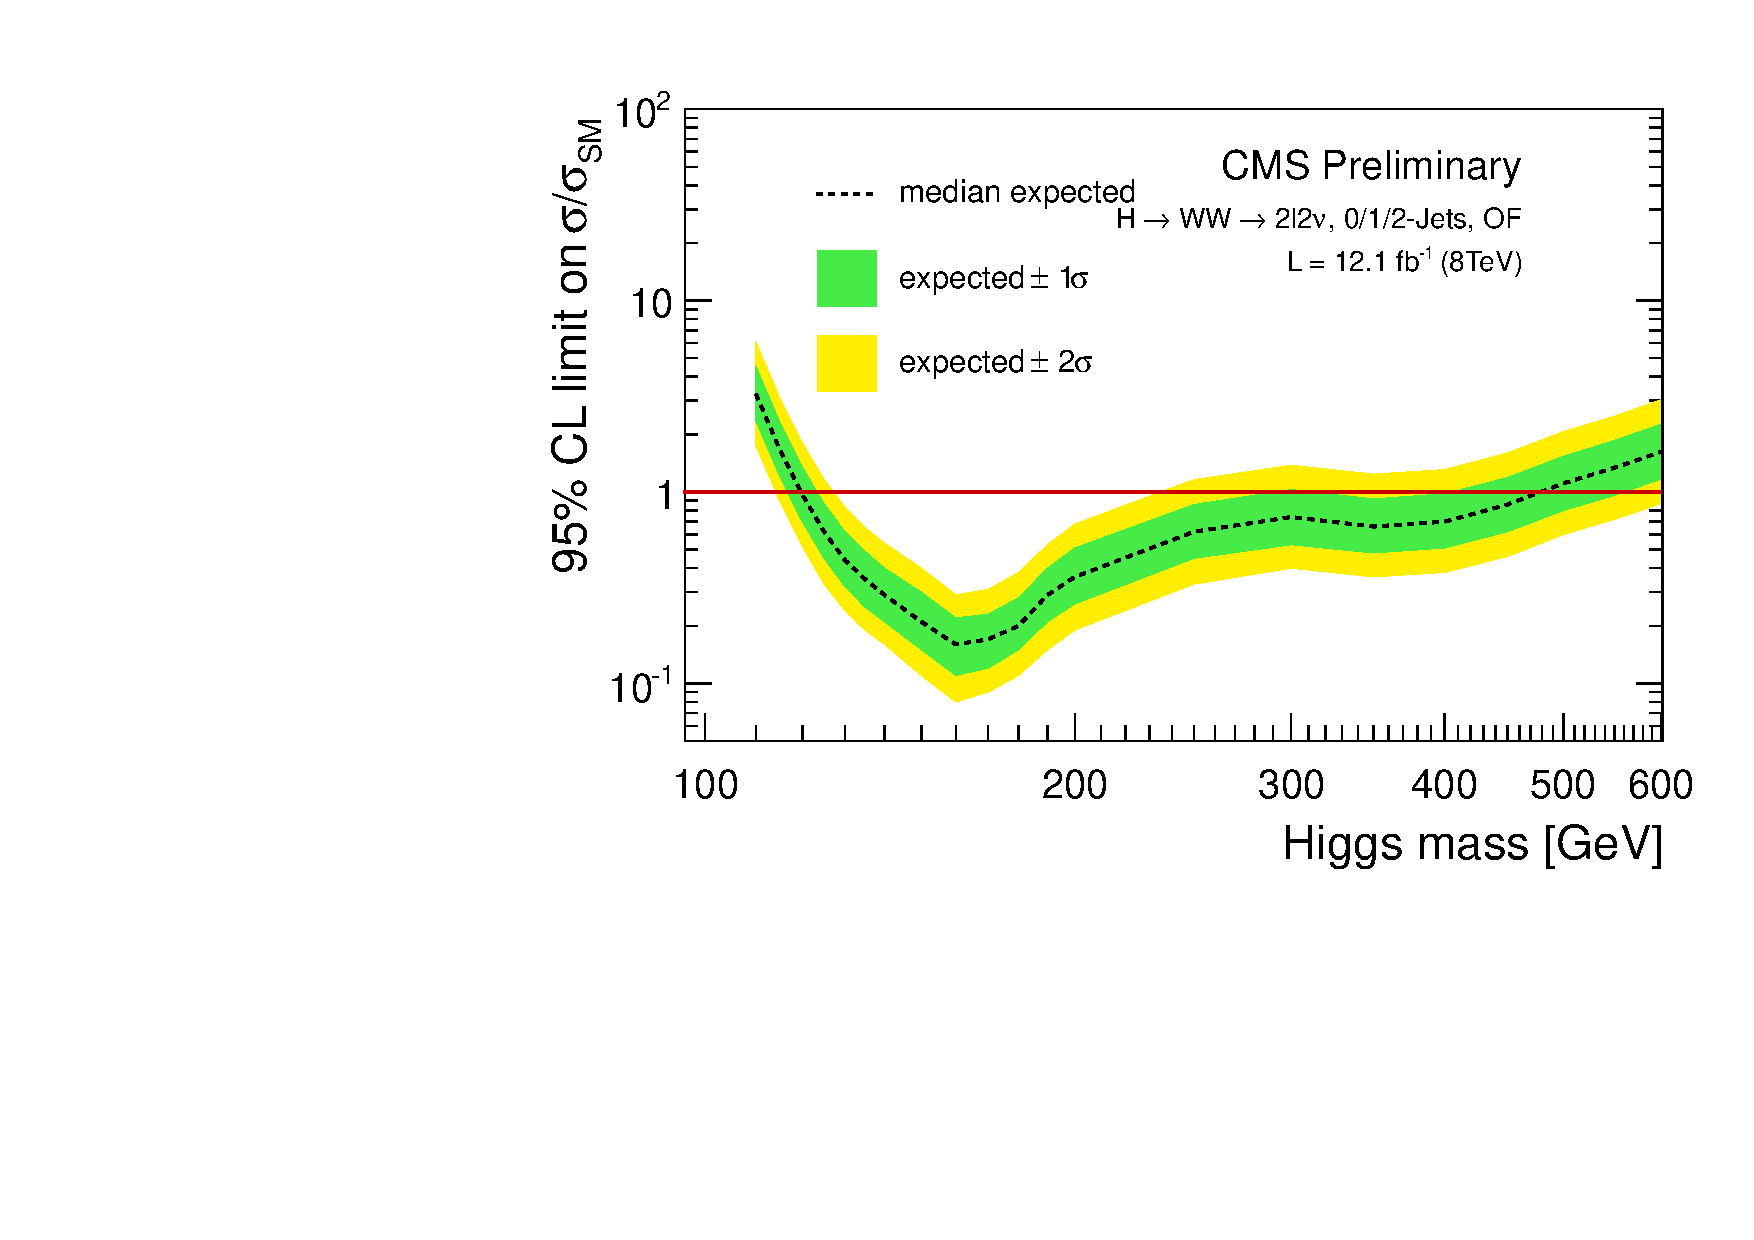
\includegraphics[width=.75\textwidth]{figures/table_limits_nj_shape2d_of_log.pdf}
\caption{Expected upper limits for SM Higgs in $\intlumiEightTeV$ at 8 TeV in the $e\mu$ channel. 
2D result is used for 0/1jet bin and cut-based result is used for VBF channel. }
\label{fig:uls_of_2d01_cut2}
\end{figure}
% table
\begin{table}[!htbp]
\begin{center}
\begin{tabular}{c c c c c}
\hline
\vspace{-3mm} && \\
Higgs Mass & Observed  & Median expected & Expected range for 68\% & Expected range for 95\%   \\
\hline
\vspace{-3mm} && \\
\hline
110 & -1.00 & 3.26 & [2.35, 4.54] & [1.75, 6.09] \\
115 & -1.00 & 1.67 & [1.21, 2.33] & [0.90, 3.12] \\
120 & -1.00 & 0.97 & [0.70, 1.35] & [0.52, 1.81] \\
125 & -1.00 & 0.62 & [0.45, 0.87] & [0.33, 1.16] \\
130 & -1.00 & 0.44 & [0.32, 0.62] & [0.24, 0.83] \\
135 & -1.00 & 0.35 & [0.25, 0.49] & [0.19, 0.65] \\
140 & -1.00 & 0.29 & [0.21, 0.40] & [0.16, 0.54] \\
150 & -1.00 & 0.21 & [0.15, 0.30] & [0.11, 0.40] \\
160 & -1.00 & 0.16 & [0.11, 0.22] & [0.08, 0.29] \\
170 & -1.00 & 0.17 & [0.12, 0.23] & [0.09, 0.31] \\
180 & -1.00 & 0.20 & [0.15, 0.28] & [0.11, 0.38] \\
190 & -1.00 & 0.29 & [0.21, 0.40] & [0.15, 0.53] \\
200 & -1.00 & 0.36 & [0.26, 0.51] & [0.19, 0.68] \\
250 & -1.00 & 0.62 & [0.45, 0.86] & [0.33, 1.16] \\
300 & -1.00 & 0.74 & [0.53, 1.03] & [0.40, 1.38] \\
350 & -1.00 & 0.66 & [0.48, 0.92] & [0.36, 1.24] \\
400 & -1.00 & 0.70 & [0.51, 0.98] & [0.38, 1.31] \\
450 & -1.00 & 0.86 & [0.62, 1.19] & [0.46, 1.60] \\
500 & -1.00 & 1.11 & [0.80, 1.54] & [0.60, 2.07] \\
550 & -1.00 & 1.34 & [0.96, 1.86] & [0.72, 2.49] \\
600 & -1.00 & 1.62 & [1.17, 2.26] & [0.87, 3.03] \\
\end{tabular}
\caption{Expected upper limits for SM Higgs in $\intlumiEightTeV$ at 8 TeV in the $e\mu$ channel. 
2D result is used for 0/1jet bin and cut-based result is used for VBF channel. }
\label{tab:uls_of_2d01_cut2}
\end{center}
\end{table} 
%%%%%%%%%%


%%%%%%%%%%%%%%%%%
% plot
\begin{figure}[!hbtp]
\centering
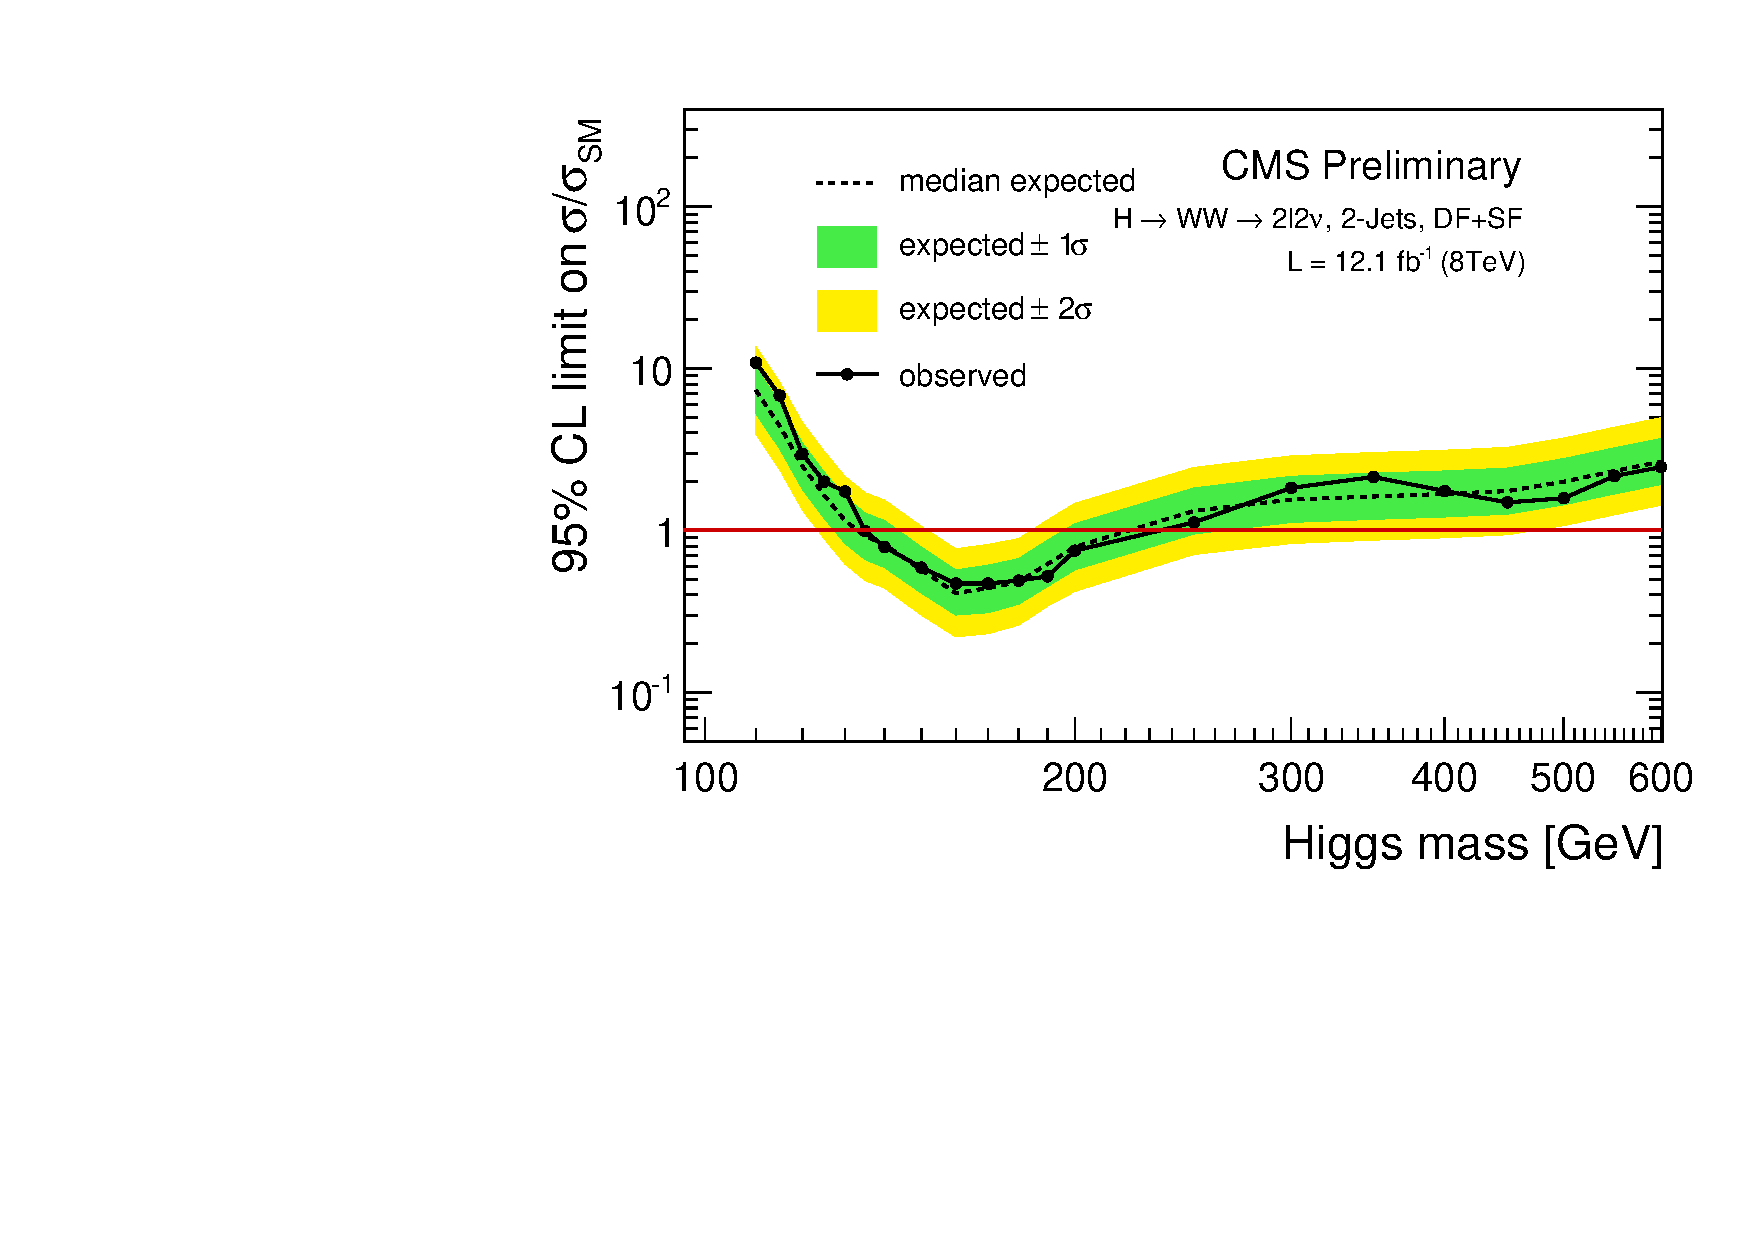
\includegraphics[width=.75\textwidth]{figures/table_limits_2j_cut_log.pdf}
\caption{Expected upper limits for SM Higgs in $\intlumiEightTeV$ at 8 TeV in the VBF channel. 
The cut-based result is used. }
\label{fig:uls_2j_cut}
\end{figure}
% table
\begin{table}[!htbp]
\begin{center}
\begin{tabular}{c c c c c}
\hline
\vspace{-3mm} && \\
Higgs Mass & Observed  & Median expected & Expected range for 68\% & Expected range for 95\%   \\
\hline
110 & -1.00 & 7.95 & [5.73, 11.06] & [4.27, 14.83] \\
115 & -1.00 & 4.67 & [3.37, 6.50] & [2.51, 8.71] \\
120 & -1.00 & 2.60 & [1.88, 3.62] & [1.40, 4.86] \\
125 & -1.00 & 1.74 & [1.25, 2.42] & [0.93, 3.24] \\
130 & -1.00 & 1.19 & [0.85, 1.65] & [0.64, 2.21] \\
135 & -1.00 & 0.96 & [0.70, 1.34] & [0.52, 1.80] \\
140 & -1.00 & 0.82 & [0.59, 1.15] & [0.44, 1.54] \\
150 & -1.00 & 0.57 & [0.41, 0.80] & [0.31, 1.07] \\
160 & -1.00 & 0.41 & [0.30, 0.58] & [0.22, 0.77] \\
170 & -1.00 & 0.44 & [0.32, 0.61] & [0.24, 0.82] \\
180 & -1.00 & 0.49 & [0.35, 0.68] & [0.26, 0.91] \\
190 & -1.00 & 0.63 & [0.45, 0.88] & [0.34, 1.18] \\
200 & -1.00 & 0.81 & [0.58, 1.12] & [0.43, 1.50] \\
250 & -1.00 & 1.36 & [0.98, 1.89] & [0.73, 2.53] \\
300 & -1.00 & 1.57 & [1.13, 2.19] & [0.84, 2.93] \\
350 & -1.00 & 1.67 & [1.20, 2.33] & [0.90, 3.12] \\
400 & -1.00 & 1.78 & [1.28, 2.48] & [0.96, 3.32] \\
450 & -1.00 & 1.85 & [1.33, 2.57] & [0.99, 3.45] \\
500 & -1.00 & 2.15 & [1.55, 2.98] & [1.15, 4.00] \\
550 & -1.00 & 2.53 & [1.82, 3.52] & [1.36, 4.71] \\
600 & -1.00 & 2.95 & [2.13, 4.11] & [1.58, 5.50] \\
\vspace{-3mm} && \\
\hline
\end{tabular}
\caption{Expected upper limits for SM Higgs in $\intlumiEightTeV$ at 8 TeV in the VBF channel. 
The cut-based result is used. }
\label{tab:uls_2j_cut}
\end{center}
\end{table} 
%%%%%%%%%%


%%%%%%%%%%%%%%%%%
% plot
\begin{figure}[!hbtp]
\centering
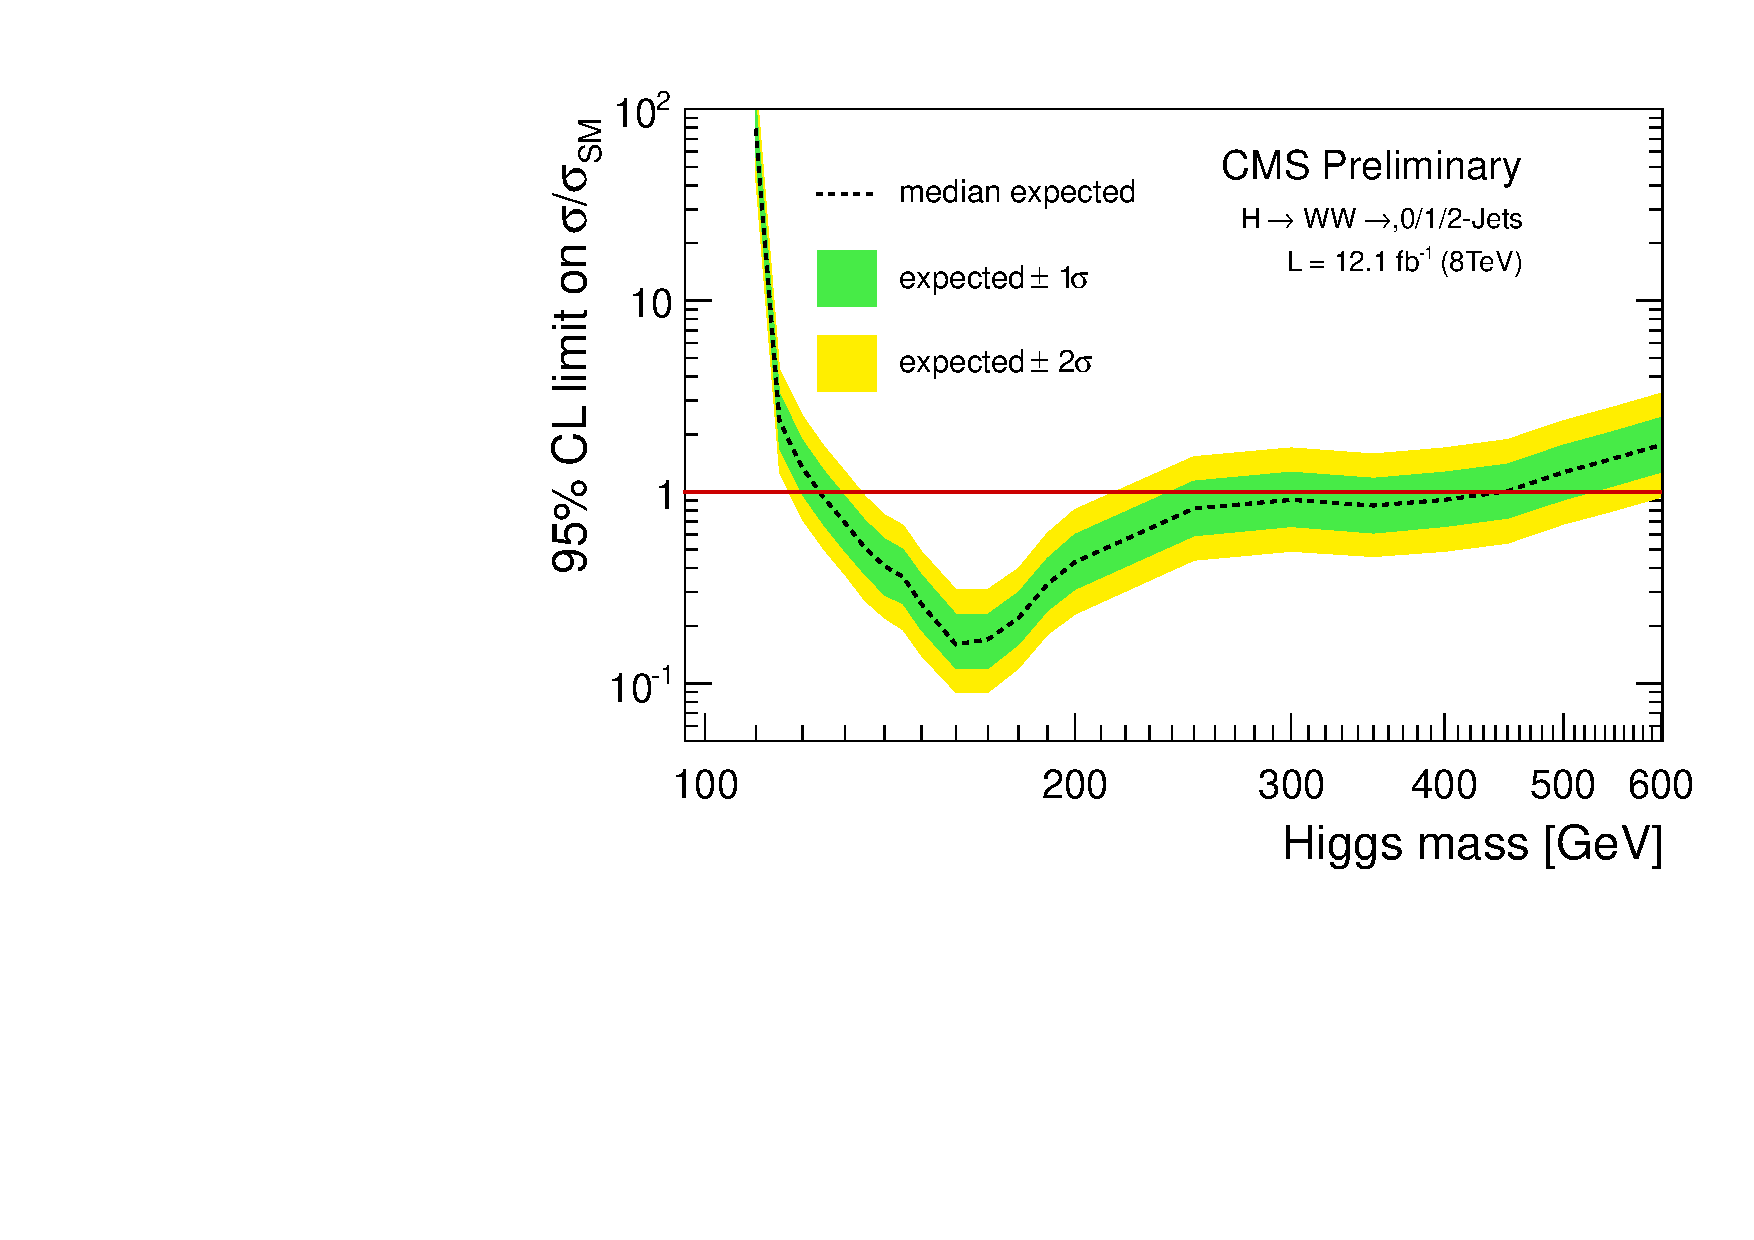
\includegraphics[width=.75\textwidth]{figures/table_limits_nj_cut_log.pdf}
\caption{Expected upper limits for SM Higgs in $\intlumiEightTeV$ at 8 TeV in all final states combined. 
Cut-based result is used. }
\label{fig:uls_cut}
\end{figure}
% table
\begin{table}[!htbp]
\begin{center}
\begin{tabular}{c c c c c}
\hline
\vspace{-3mm} && \\
Higgs Mass & Observed  & Median expected & Expected range for 68\% & Expected range for 95\%   \\
\hline 
110 & -1.00 & 78.80 & [56.77, 109.64] & [42.28, 146.98] \fixme \\ 
115 & -1.00 & 2.34 & [1.69, 3.26] & [1.26, 4.37] \\
120 & -1.00 & 1.34 & [0.97, 1.87] & [0.72, 2.51] \\
125 & -1.00 & 0.93 & [0.67, 1.29] & [0.50, 1.73] \\
130 & -1.00 & 0.69 & [0.49, 0.95] & [0.37, 1.28] \\
135 & -1.00 & 0.51 & [0.37, 0.71] & [0.27, 0.95] \\
140 & -1.00 & 0.41 & [0.29, 0.57] & [0.22, 0.76] \\
145 & -1.00 & 0.36 & [0.26, 0.50] & [0.19, 0.67] \\
150 & -1.00 & 0.26 & [0.19, 0.37] & [0.14, 0.49] \\
155 & -1.00 & 0.26 & [0.19, 0.37] & [0.14, 0.49] \\
160 & -1.00 & 0.16 & [0.12, 0.23] & [0.09, 0.31] \\
170 & -1.00 & 0.17 & [0.12, 0.23] & [0.09, 0.31] \\
180 & -1.00 & 0.22 & [0.16, 0.30] & [0.12, 0.40] \\
190 & -1.00 & 0.33 & [0.24, 0.45] & [0.18, 0.61] \\
200 & -1.00 & 0.43 & [0.31, 0.60] & [0.23, 0.81] \\
250 & -1.00 & 0.82 & [0.59, 1.14] & [0.44, 1.53] \\
300 & -1.00 & 0.91 & [0.66, 1.27] & [0.49, 1.70] \\
350 & -1.00 & 0.85 & [0.61, 1.18] & [0.46, 1.58] \\
400 & -1.00 & 0.91 & [0.66, 1.27] & [0.49, 1.70] \\
450 & -1.00 & 1.01 & [0.73, 1.40] & [0.54, 1.88] \\
500 & -1.00 & 1.27 & [0.91, 1.76] & [0.68, 2.36] \\
550 & -1.00 & 1.50 & [1.08, 2.08] & [0.80, 2.79] \\
600 & -1.00 & 1.76 & [1.27, 2.45] & [0.94, 3.28] \\
\vspace{-3mm} && \\
\hline
\end{tabular}
\caption{Expected upper limits for SM Higgs in $\intlumiEightTeV$ at 8 TeV in all final states combined. 
Cut-based result is used. }
\label{tab:ulscut}
\end{center}
\end{table} 
%%%%%%%%%%

%%%%%%%%%%%%%%%%%
% plot
\begin{figure}[!hbtp]
\centering
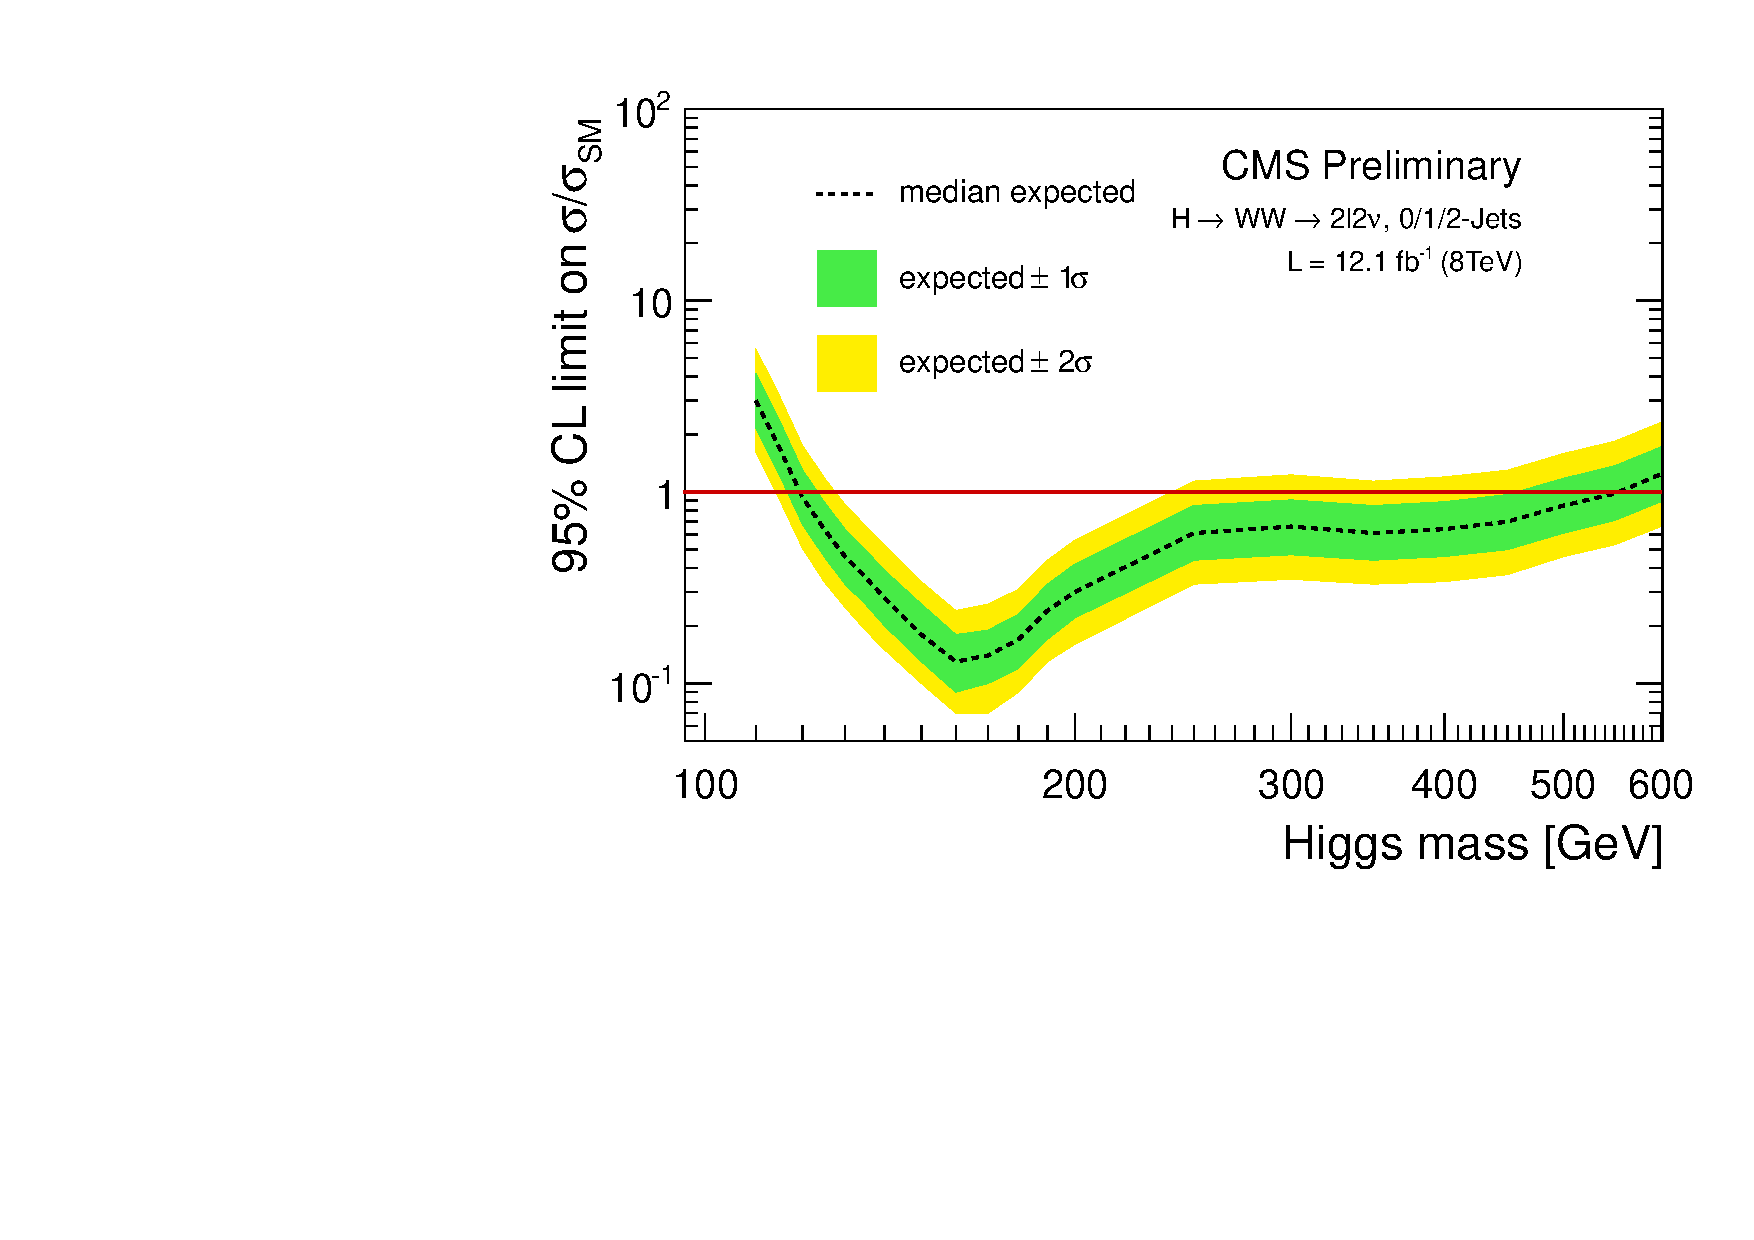
\includegraphics[width=.75\textwidth]{figures/table_limits_nj_shape_of_cut_log.pdf}
\caption{Expected upper limits for SM Higgs in $\intlumiEightTeV$ at 8 TeV. 
BDT result is used for OF 0/1jet bin and cut-based result is used for VBF channel 
and in the SF final states. }
\label{fig:uls_bdt01_cut2_cutsf}
\end{figure}
% table
\begin{table}[!htbp]
\begin{center}
\begin{tabular}{c c c c c}
\hline
\vspace{-3mm} && \\
Higgs Mass & Observed  & Median expected & Expected range for 68\% & Expected range for 95\%   \\
\hline
110 & -1.00 & 3.00 & [2.16, 4.18] & [1.61, 5.60] \\
115 & -1.00 & 1.70 & [1.22, 2.36] & [0.91, 3.17] \\
120 & -1.00 & 0.94 & [0.68, 1.31] & [0.51, 1.76] \\
125 & -1.00 & 0.64 & [0.46, 0.89] & [0.34, 1.19] \\
130 & -1.00 & 0.46 & [0.33, 0.64] & [0.25, 0.86] \\
135 & -1.00 & 0.36 & [0.26, 0.50] & [0.19, 0.67] \\
140 & -1.00 & 0.28 & [0.20, 0.39] & [0.15, 0.53] \\
145 & -1.00 & 0.40 & [0.29, 0.56] & [0.22, 0.76] \\
150 & -1.00 & 0.18 & [0.13, 0.26] & [0.10, 0.34] \\
155 & -1.00 & 0.18 & [0.13, 0.26] & [0.10, 0.34] \\
160 & -1.00 & 0.13 & [0.09, 0.18] & [0.07, 0.24] \\
170 & -1.00 & 0.14 & [0.10, 0.19] & [0.07, 0.26] \\
180 & -1.00 & 0.17 & [0.12, 0.23] & [0.09, 0.31] \\
190 & -1.00 & 0.24 & [0.17, 0.33] & [0.13, 0.44] \\
200 & -1.00 & 0.30 & [0.22, 0.42] & [0.16, 0.56] \\
250 & -1.00 & 0.61 & [0.44, 0.85] & [0.33, 1.14] \\
300 & -1.00 & 0.66 & [0.47, 0.91] & [0.35, 1.23] \\
350 & -1.00 & 0.61 & [0.44, 0.85] & [0.33, 1.14] \\
400 & -1.00 & 0.64 & [0.46, 0.89] & [0.34, 1.20] \\
450 & -1.00 & 0.70 & [0.50, 0.97] & [0.37, 1.30] \\
500 & -1.00 & 0.85 & [0.61, 1.18] & [0.46, 1.59] \\
550 & -1.00 & 0.98 & [0.71, 1.37] & [0.53, 1.84] \\
600 & -1.00 & 1.24 & [0.89, 1.72] & [0.66, 2.31] \\
\vspace{-3mm} && \\
\hline
\end{tabular}
\caption{Expected upper limits for SM Higgs in $\intlumiEightTeV$ at 8 TeV. 
BDT result is used for OF 0/1jet bin and cut-based result is used for VBF channel 
and in the SF final states. }
\label{tab:uls_bdt01_cut2_cutsf}
\end{center}
\end{table} 
%%%%%%%%%%

%%%%%%%%%%%%%%%%%
% plot
\begin{figure}[!hbtp]
\centering
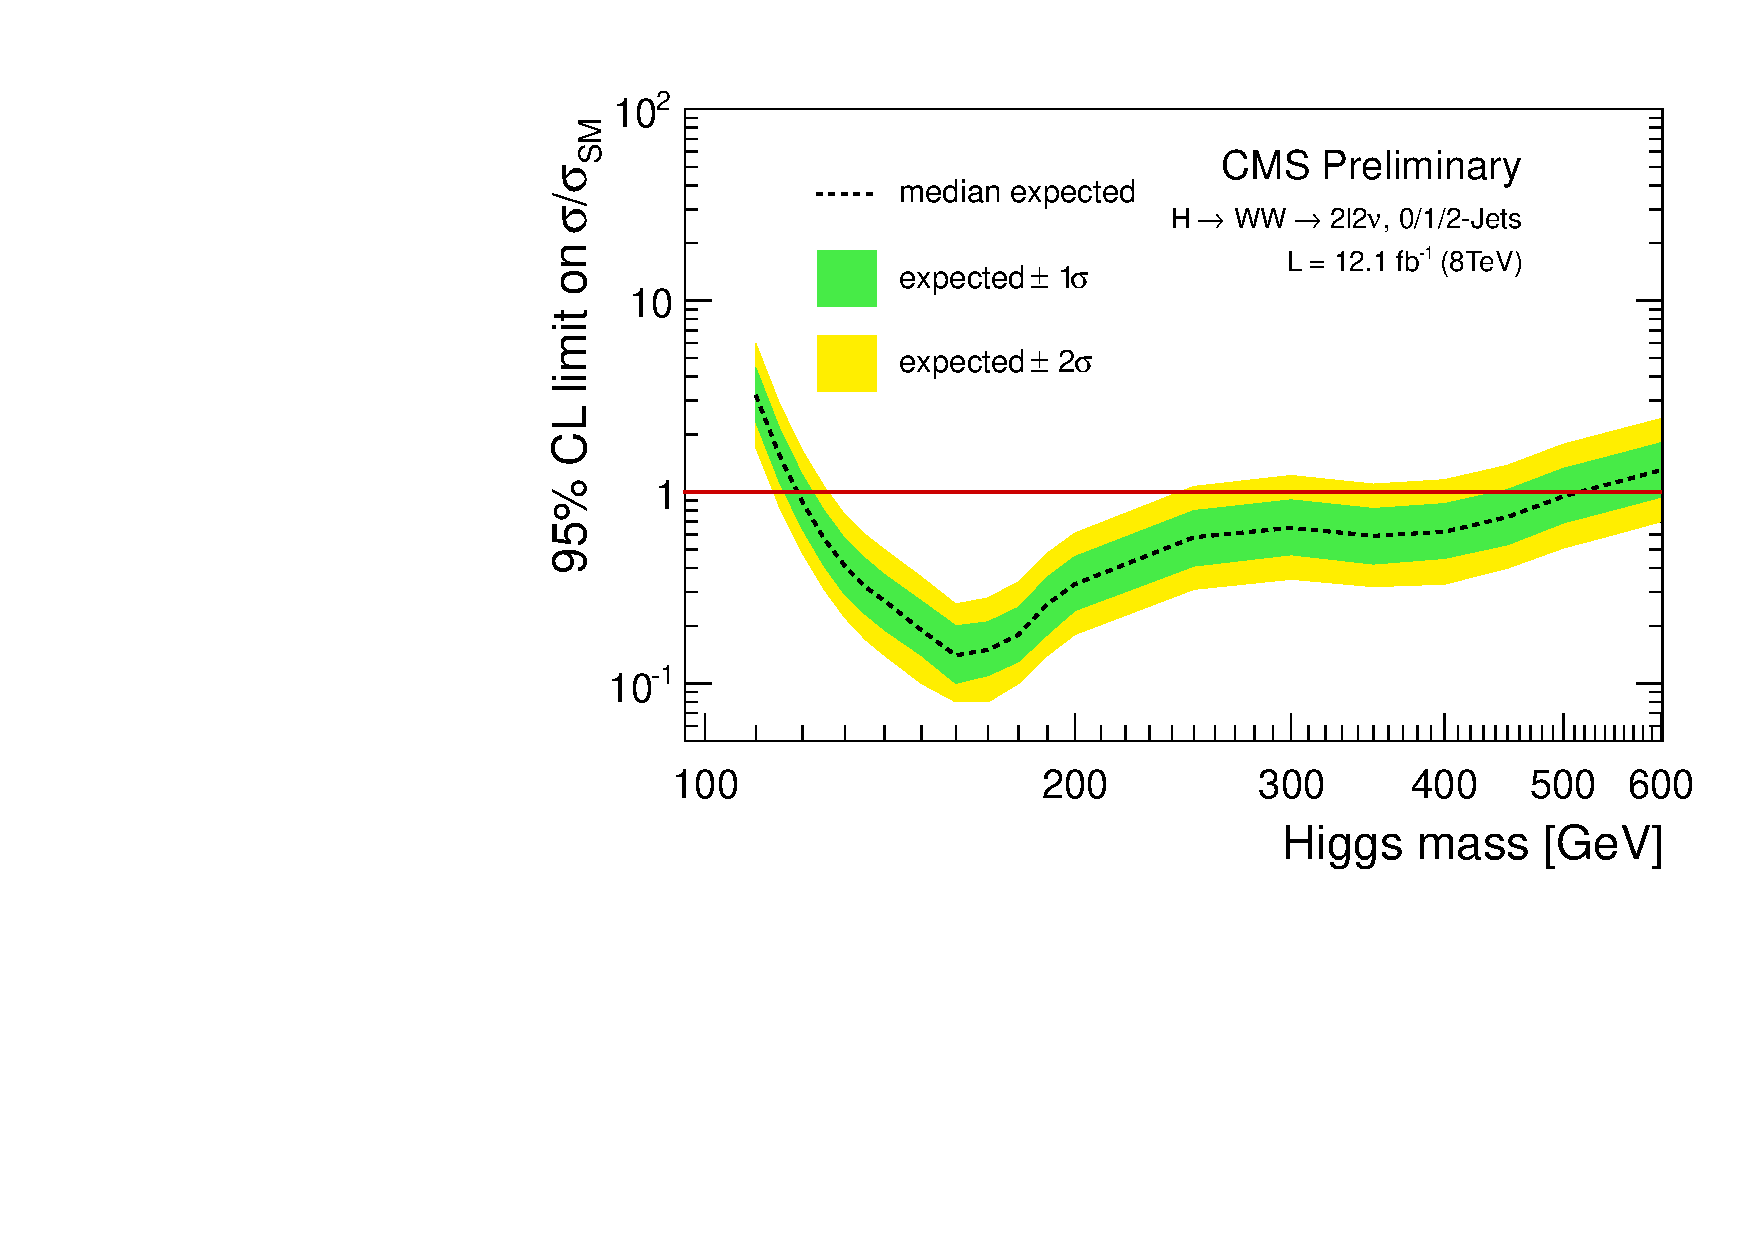
\includegraphics[width=.75\textwidth]{figures/table_limits_nj_shape2d_of_cut_log.pdf}
\caption{Expected upper limits for SM Higgs in $\intlumiEightTeV$ at 8 TeV. 
2D result is used for OF 0/1jet bin and cut-based result is used for VBF channel 
and in the SF final states. }
\label{fig:uls_2d01_cut2_cutsf}
\end{figure}
% table
\begin{table}[!htbp]
\begin{center}
\begin{tabular}{c c c c c}
\hline
\vspace{-3mm} && \\
Higgs Mass & Observed  & Median expected & Expected range for 68\% & Expected range for 95\%   \\
\hline
110 & -1.00 & 64.05 & [46.14, 89.12] & [34.37, 119.47] \fixme  \\
115 & -1.00 & 1.55 & [1.12, 2.15] & [0.83, 2.89] \\
120 & -1.00 & 0.89 & [0.64, 1.23] & [0.48, 1.65] \\
125 & -1.00 & 0.57 & [0.41, 0.80] & [0.31, 1.07] \\
130 & -1.00 & 0.41 & [0.29, 0.57] & [0.22, 0.76] \\
135 & -1.00 & 0.32 & [0.23, 0.45] & [0.17, 0.60] \\
140 & -1.00 & 0.27 & [0.19, 0.37] & [0.14, 0.50] \\
145 & -1.00 & 0.40 & [0.29, 0.56] & [0.22, 0.76] \\
150 & -1.00 & 0.19 & [0.14, 0.27] & [0.10, 0.36] \\
155 & -1.00 & 0.19 & [0.14, 0.27] & [0.10, 0.36] \\
160 & -1.00 & 0.14 & [0.10, 0.20] & [0.08, 0.26] \\
170 & -1.00 & 0.15 & [0.11, 0.21] & [0.08, 0.28] \\
180 & -1.00 & 0.18 & [0.13, 0.25] & [0.10, 0.34] \\
190 & -1.00 & 0.26 & [0.18, 0.36] & [0.14, 0.48] \\
200 & -1.00 & 0.33 & [0.24, 0.46] & [0.18, 0.61] \\
250 & -1.00 & 0.58 & [0.41, 0.80] & [0.31, 1.07] \\
300 & -1.00 & 0.65 & [0.47, 0.91] & [0.35, 1.22] \\
350 & -1.00 & 0.59 & [0.42, 0.82] & [0.32, 1.10] \\
400 & -1.00 & 0.62 & [0.45, 0.87] & [0.33, 1.16] \\
450 & -1.00 & 0.74 & [0.53, 1.03] & [0.40, 1.38] \\
500 & -1.00 & 0.95 & [0.69, 1.33] & [0.51, 1.78] \\
550 & -1.00 & 1.12 & [0.81, 1.56] & [0.60, 2.09] \\
600 & -1.00 & 1.30 & [0.94, 1.81] & [0.70, 2.42] \\
\vspace{-3mm} && \\
\hline
\end{tabular}
\caption{Expected upper limits for SM Higgs in $\intlumiEightTeV$ at 8 TeV. 
2D result is used for OF 0/1jet bin and cut-based result is used for VBF channel 
and in the SF final states. }
\label{tab:uls_2d01_cut2_cutsf}
\end{center}
\end{table} 
%%%%%%%%%%

We also calculate the expected significance.
Results are summarized in Table~\ref{tab:significance_8TeV}.

\begin{table}[!htbp]
\begin{center}
\begin{tabular}{c | c c c c c c }
\hline 
\vspace{-3mm} && \\
Higgs Mass(\GeV) & (1) & (2) & (3) & (4) & (5) & (6)  \\
\hline \hline
115 & 1.2  	& 1.2 	& 0.6 & 1.0 	& 1.3	& 1.3 	\\
125 & 2.7  	& 3.1  	& 1.4 & 2.3		& 3.1	& 3.4	\\
140 & 6.2  	& 6.7 	& 2.5 & 4.7 	& 7.2	& 7.4 	\\
160 & 16.6 	& 14.3  & 4.1 & 11.2	& 18.4	& 16.1	\\
200 & 5.8 	& 5.4  	& 2.2 & 4.4 	& 6.4	& 6.0	\\
400 & 2.8 	& 2.7 	& 1.0 & 2.1		& 3.2	& 3.1	\\
600 & 1.4  	& 1.2 	& 0.7 & 1.2		& 1.7	& 1.5	\\
\hline
\end{tabular}
\caption{Expected significance SM Higgs in $\intlumiEightTeV$ at 8 TeV. (1) is BDT 0/1j OF + cut 2j OF. (2) is 2D 0/1j OF+ cut 2j OF. (3) is VBF cut SF+OF. (4) is cut OF+SF. (5) is BDT 0/1j OF + cut 2j OF + cut SF. (6) is 2D 0/1j OF + cut 2j OF + cut SF.} 
\label{tab:significance_8TeV}
\end{center}
\end{table} 

%%%%%%%%%%%%%%%%%%%%%%%%%%%%%%




%%%%%%%%%%%
\clearpage 

\subsection{Final Results for the Higgs Search Combing 7 TeV and 8 TeV Data}
\label{sec:search_results_finalcomb}

In this section we document the Higgs search results combining the 7 \TeV\ and 8 \TeV\ data.  
For the 0 and 1 Jet bin final states, the 7 TeV analysis uses the shape based approach for all 
lepton flavor final states, while the 8 TeV analysis uses the shape based approach only 
in the $e\mu$ channel. 
The expected and observed upper limits at 95\% C.L. are shown in Figure~\ref{fig:uls_finalcomb_shape} 
and Table~\ref{tab:uls_finalcomb_shape}.  We also calculate the expected significance in Table~\ref{tab:significance_78TeV}. 

\begin{figure}[!hbtp]
\centering
%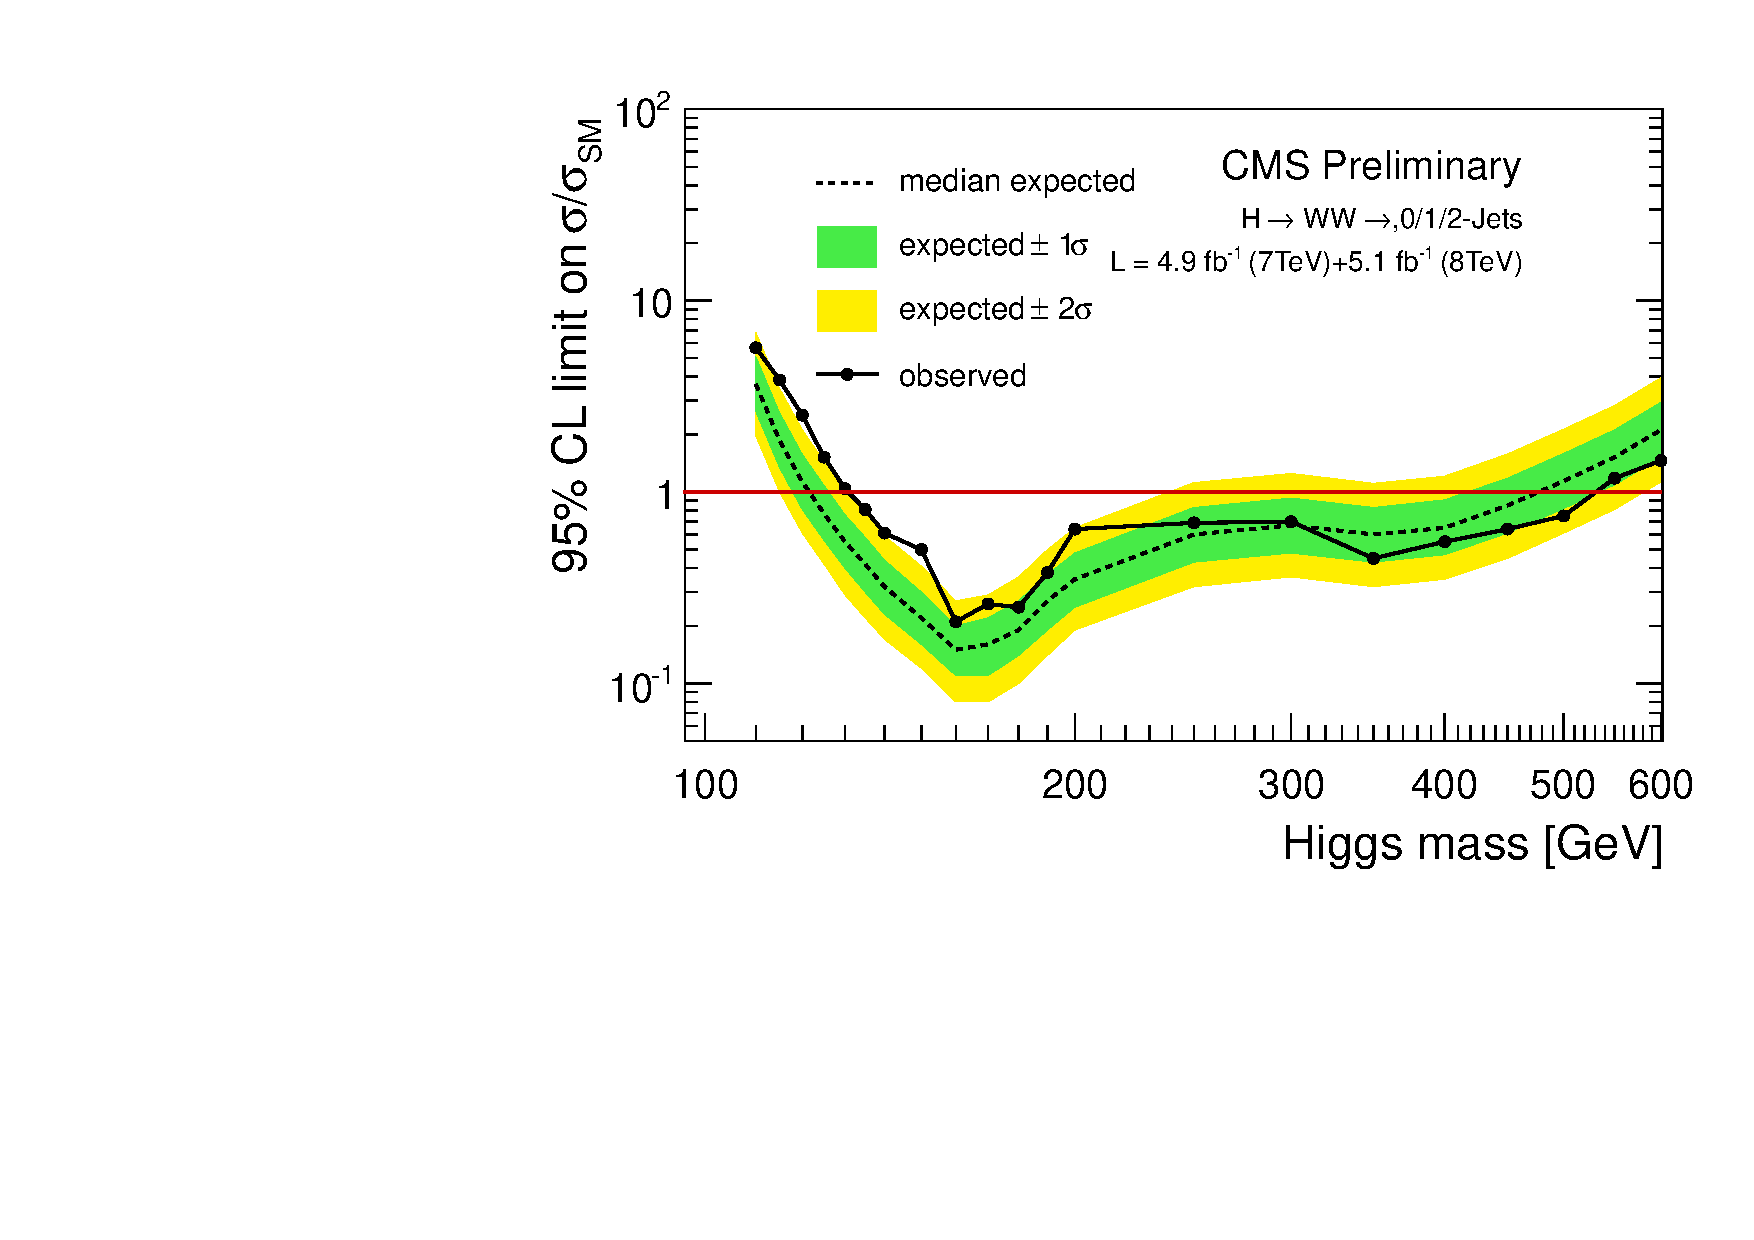
\includegraphics[width=.75\textwidth]{figures/ana_ICHEP2012_finalcomb-CLs-asymptotic_log.pdf}
\caption{Expected and observed upper limits for SM Higgs combining the $\intlumiSevenTeV$ data
at 7 TeV and the $\intlumiEightTeV$ at 8 TeV.
For the 0 and 1 Jet bin final states, the 7 TeV analysis uses the shape based approach for all
lepton flavor final states, while the 8 TeV analysis uses the shape based approach only
in the $e\mu$ channel.
}
\label{fig:uls_finalcomb_shape}
\end{figure}


Appendix~\ref{app:appendix_limits_combination7and8} documents the 
results combining the shape based approach in 7 TeV and the cut based approach in 8 TeV, as shown 
in the ICHEP 2012 conference. 

\begin{table}[!htbp]
\begin{center}
\begin{tabular}{c | c c c  }
\hline 
\vspace{-3mm} && \\
Higgs Mass(\GeV) & (1) & (2) & (3) \\
\hline \hline
115 &  x	& x 	& x \\
125 &  x 	& x  	& x \\
140 &  x 	& x 	& x \\
160 &  x	& x 	& x	\\
200 &  x	& x 	& x	\\
400 &  x	& x 	& x \\
600 &  x	& x		& x \\
\hline
\end{tabular}
\caption{Expected significance for SM Higgs combining the $\intlumiSevenTeV$ data
at 7 TeV and the $\intlumiEightTeV$ at 8 TeV. 
For the 0 and 1 Jet bin final states, the 7 TeV analysis uses the shape based approach for all
lepton flavor final states. For (1) cut-based result in 8 TeV is used. 
For (2) BDT 0/1j OF + cut 2j OF + cut SF in 8 TeV is used. For (3) 2D 0/1j OF + cut 2j OF + cut SF is used. 
}
\label{tab:significance_78TeV}
\end{center}
\end{table} 


\section{Conclusion}
   We presented a study of the anomalous triple gauge couplings in \wwll\
decays reconstructed from Run2010A and Run2010B data collected at 7
TeV center of mass energy. With around 10 signal and 3 background
events in the final dataset we performed unbinned maximum likelihood
fits for the leading lepton \pt\ distribution and the total number of
signal events. The results that we get are consistent with the
Standard Model. The exclusion limits are in general comparable to those
of the Tevatron. In order to achieve the
current world average limits on anomalous couplings a dataset of the
order of 5~\ifb is necessary.

\clearpage
\clearpage

\vspace*{-0.2cm}
\thebibliography{12}

\bibitem{pdg}
 K. Nakamura et al. (Particle Data Group), "Review of particle physics", J. Phys.G37 , 2010.

\bibitem{Higgs1}
F. Englert and R. Brout, "Broken symmetries and the masses of gauge bosons", Phys. Rev. Lett. 13,  1964.

\bibitem{Higgs2}
P. W. Higgs, "Broken symmetry and the mass of gauge vector mesons", Phys. Rev. Lett. 13, 1964.

\bibitem{Higgs3}
Guralnik, G.S. and Hagen, C.R. and Kibble, T.W.B., "Global Conservation Laws and Massless Particles", 
Phys.Rev.Lett. 13, 1964.

\bibitem{dittmar}
M.~Dittmar and H.~K.~Dreiner, Phys.\ Rev.\  D {\bf 55} (1997) 167".

\bibitem{HWW2010}
CMS Collaboration, "Measurement of WW Production and Search for the Higgs Boson in 
pp Collisions at $\sqrt{s}$ = 7 TeV", arXiv:1102.5429

\bibitem{HWW2011AN}
L.~Bauerdick et al, "A Higgs Boson Search in the Fully Leptonic $W^+W^-$ Final State", CMS AN-2011/155

\bibitem{VBTFCrossSectionNote}
J. Alcaraz Maestre, \textit{et al.}, "Updated Measurements of Inclusive W and Z Cross Sections 
at $\sqrt{s}=7$ TeV", CMS AN-2010/264.

\bibitem{ggWWError}
F.~ Stoeckli, "http://indico.cern.ch/getFile.py/access?contribId=0\&resId=1\&materialId=slides\&confId=49009", 
EWK Diboson meeting of March 12 2009.

\bibitem{json}
{\small
/afs/cern.ch/cms/CAF/CMSCOMM/COMM\_DQM/certification/Collisions11/7TeV/Prompt/Cert\_160404-163869\_7TeV\_PromptReco\_Collisions11\_JSON.txt
}

\bibitem{ElIso}
A. Vartak, M. LeBourgeois, V. Sharma, "Lepton Isolation in the CMS Tracker, ECAL and HCAL", CMS AN-2010/106.

\bibitem{PVDA}
W. Erdmann, M. LeBourgeois, B. Mangano, 
https://indico.cern.ch/getFile.py/access?contribId=5\&sessionId=3\&resId=1\&materialId=slides\&confId=127127, 
note in preparation.

\bibitem{NExpHits}
B. Mangano \textit{et al.}, "Improvement in Photon Conversion Rejection Performance Using 
Advanced Tracking Tools", AN-10-283.

\bibitem{fakeLeptonNote1}
S.~Xie, \textit{et al.}", "Study of Data-Driven Methods for Estimation of Fake Lepton Backgrounds", 
CMS AN-2009/120.

\bibitem{fakeLeptonNote2}
W.~Andrews, \textit{et al.}, "Fake Rates for dilepton Analyses", CMS AN-2010/257.

\bibitem{fakeLeptonBkgSpillage1}
 F. Golf, D. Evans, J. Mulmenstadt  \textit{et al.}, ``Expectations for observation of top quark pair production in the dilepton final state with the early CMS data'', CMS AN-2009/050.

\bibitem{dyestnote}
W. Andrews, et al., “A Method to Measure the Contribution of $\dyll$ to a di-lepton+ MET Selection”, CMS AN-2009/023 (2009).

\bibitem{jes}
CMS Collaboration, "Jet Energy Calibration with Photon+Jet Events", PAS JME-09-004.

\bibitem{jetpas}
CMS Collaboration, "Jet Performance in pp Collisions at $\sqrt{s}=7 \rm\ TeV$", PAS JME-10-003.

\bibitem{btag}
CMS collaboration, "Commissioning of b-jet identification with pp collisions at $\sqrt{s}=7~\TeV$, BTV-10-001.

\bibitem{antikt}
Cacciari, Matteo and Salam, Gavin P. and Soyez, Gregory, "The anti-$k_t$ jet clustering 
algorithm", JHEP 04,  2008.

\bibitem{ConversionNote}
W.~Andrews, \textit{et al.}, "Study of photon conversion rejection at CMS", CMS AN-2009/159.

\bibitem{tmva}
A. Hoecker, \textit{et al.}, "TMVA - Toolkit for Multivariate Data Analysis", arXiv:physics/0703039, 2007.

\bibitem{XS}
CMS Generator group, Standard Model Cross Sections for CMS at 7 TeV, 2010.

\bibitem{PDF4LHC}
PDF4LHC Working Group, 
{\tt http://www.hep.ucl.ac.uk/pdf4lhc/PDF4LHCrecom.pdf}

\bibitem{Nadolsky:2008zw}
Nadolsky, Pavel M. and others, "Implications of CTEQ global analysis for 
collider observables", Phys. Rev. D78 2008.

\bibitem{Martin:2009iq}
Martin, A. D. and Stirling, W. J. and Thorne, R. S. and Watt, G., "Parton 
distributions for the LHC, Eur. Phys. J. C63 2009.

\bibitem{Ball:2010de}
Ball, Richard D. and others, "A first unbiased global NLO determination 
of parton distributions and their uncertainties", arXiv 1002.4407.

\bibitem{bayesian}
A. O'Hagan and J.J. Forster, "Bayesian Inference", Kendall's Advanced Theory of Statistics, 
Arnold, London, 2B, 2004.

\bibitem{ref:tagprobe_mit_w}
G. Bauer {\it et. al.}, "Lepton ef?iencies for the inclusive W cross section measurement with 36.1pb$^{-1}$", AN2011/097

\bibitem{ref:tagprobe_snt_top}
W. Andrews {\it et. al.}, "Uncertainties on the Lepton Selection Efficiency for t$t\bar{t}$ Cross Section Analysis", AN2010/274

\bibitem{LHCHiggsCrossSectionWorkingGroup:2011ti}
LHC Higgs Cross Section Working Group, "Handbook of LHC Higgs Cross Sections: 
Inclusive Observables", CERN-2011-002, 2011.

\bibitem{PFMET} 
CMS Collaboration, ``CMS MET Performance in Events Containing Electroweak Bosons from pp Collisions at $\sqrt{s}=7$ TeV'', CMS PAS JME-2010-005 (2010)


\bibitem{trkMET} 
Marco Zanetti, ``MET with PU in $\hww\to2\ell$'', https://indico.cern.ch/conferenceDisplay.py?confId=131580
Benjamin Hooberman, ``MET with PU in MC and First 2011 Data'', https://indico.cern.ch/contributionDisplay.py?contribId=5\&confId=132579. 


\bibitem{lands}
Mingshui Chen and Andrey Korytov, https://mschen.web.cern.ch/mschen/lands/

\bibitem{MCFMHiggsProduction}
J. Campbell, R.K. Ellis, G. Zanderighi, ``Next-to-Leading order Higgs + 2 jet production via gluon fusion.'', JHEP 0610:028 (2006), hep-ph/0608194

\bibitem{MCFMVVProduction}
J. Campbell, R.K. Ellis, C. Williams, ``Vector boson pair production at the LHC.'', arxiv:hep-ph/1105.0020.

\bibitem{MITHggNote} 
G. Bauer et al., ``Higgs Search in the pp $\rightarrow$ H $\rightarrow$ $\gamma\gamma$ channel at $\sqrt{s}=7$ TeV'', CMS AN-2011/168. 


\clearpage
\appendix
\section{Limits using CLs method}
   We considered an alternative approach for setting the upper limits on
aTGC using the $CL_{s}$ method. Due to complexity of the method we had
to rely on existing tools in the Higgs group. In order to minimize
amount of work needed, we adopted a binned-likelihood appoach that may
lead to slightly different results.

The likelihood function is defined as:
\begin{eqnarray}
  L(\rm{data}|\mu,\theta)&=&\rm{Poisson}(\rm{data}|\mu\cdot s(\theta)+b(\theta))\cdot p(\tilde{\theta}|\theta) \nonumber\\
 &=&\prod_i\frac{(\mu s_i+b_i)^{n_i}}{n_i!}e^{-\mu s_i-b_i}\cdot p(\tilde{\theta}|\theta)
\label{eq:likelihood}
\end{eqnarray}
where $\mu$ is the signal strength modifier which is often reported in
the upper limit results as a ratio of the cross-section upper limit
over the standard model cross-section and $\theta$ represents a full
set of nuisance parameters that are used to incorporate systematic
uncertainties. 

As it was described earlier, the model used to parameterize aTGC
provides the leading lepton \pt\ distribution of the \ww\ system as a
function of the anomalous couplings. To extract CLs limits we had to
explicitely separate the Standard Model and anomalous parts of the
distribution. The effect of anomalous couplings on the leading
lepton \pt\ can lead to lower differential cross-section at low \pt\
values. In these cases we set the expected cross-section to be
zero. This should not have significant impact on results, since aTGC
mostly enter as events with \pt{}.

For $CL_{s}$ method the test statistic is defined as a likelihood
ratio:
\begin{equation}
\tilde{q_\mu}=-2\log\frac{L(\rm{data}|\mu,\hat\theta_\mu)}{L(\rm{data}|\hat\mu,\hat\theta)}
\end{equation}
where the numerator corresponds to the maximum likelihood for given
``data'' and $\mu$ profiling over the nuisance parameters and the
denominator corresponds to the maximum likelihood for given ``data''
profiling over the nuisance parameters and $\mu$. This test statistic
differs from the ones used at LEP (no profiling of systematic errors)
and at Tevatron (the denominator likelihood uses $\mu=0$ and only
systematic errors are profiled).

Figure~\ref{fig:cls} show the upper limit for one
and two dimentional models. The limits are found to be:
\begin{align}
  \lambda_{Z}: [-0.05,0.046]~95\%~\mathrm{C.L.}\\ 
  \Delta g^{Z}_1: [-0.084,0.07]~95\%~\mathrm{C.L.}\\
\end{align}
The results are consistent with the profiled-likelihood method. It is
important to take into account that we used the asymptotic $CL_{s}$
method, which relies on the linear behaviour of the likelihood to get
the expected limits correctly. It was found that limits extracted in
the profiled-likelihood method using explicit scan of the likelihood
(Minos) were different (smaller) than those derived using an
extrapolation (Migrad/Hesse). Producing ``full'' $CL_{s}$ limits would
take a lot of time and it is not justified for a cross-check. Without
such test the coverage of the $1\sigma$ and $2\sigma$ bands is not
guaranteed.

\begin{figure}[!hbtp]
\centering
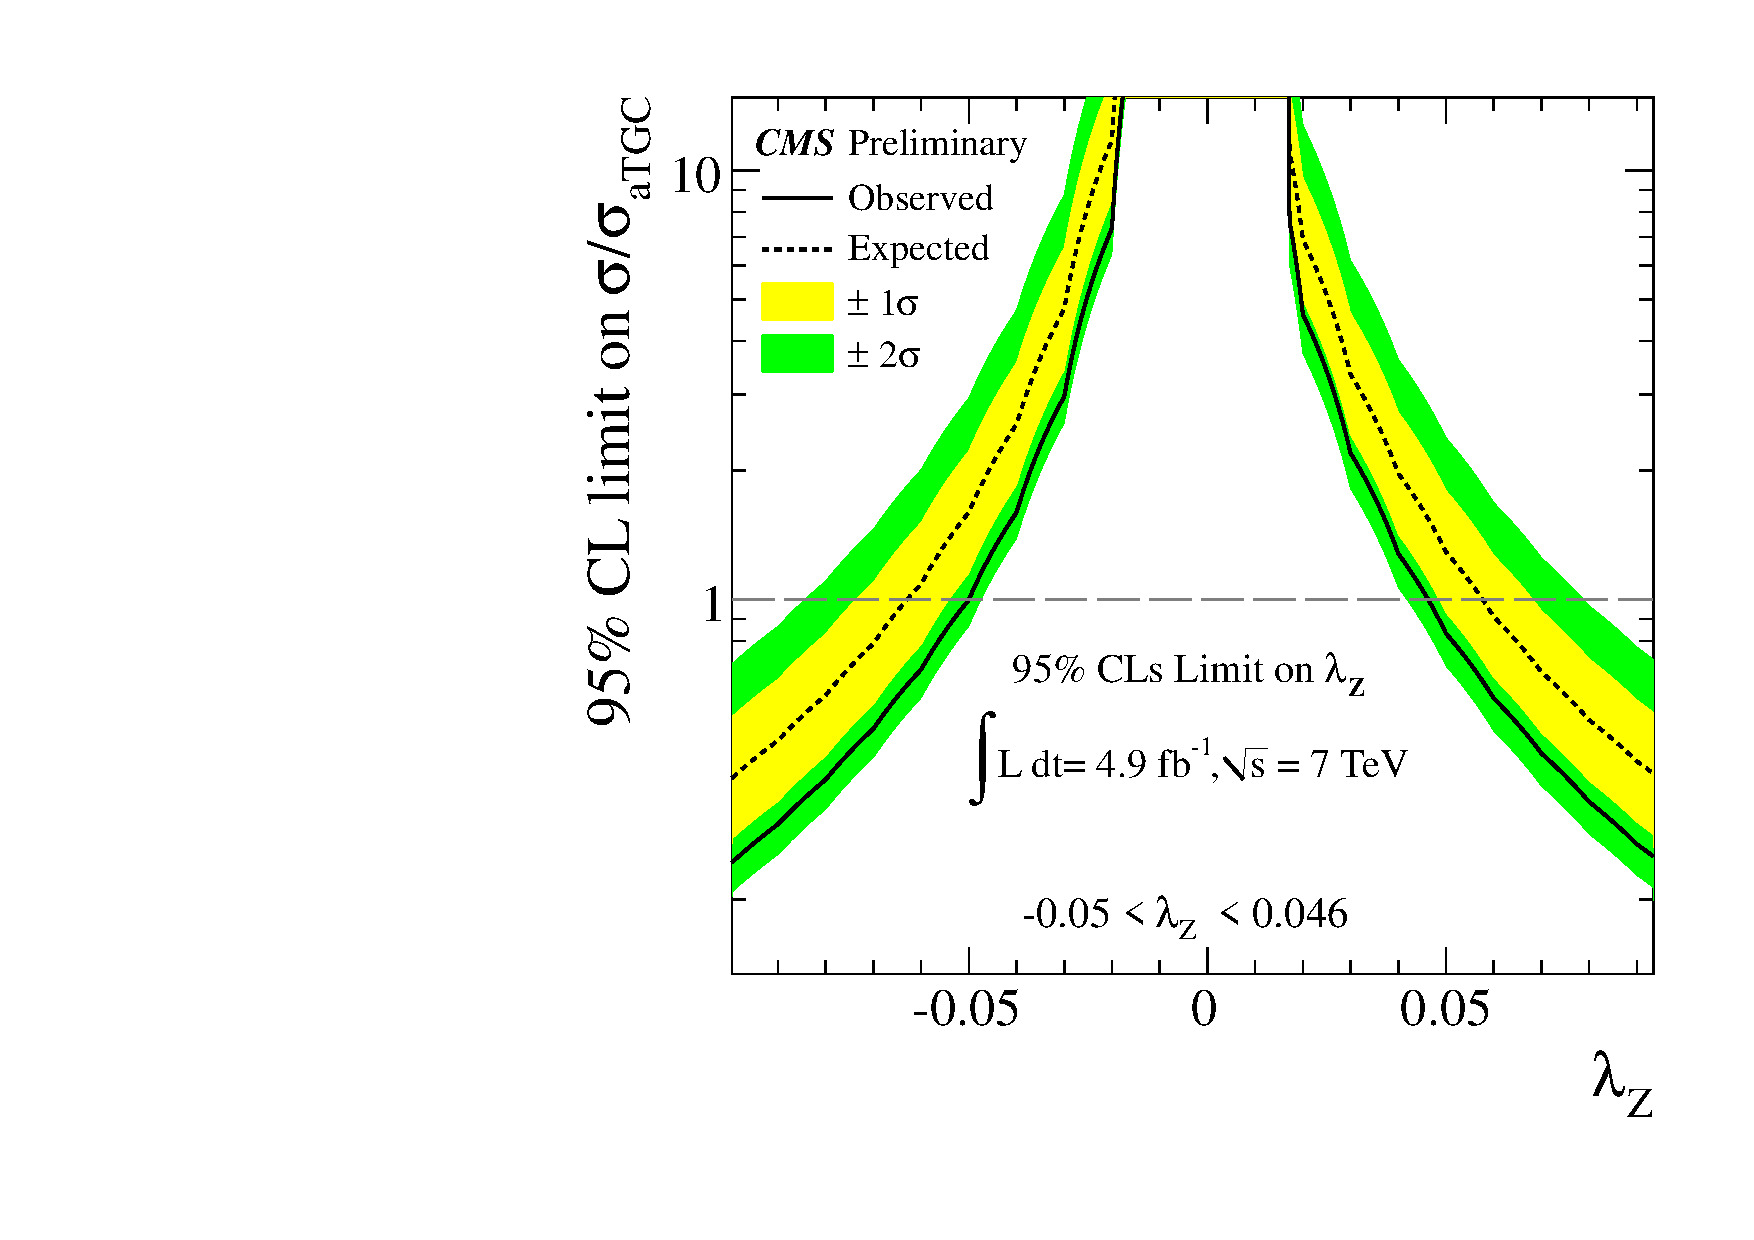
\includegraphics[width=.45\textwidth]{figures/lz_cls.pdf}
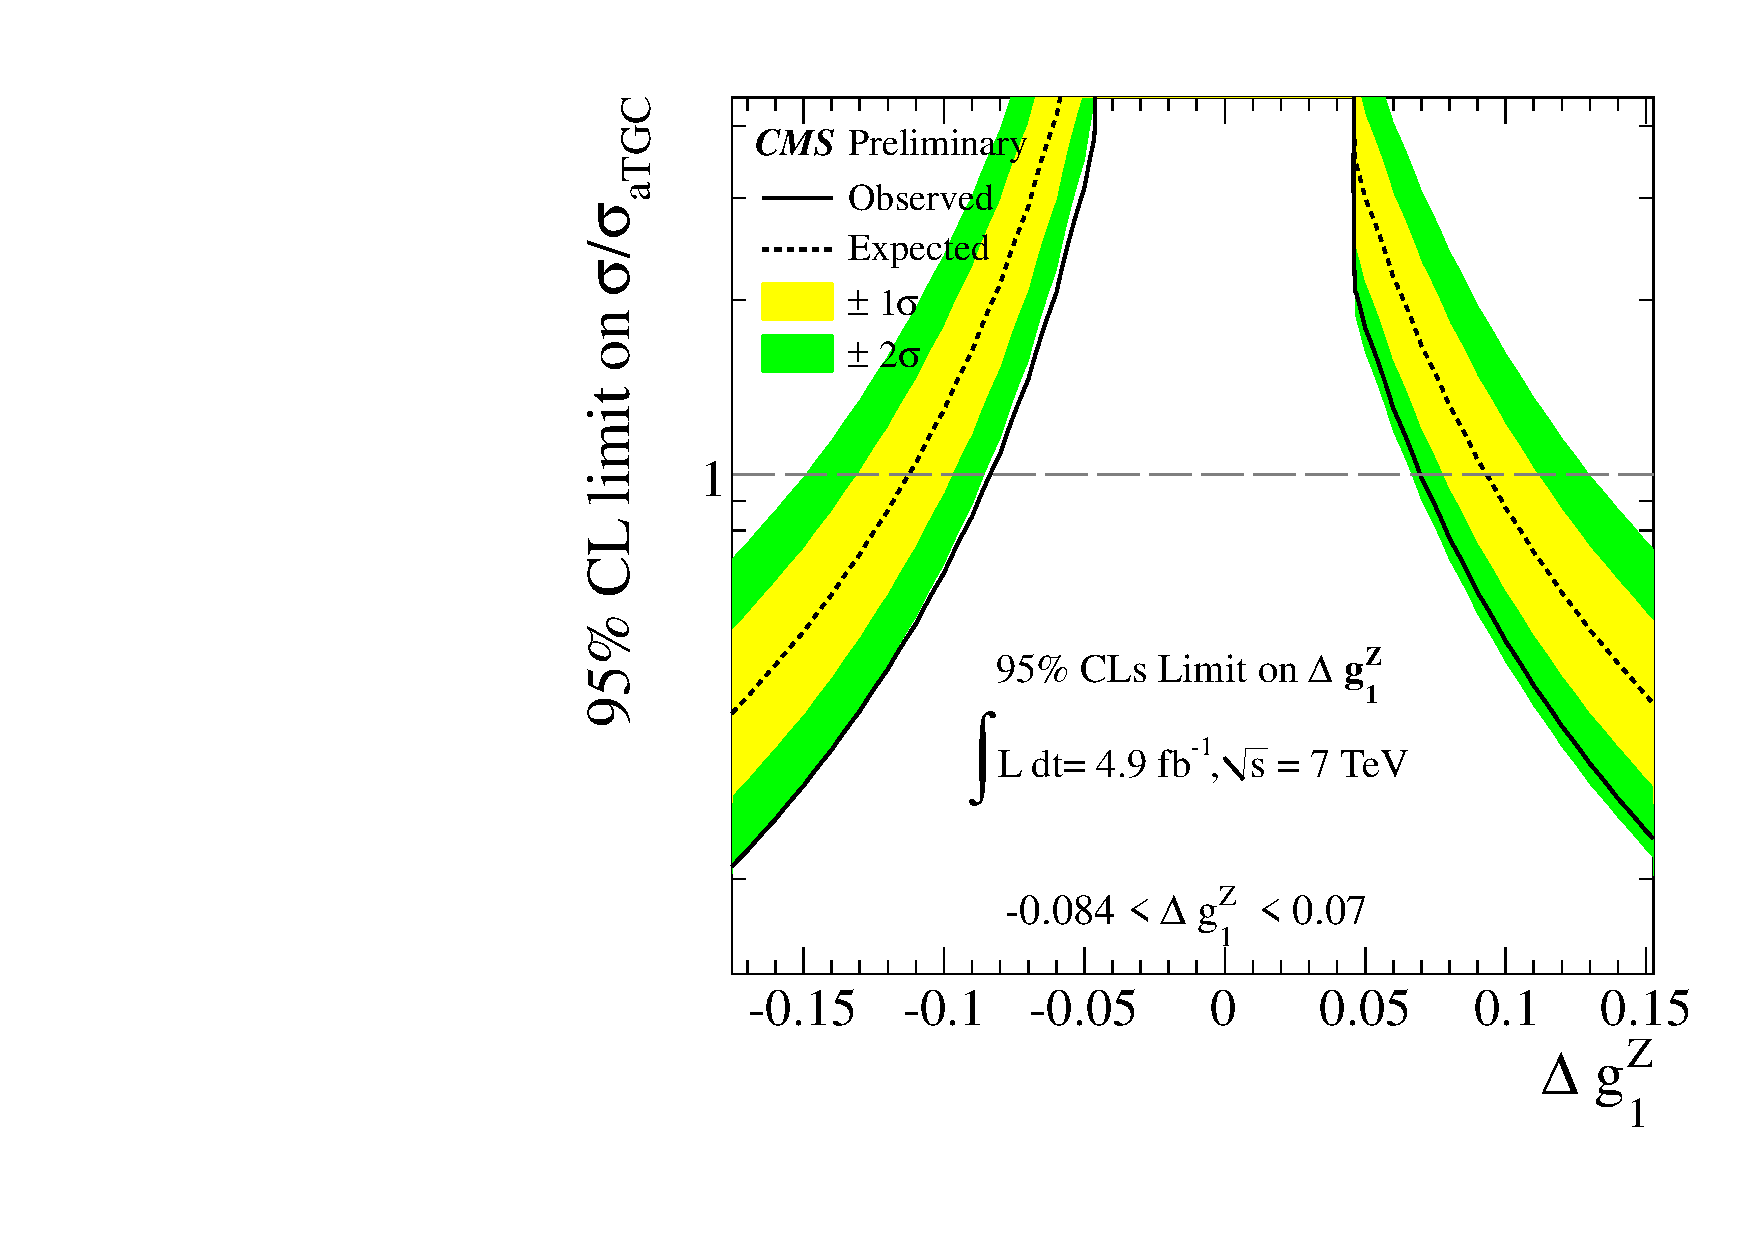
\includegraphics[width=.45\textwidth]{figures/dgz_cls.pdf}
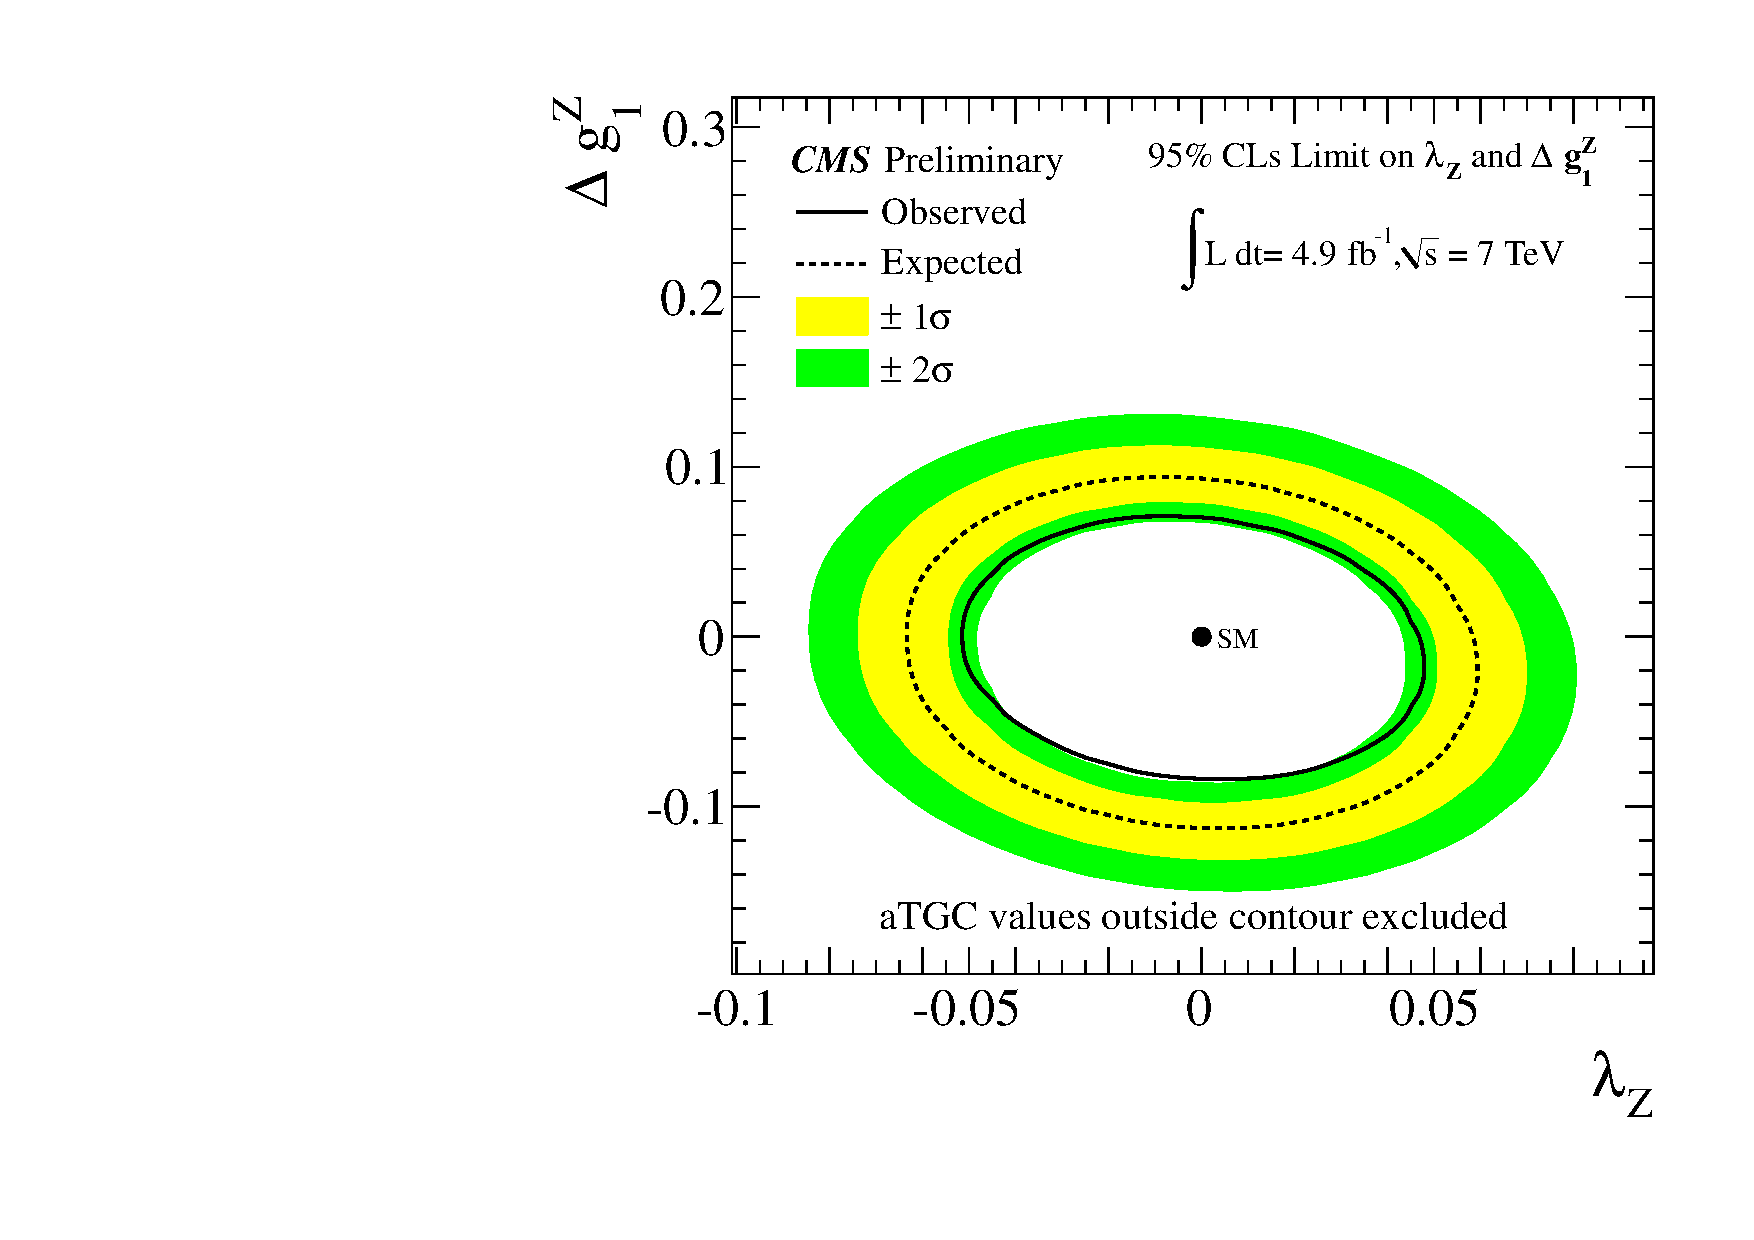
\includegraphics[width=.45\textwidth]{figures/lz_dgz_cls.pdf}
\caption{One and two dimensional $CL_{s}$ upper limits.}
\label{fig:cls}
\end{figure}

\end{document}
